\documentclass[a4paper, 12pt]{report}

% Margins: left 40mm, right 25mm, up and down 25mm
% Dimensions: 210mm x 297mm
% (warning, Latex default from left: 1in~25mm)

\usepackage{fullpage}
\addtolength{\hoffset}{0cm} % extends height of page
\addtolength{\textwidth}{0.5cm} % extends lenght of written text

% Everything about page geometry:
%https://www.sharelatex.com/learn/Page_size_and_margins

%% PRINTED VERSION
% uncomment this below to render text only on pages on the right side - for printed version
%\let\openright=\clearpage

%% ENCODINGS
\usepackage[utf8]{inputenc}
%\usepackage[IL2]{fontenc}
\usepackage[english]{babel}


%% PACKAGES
\usepackage{amsfonts}
\usepackage{amsmath}
\usepackage{amssymb}
\usepackage[font={footnotesize}]{caption}
\usepackage{csquotes}
\usepackage{enumerate}
\usepackage{epigraph}
\usepackage{graphicx}
\usepackage{setspace} % setup various spaces
\usepackage{titlesec}
\usepackage[titles]{tocloft}
\usepackage[labelfont={sf,bf}]{caption}
\usepackage{url}
\usepackage{wrapfig} % image wrapper
\usepackage{hyperref} % hyperlinks


%% MACROS
\newcommand{\unit}[1]{\,\mathrm{#1}} % nice units
\newcommand{\ind}[1]{\mathrm{#1}}
\newcommand{\He}{{}^4\mathrm{He}} % special Helium
\renewcommand{\Re}{\mathrm{Re}} % Reynolds number
\newcommand{\eps}{\varepsilon} % standard epsilon
\newcommand{\<}{\langle} % closed left
\renewcommand{\>}{\rangle} % closed right
\renewcommand{\vec}[1]{\mathbf{#1}} % nice bold vector
\renewcommand{\dot}{\!\cdot\!} % scalar product
\newcommand{\todo}[1]{ {\bf !!TODO!!}\qquad{#1} } % TODO marker

% optimal spacings
\setlength{\parskip}{9pt}
\setlength{\parindent}{0pt}
\setlength{\baselineskip}{1.2\baselineskip} % extend distance under equations

% The following part convinces Latex to not mess with the chapters...
\makeatletter
\def\@makechapterhead#1{
  {\parindent \z@ \raggedright \normalfont
   \Huge\bfseries \thechapter. #1
   \par\nobreak
   \vskip 20\p@
}}
\def\@makeschapterhead#1{
  {\parindent \z@ \raggedright \normalfont
   \Huge\bfseries #1
   \par\nobreak
   \vskip 20\p@
}}\newpage
\makeatother

% Defining a non-numbered chapter (but included in Summary)
\def\chapwithtoc#1{
\chapter*{#1}
\addcontentsline{toc}{chapter}{#1}
}

% Changing font of subsection
\titleformat{\subsection}
{\large\sffamily\bfseries}
{\thesubsection}{1.4em}{}


%%%%%%%%%%%%%%%%%%%%%%%%%%%%%%%%%%%%%%%%%%%%%%%%%%%%%%%%%%%%%%%%%%%%%%%%%%%%%%
%% FRONT PAGES
%%%%%%%%%%%%%%%%%%%%%%%%%%%%%%%%%%%%%%%%%%%%%%%%%%%%%%%%%%%%%%%%%%%%%%%%%%%%%%


\begin{document}
\pagestyle{empty}

% Cover page
\begin{center}
	\Large\sf
	Comenius University
	
	Faculty of Mathematics, Physics and Informatics
	\bigskip
	
	{
		\Huge \bfseries \sffamily DIPLOMA THESIS
	}
	
	\vfill
	
	
\includegraphics[width=0.5\textwidth]{graphics/fmfi_logo.jpg} 
	
	\vfill
	
	{
		\Huge\sf Jakub Bahyl
	}
	
	\vfill
	
	{
		\Huge \bfseries \sffamily
		\mbox{Quantum Turbulence}
		\mbox{Measurements in Superfluid Helium}
		\mbox{and Numerical Simulations}
	}
	
	\vfill

	\Large\sf
	Bratislava, 2018

\end{center}

\newpage

% Front page
\begin{center}
	\large\sf
	Comenius University

	Faculty of Mathematics, Physics and Informatics
	
	\bigskip

	{
		\Large \bfseries \sffamily 
		DIPLOMA THESIS
	}
	
	\vspace*{10mm}

	
\includegraphics[width=0.5\textwidth]{graphics/fmfi_logo.jpg} 

	\vfill
	\vspace*{5mm}

	{
		\LARGE\sf 
		Jakub Bahyl
	}

	\vspace*{5mm}

	{
		\LARGE \bfseries \sffamily
		\mbox{Quantum Turbulence}
		\mbox{Measurements in Superfluid Helium}
		\mbox{and Numerical Simulations}
	}

	\vfill

	Department of Low Temperature Physics, Charles University in Prague

	\vfill

	\begin{tabular}{rl}

	Study programme: & Condensed Matter Physics \\
	\noalign{\vspace{1mm}}
	Study programme number: & mFTL \\
	\noalign{\vspace{1mm}}
	Supervisor of the thesis: & RNDr. David Schmoranzer, PhD. \\
	\noalign{\vspace{1mm}}
	Consultant of the thesis: & Mgr. Emil Varga \\

	\end{tabular}

	\vfill

	{
		\Large\sf Bratislava, 2018
	}

\end{center}

\newpage

% Formal ENG
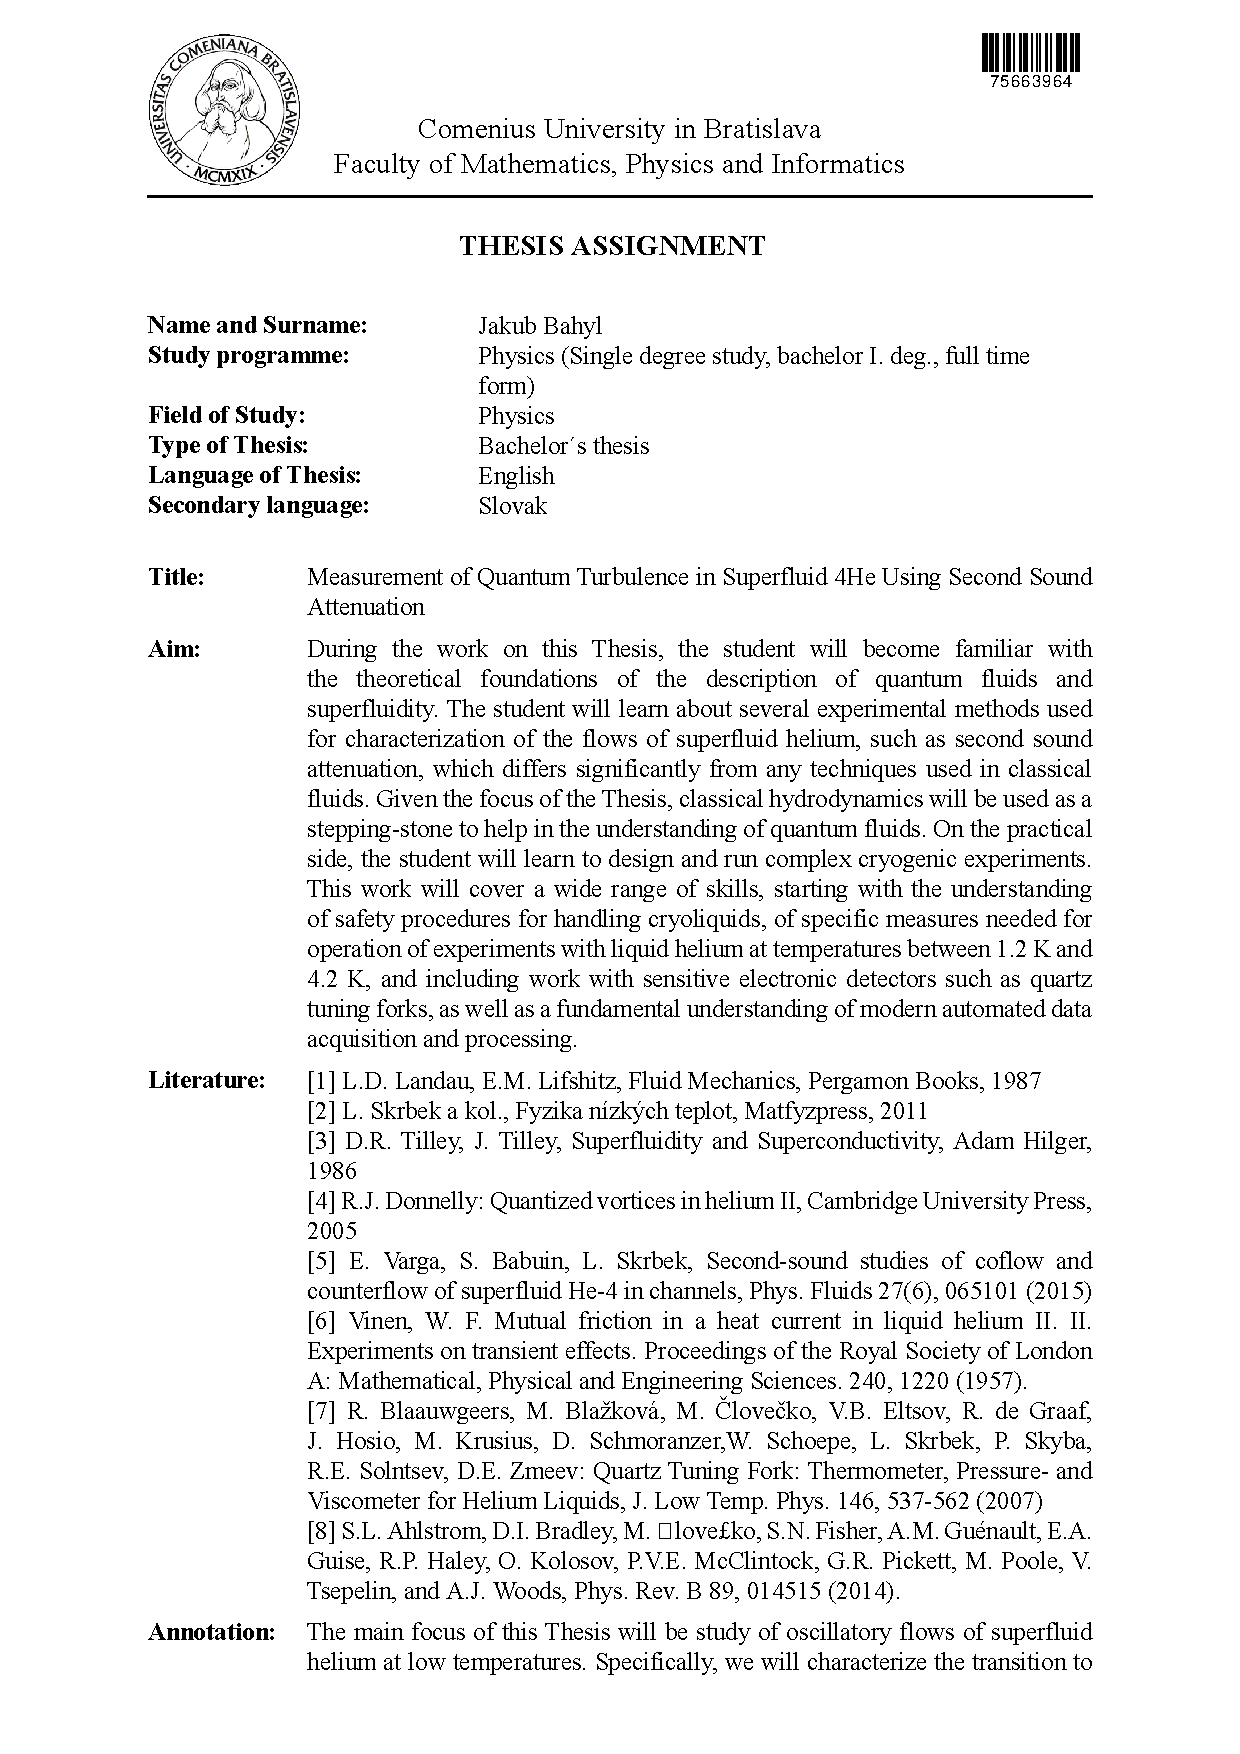
\includegraphics[width=0.9\textwidth]{docs/zadanie_Bahyl_EN.pdf}
\newpage

% Formal SVK
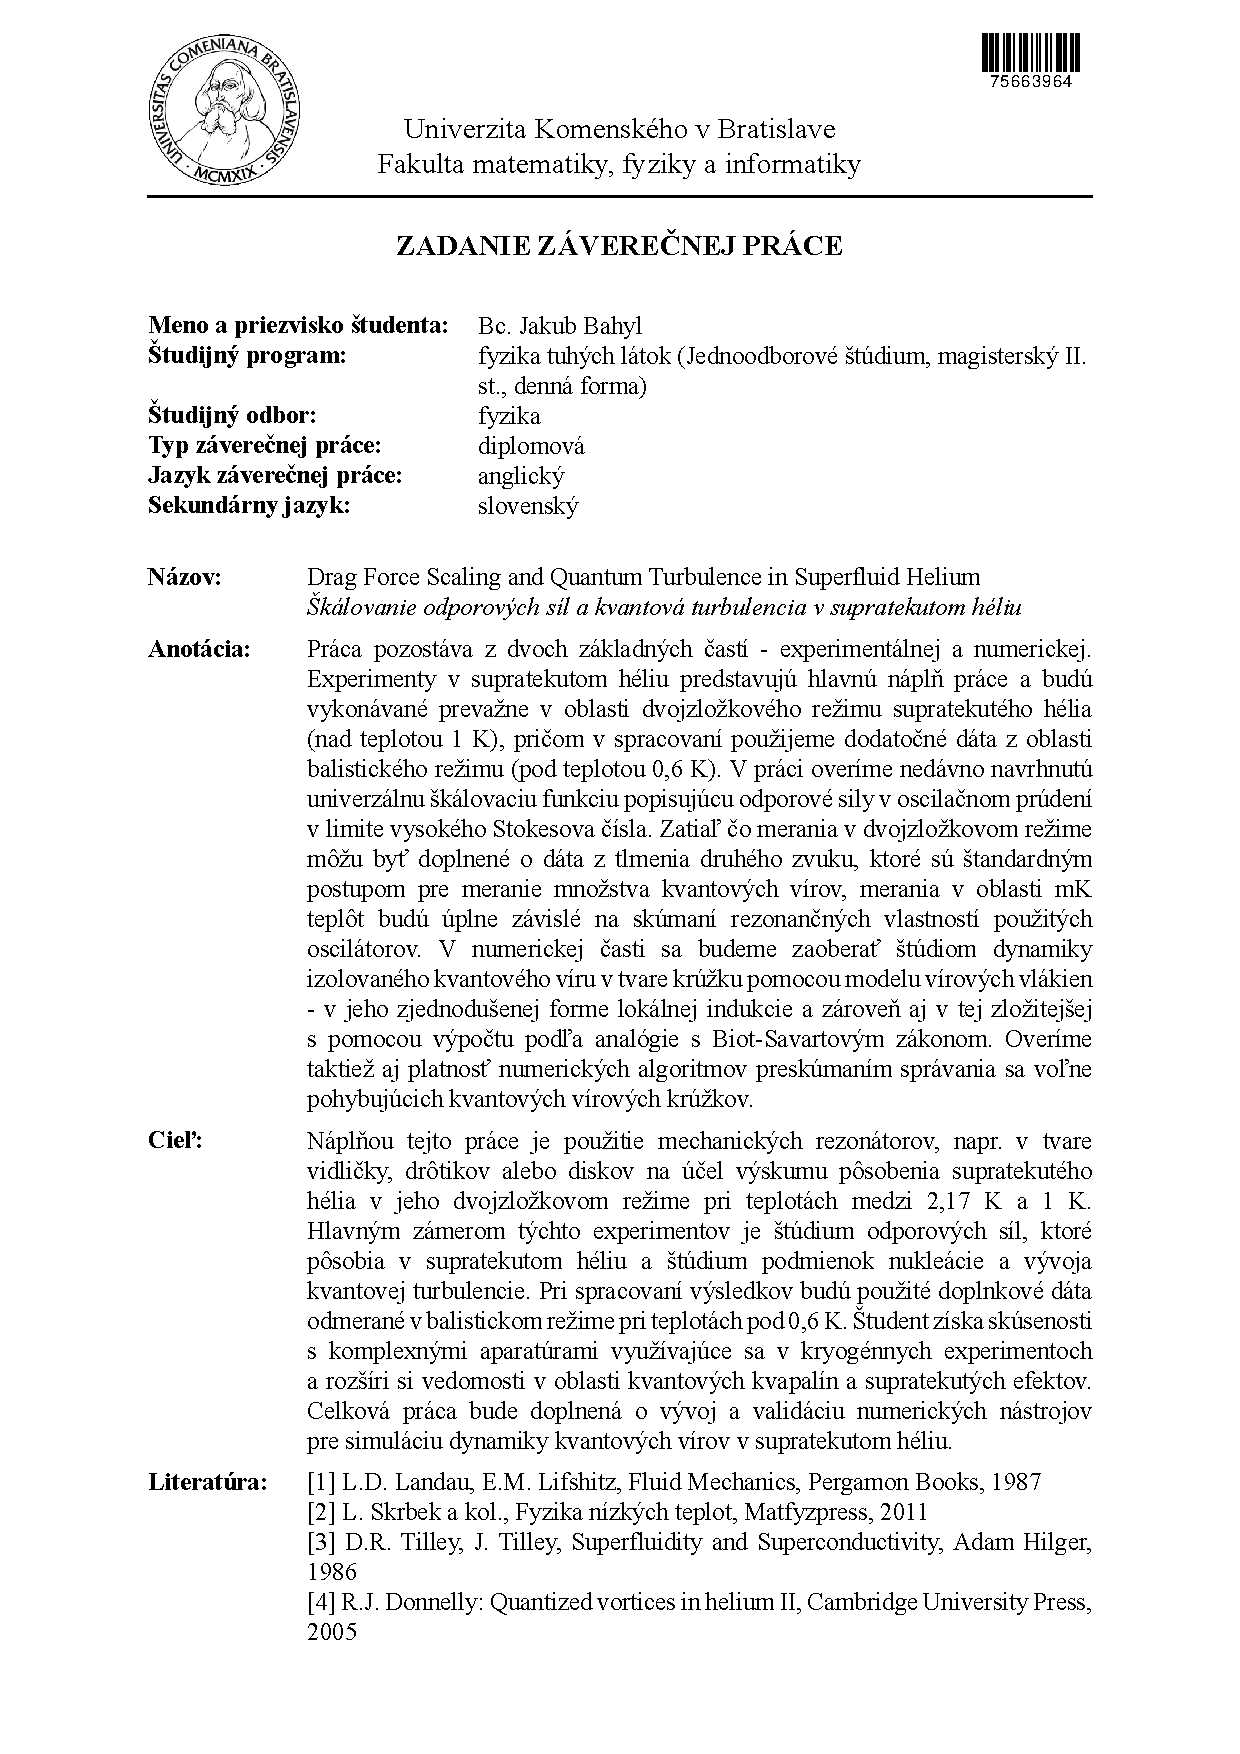
\includegraphics[width=0.9\textwidth]{docs/zadanie_Bahyl_SVK.pdf}
\newpage

% Acnkowledgements
\chapter*{Acknowledgment}
\pagenumbering{gobble}

BACHELOR:
My special thanks go to my supervisor, David Schmoranzer, who gave me a  lot of experiences, knowledge and much more of his time, without which I definitely could not write this Thesis. Together with consultant Martin Jackson, they guided me during the whole experiment and helped me to understand all the important aspects included in this work. Moreover, I am thankful to Ladislav Skrbek and Patrik Švančara for giving me such a great opportunity to find out how astounding the experimental physics can be and to work with Superfluidity group within Charles University in Prague.

In the end, I would like to hugely thank my friends and family for all their \textit{„Good luck"} and \textit{„Keep going"} motivational quotes and other sort of supports, which I deeply appreciated.

DIPLOMA:
Thanks.
\todo{}

\vglue 0pt plus 1fill

\noindent
I declare that I carried out this master thesis independently, and only with the cited
sources, literature and other professional sources.


\vspace{10mm}

\hbox{
	\hbox to 0.5\hsize{%
		In \parbox[b]{2.5cm}{\dotfill}
		date \parbox[b]{2.5cm}{\dotfill}
	\hss}
	\hbox to 0.5\hsize{%
		Signature of the author:
		\hss}
	}

\newpage

% Summary
\vbox to \vsize{
\setlength\parskip{5mm}

{\bfseries \sffamily Názov práce}\\
Kvantová turbulencia v supratekutom héliu v teplotnej limite absolútnej nuly

{\bfseries \sffamily Autor}\\
Jakub Bahyl

{\bfseries \sffamily Školiteľ bakalárskej práce}\\
RNDr. David Schmoranzer, Ph.D.

{\bfseries \sffamily Abstrakt}\\
V tejto práci prezentujeme meranie kvantovej turbulencie generovanej oscilujúcim $ 6.5\unit{kHz} $ kremenným oscilátorom, ponoreným v supratekutom $ \He $ pri viacerých teplotách pod kritickou $ T_{\lambda} = 2.17\unit{K} $. Pozorovaná nelineárna odporová sila pôsobiaca na oscilátor je kvalitatívne spôsobená prítomnosťou klasickej turbulencie a kvantovaných vírov. Odporové sily a množstvo vytvorených kvantovaných vírov (hustota vírov čiar $ L $) sú nepriamo určené z útlmu druhého zvuku a mechanicko-elektrických vlastností oscilátora.
Výsledky, ktoré prezentujeme, kvantitatívne charakterizujú tvorbu klasickej aj kvantovej turbulencie. Ako prví ukazujeme, že obidve turbulencie vedia vzniknúť samostatne a nezávisle. Tento fakt je prezentovaný, v prvom priblížení, pomocou \textit{prúdového fázového diagramu}, v ktorom pre danú teplotu vieme predpokladať, kedy a ktorá turbulencia vzniká.

{\bfseries \sffamily Kľúčové slová}\\
supratekutosť $ \He $ $\bullet$ kvantový vír a turbulencia

\noindent\rule{16cm}{0.5pt}

{\bfseries \sffamily Title}\\
Quantum turbulence in superfluid helium down to the zero temperature limit

{\bfseries \sffamily Author}\\
Jakub Bahyl

{\bfseries \sffamily Supervisor}\\
RNDr. David Schmoranzer, Ph.D.

{\bfseries \sffamily Abstract}\\
In this Thesis, mechanical resonators such as \textit{tuning forks, wires are discs} are used to probe superfluid helium in the two-fluid regime at temperatures between temperatures $1.0\unit{K} < T < 2.17\unit{K}$. The principal aim of the experimental part is to study the drag forces arising from the superfluid and the nucleation and development of quantum turbulence. The obtained data, also with those from the ballistic regime $ T < 0.6\unit{K}$, are used to test a proposed \textit{Universal scaling relation} describing the drag forces in high-Stokes-number oscillatory flow.\\
The experimental work is complemented by developing and validating the tools necessary for numerical simulations of quantized vortex dynamics in superfluid helium. In this part, dynamics of a single quantized vortex ring are studied using the \textit{Vortex filament model}.


{\bfseries \sffamily Keywords}\\
superfluidity of $ \He $  $\bullet$ quantum vortex and turbulence

\vss}

\newpage
\newpage

%%%%%%%%%%%%%%%%%%%%%%%%%%%%%%%%%%%%%%%%%%%%%%%%%%%%%%%%%%%%%%%%%%%%%%%%%%%%%%
%% THESIS
%%%%%%%%%%%%%%%%%%%%%%%%%%%%%%%%%%%%%%%%%%%%%%%%%%%%%%%%%%%%%%%%%%%%%%%%%%%%%%

\pagenumbering{arabic}
\pagestyle{plain}
\setcounter{page}{1}

% Content
\tableofcontents

% Chapters
%\chapter*{Introduction}
\addcontentsline{toc}{chapter}{Introduction}

	To this day, turbulent motion of fluids remains the last unresolved problem of classical physics. They present many practical challenges across different areas of industry (f.e. weather prediction). Quantum turbulence, in contrast, may occur only in superfluids and was first observed in superfluid state of $\He$. Compared to classical turbulence, it can be regarded as a simpler system from the theoretical and numerical point of view. Also, it shares many of the general properties of turbulence in classical viscous fluids.

	In very low temperatures, the liquid state of $\He$ exists in two phases:
	\begin{itemize}
		\item \underline{Helium-I}: a high temperature phase ($2.17\unit{K}<T<4.2\unit{K}$)
		\item \underline{Helium-II}: a low temperature phase ($T<2.17\unit{K}$)
	\end{itemize}

	These two phases are connected with the \textit{lambda transition}, which occurs at the critical temperature $T_{\lambda} = 2.17 \unit{K}$ at saturated vapour pressure (\textbf{Figure \ref{phase_diag}}). Helium-I is a classical fluid described by ordinary Navier-Stokes (N-S) equations, whereas Helium-II is a superfluid and behaves partly like a Bose-Einstein condensate.

	\begin{figure}[h]
		\centering
		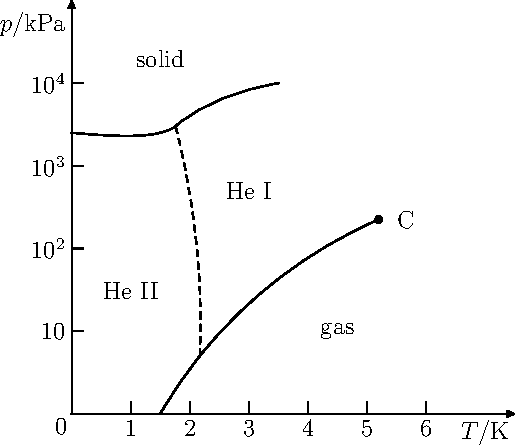
\includegraphics[width=0.6\textwidth]{graphics/theory/phase_diag}
		\caption{Pressure-Temperature diagram of $\He$. Fixing pressure on an atmospheric value, a gas-liquid transition is present at $4.2\unit{K}$ (He-I) and a superfluid transition at $2.17\unit{K}$.}
		\label{phase_diag}
	\end{figure}

	A simple, phenomenological model of the Helium-II motion was proposed by Tisza \cite{tisza} and Landau \cite{landau} - the \textit{two-fluid model}. According to two-fluid model, it behaves as if composed of two inter-penetrating liquids - the normal and superfluid components - with corresponding velocity fields and temperature-dependent densities:

	\begin{itemize}
		\item \underline{normal component}: density $\rho_n (T)$, velocity field $\vec{v}_n (\vec{r}, t)$, motion described by an ordinary viscous Navier-Stokes equation, carrying entropy and represented as a collection of thermal excitations such as \textit{phonons} and \textit{rotons}
		\item \underline{superfluid component}: density $\rho_s (T)$, velocity field $\vec{v}_s(\vec{r}, t)$, motion described by a modified Euler equation (without viscosity) with quantum terms, no entropy and represented by a macroscopic wave function
	\end{itemize}

	The total density of Helium-II sums up to $\rho = \rho_n(T) + \rho_s(T) \approx \text{const}$ and the relative proportion of normal/superfluid component is determined mainly by the temperature (\textbf{Figure \ref{densities}}). Near $T \rightarrow 0$ Helium-II becomes entirely superfluid $\rho_s/\rho \rightarrow 1$. The temperature dependence of this ratio is highly nonlinear. For example, the ratio $\rho_n/\rho$ drops from $100\%$ at $2.17\unit{K}$ to $50\%$ at $1.95\unit{K}$, to $<5\%$ at $1.3\unit{K}$, and is effectively negligible under $1\unit{K}$.

	\begin{figure}[h]
		\centering
		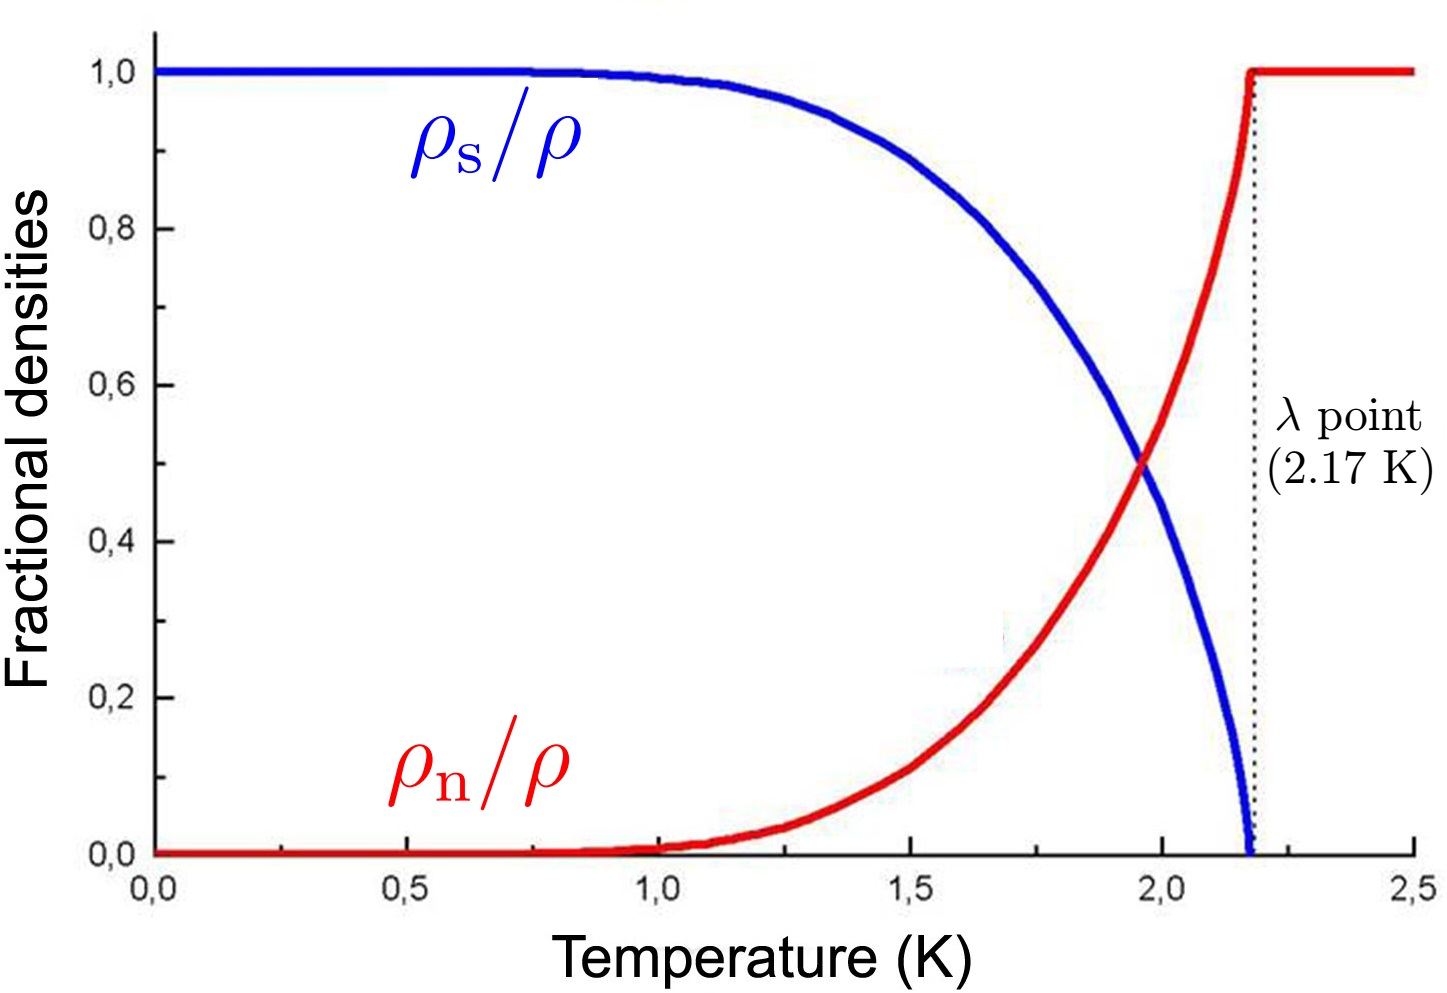
\includegraphics[width=0.6\textwidth]{graphics/theory/densities}
		\caption{Temperature dependence of fractional densities of the normal (red) and superfluid (blue) components. Source: \cite{svoc2016}}
		\label{densities}
	\end{figure}

	It arises from the quantum nature of superfluid, that the superfluid component should not perform any rotation. However, when this component moves faster than a critical velocity, the circulation is \textit{quantized} and so-called \textit{quantized vortices} are created, which makes the hydrodynamics of Helium-II particularly interesting. The vortex nucleation process is still a subject of many current investigations. Superfluid vortex lines were observed spatially organized, but also completely disorganized as simulated in \textbf{Figure \ref{sim_cube}}. Quantum turbulence therefore takes the form of a tangle of quantized vortices in the superfluid component which typically coexist with classical turbulent flow of the normal component.

	In the presence of quantized vortices, the independent normal and superfluid velocity fields become coupled by the \textit{mutual friction} force which arises due to quasiparticles scattering off the cores of vortices.

	\begin{figure}[h]
		\centering
		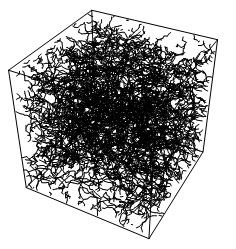
\includegraphics[width=0.4\textwidth]{graphics/theory/QT-tangle}
		\caption{Cube of numerically simulated tangle of randomly distributed quantised vortices. Source: \cite{svoc2016}}
		\label{sim_cube}
	\end{figure}

	Also we note that for a typical experiment, below $\sim 0.7\unit{K}$, a transition to ballistic regime occurs in the normal component, as the mean free path of phonons exceeds the characteristic dimensions of the experimental setup. This situation is similar to the one of dilute classical gases.

	Quantum turbulence can be experimentally achieved in many traditional ways - driving a mass flow, spinning discs, oscillating grids and forks, ultrasound and jets.\\
	To characterize the turbulence one may use a superfluid Reynolds number for a steady flows, or a newly introduced \cite{universal_scaling} Donnelly number for high-frequency oscillatory flows.
	We find that for quantum turbulence originated in high-frequency regime above temperature $T > 1\unit{K}$, the measured drag forces are described in terms of a single dimensionless parameter and exhibit an universal scaling behaviour. We identify and compare the critical conditions related to the production of both quantized vorticity and instabilities occuring in normal component.

	Besides experimental approaches on quantum fluids, one of the useful tools for understanding the geometry and flow of quantum turbulence, is the \textit{vortex filament model}, pioneered by Schwarz \cite{schwarz}. With the rapid development of available computational power, large simulations have become the methods of choice for calculating the motion of fluids. In superfluids like Helium-II, due to the quantization of circulation, vorticity can only exist within vortex filaments with a certain core size, which makes the model highly applicable.

	We propose an efficient numerical method to compute the time evolution of vortex filaments in superfluid Helium-II. We studied the performance and stability and well replicated the physical processes such as the annihilation of quantized vortex rings \cite{vortex_ring} while travelling across superfluid.\\
	We also present the \texttt{PyVort} code, a new platform in Python 3 to simulate quantized rings phenomena. More on the implementation part can be found in \textbf{Simulation} and \textbf{Appendix}.

%%%%%%%%%%%%%%%%%%%%%%%%%%%%%%%%%%%%%%%%%%%%%%%%%%%%%%%%%%%%%%%%%%%%%%%%%%%%%%

	\section*{Motivations and Goals}

	Here we briefly collect all motivations and goals that led us to our investigations.

	\subsection*{Experimental approach}

	\begin{itemize}
		\item ivestigate transition from laminar and potential flow of normal and superlfuid components, respectively, to classical or quantum turbulence at various temperatures above $>1\unit{K}$ in high-frequency regime.
		\item construct an experiment using flow generators such as vibrating wire, tuning fork and oscillating disc and observe the drag phenomena
		\item apply universal scaling theory and prove the concept on collected experimental data
	\end{itemize}

	\subsection*{Simulation}
	\begin{itemize}
		\item build modular and reusable codebase in Python 3 that simulates the dynamics of quantized vortices using the \textit{Vortex Filament} model
		\item implement stable time-step methods and a reliable re-segmentation process that allows keeping a good resolution of quantized vortices in different situations
		\item simulate a real-time quantum vortex ring motion and compare its properties and evolution in time with the theoretical approaches, thus validating the new codebase
	\end{itemize}

\newpage

%%%%%%%%%%%%%%%%%%%%%%%%%%%%%%%%%%%%%%%%%%%%%%%%%%%%%%%%%%%%%%%%%%%%%%%%%%%%%%
%%%%%%%%%%%%%%%%%%%%%%%%%%%%%%%%%%%%%%%%%%%%%%%%%%%%%%%%%%%%%%%%%%%%%%%%%%%%%%
%%%%%%%%%%%%%%%%%%%%%%%%%%%%%%%%%%%%%%%%%%%%%%%%%%%%%%%%%%%%%%%%%%%%%%%%%%%%%%

\chapter{Theoretical Background}

The theoretical part of this Thesis is composed of two chapters:

\begin{itemize}
	\item[1.] \underline{Micro/Meso-scopic view} - provides a theoretical cover of Gross-Pitaevskii model, creation and numerical modelling of the quantized vortex and its dynamics.

	\item[3.] \underline{Macroscopic view} - provides a hydrodynamics description of two-fluid model, oscillatory motion in He-II, creation of quantum turbulence, dynamical and universal scaling principles

\end{itemize}

The aim of the theoretical part is to introduce the basic properties of quantized vortex lines in Helium-II and summarize the state of art of current knowledge on superfluid turbulence. We also discuss the theoretical methods used to study quantized vorticity, quantum turbulence and the results obtained using such methods.

%%%%%%%%%%%%%%%%%%%%%%%%%%%%%%%%%%%%%%%%%%%%%%%%%%%%%%%%%%%%%%%%%%%%%%%%%%%%%%
%%%%%%%%%%%%%%%%%%%%%%%%%%%%%%%%%%%%%%%%%%%%%%%%%%%%%%%%%%%%%%%%%%%%%%%%%%%%%%

\newpage

{\Huge \bfseries Micro/Meso-scopic view}
\addcontentsline{toc}{chapter}{Micro/Meso-scopic model}
\vspace{0.3cm}

One of the most useful ways of describing superfluid $\He$ at $T=0\unit{K}$ starts with nonlinear Schrodinger equation (NLSE) for the one-particle wave function $\psi$. Since the superfluid $\He$ is a strongly correlated system dominated by collective effects, this imperfect Bose-Einstein condensate (BEC) is approximately described by Gross-Pitaevskii equation (\ref{gross-pit}). Although, it must be noted that the real Helium-II is a dense fluid, not a weakly interacting Bose gas described by NLSE.

%%%%%%%%%%%%%%%%%%%%%%%%%%%%%%%%%%%%%%%%%%%%%%%%%%%%%%%%%%%%%%%%%%%%%%%%%%%%%%

\section{Gross-Pitaevskii model}

In terms of single-particle wavefunction $\psi(\vec{r},t)$ we write the Gross-Pitaevskii model:

\begin{equation}
i \hbar \frac{\partial \psi}{\partial t} = - \frac{\hbar^2}{2m} \nabla^2 \psi
+ \psi \int \vert \psi(\vec{r}^{\prime},t) \vert^2 V(\vert \vec{r} - \vec{r}^{\prime} \vert)
\text{d}\vec{r}^{\prime}\,,
\label{gross-pit}
\end{equation}

where $V(\vert \vec{r} - \vec{r}^{\prime} \vert)$ is the potential of two-body interaction between bosons. The normalization is set as $\int \vert \psi \vert^2 \text{d}\vec{r} = N$, where $N$ is number of bosons. By replacing potential with repulsive $\delta$-function of strength $V_0$ one obtains:

\begin{equation}
i \hbar \frac{\partial \Psi}{\partial t} = - \frac{\hbar^2}{2m} \nabla^2 \Psi - m\eps \Psi + V_0 \vert \Psi \vert^2 \Psi\,,
\label{GP}
\end{equation}

where $\eps$ is the energy per unit mass and $\Psi = A e^{i\Phi}$ is a macroscopic wave function of condensate. In this way one can define the condensate's density $\rho_{BEC} = m\Psi\Psi^* =  mA^2$ and velocity $\vec{v}_{BEC} = (\hbar / m)\nabla \Psi$. Note that equation (\ref{GP}) is equivalent to a continuity equation and an modified Euler equation (by the so called quantum pressure term).

Hereafter we identify $\rho_{BEC}$ with $\He$ superfluid component's $\rho_s$ at absolute zero and $\vec{v}_{BEC}$ with $\vec{v}_s$. It must be noted that this identification is convenient from the point of view of having a simple hydrodynamics model but is not entirely correct. The reason is
that Helium-II is a dense fluid, not the weakly interacting Bose gas described
by the NLSE (\ref{gross-pit}), so the condensate is not the same as the superfluid component.

\newpage

Even though the superfluid is irrotational: $\omega = \nabla \times \vec{v}_s = \vec{0}$, the NLSE has a vortex-like solution: $\vec{v}_s = \varkappa / 2\pi r\, \vec{e_{\theta}}$, where $\theta$ is the azimuthal angle and $\varkappa=9.97 \times 10^{-4} \unit{cm^2 \dotprod s^{-1}}$ is the \textit{quantum of circulation}, obtained from:

\begin{equation}
\varkappa = \oint_{\mathcal{C}} \vec{v}_{BEC} \cdot \unit{d}\vec{\boldsymbol{\ell}} = \frac{h}{m}\,,
\label{varkappa}
\end{equation}

where $\mathcal{C}$ is a closed loop surrounding the vortex core - a topological defect (\textbf{Figure {\ref{singularity}}}) within macroscopic wavefunction $\Psi$

\begin{figure}[h]
	\centering
	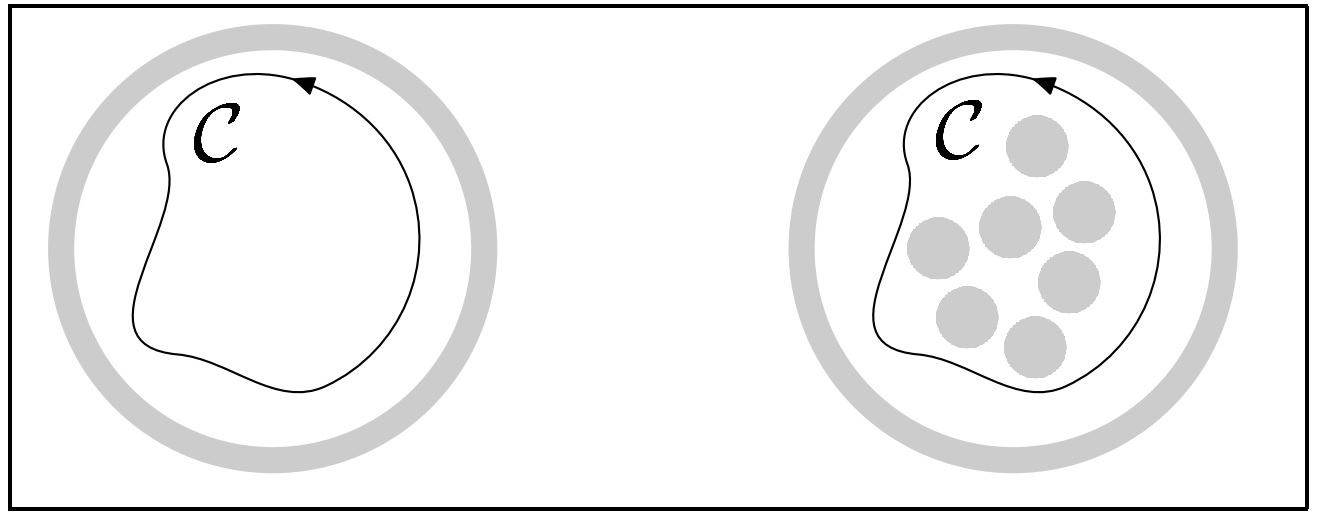
\includegraphics[width=0.6\textwidth]{graphics/theory/singularity}
	\caption{An illustration of topological singularities within a superfluid $\He$. Left: A singly-connected irrotational region with circulation along $\mathcal{C}$ loop equal to zero. Right: A multiply-connected region with depicted cores of quantized vortices with a finite circulation along $\mathcal{C}$ loop.}
	\label{singularity}
\end{figure}

%%%%%%%%%%%%%%%%%%%%%%%%%%%%%%%%%%%%%%%%%%%%%%%%%%%%%%%%%%%%%%%%%%%%%%%%%%%%%%

\section{Quantized vortex}

As Feynman showed \cite{feynman}, superfluid vortex lines appear when Helium-II moves faster than a certain critical velocity. The simplest way to create quantum vortices is to rotate cylinder with superfluid Helium-II with high enough angular velocity $\Omega$. Created vortex lines form an ordered array of density $L=2\Omega / \varkappa$, all aligned along the axis of rotation (\textbf{Figure \ref{rotating-helium}}). \textit{Vortex line density} $L$ can be also interpreted as a total vortex length in an unit volume.

\begin{figure}[h]
	\centering
	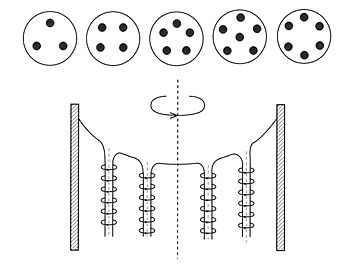
\includegraphics[width=0.4\textwidth]{graphics/theory/rotating-helium}
	\caption{Array of quantized vortices in a rotating container}
	\label{rotating-helium}
\end{figure}

The key properties of Onsager-Feynman vortex \cite{onsager} are the quantized circulation $\varkappa$, superfluid rotational velocity field $\vec{v}_s = \varkappa / 2\pi r\, \vec{e_{\theta}}$ and the \textit{vortex core parameter} $a_0$. The core size $a_0$ can be estimated by substituting $\vec{v}_s$ back into (\ref{GP}) and solving differential equation for $\rho_s$. One finds that $\rho_s$ tends to the value $m^2 \eps / V_0$ for $r \rightarrow \infty$ and to zero density for $r \rightarrow 0$.
The characteristic distance over which $\Psi$ collapses (superfluid density $\rho_s$ drops from bulk value to zero) is $a_0 \approx 10^{-10} \unit{m} = 1 \unit{\AA}$. From this, there is a conclusion that the vortex is hollow at its core and therefore, a topological defect occurs.

Taking $a_0$ as core radius, the energy considerations showed that a single vortex containing $N$ circulation quanta owns more energy than $N$ singly-quantized vortices. Hence it is generally assumed that only ground-state vortices are commonly observed.

Clearly, vortex lines don't have to be aligned in general. In most cases , the superfluid flow is strongly chaotic, better known as \textit{quantum turbulence}. This topic is covered in more detail later in this work.

%%%%%%%%%%%%%%%%%%%%%%%%%%%%%%%%%%%%%%%%%%%%%%%%%%%%%%%%%%%%%%%%%%%%%%%%%%%%%%

\section{Vortex filament model}

The vortex line can be represented as a curve via position vector $\vec{s} = \vec{s}(\xi, t)$ in three-dimensional space. Here, $\xi$ is arclength along the vortex line. Next we label $\vec{s}^{\prime}$ as $\text{d}\vec{s} / \text{d} \xi$ and $\vec{s}^{\prime\prime}$ as $\text{d}\vec{s}^{\prime} / \text{d} \xi$.
Within our context, $\vec{s}^{\prime}$ is a tangent vector and $\vert \vec{s}^{\prime\prime} \vert$ is a local curvature $R^{-1}$ at a given point.
The triad of vectors $\vec{s}^{\prime}$, $\vec{s}^{\prime\prime}$, $\vec{s}^{\prime} \times \vec{s}^{\prime\prime}$ are perpendicular to each other (\textbf{Figure \ref{filament}}) and point along the tangent, normal and binormal respectively:

\begin{figure}[h]
	\centering
	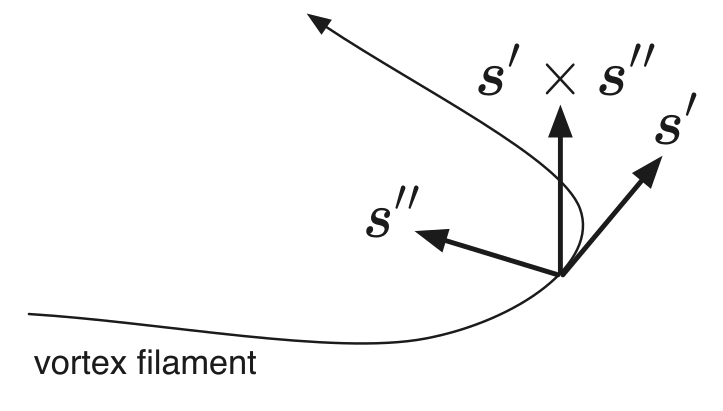
\includegraphics[width=0.7\textwidth]{graphics/theory/filament}
	\caption{Schematic of the vortex filament and the triad vectors $\vec{s}^{\prime}$, $\vec{s}^{\prime\prime}$, $\vec{s}^{\prime} \times \vec{s}^{\prime\prime}$. Source: \cite{tsubota}}
	\label{filament}
\end{figure}

We suppose that the superfluid component is incompressible $\nabla \dotprod \vec{v}_s = 0$. Moreover, superfluid vorticity $\omega_s$ is localized only at positions of vortex filament $\omega_s(\vec{r},t) = \nabla \times \vec{v}_s$. Combining these two properties gives the Poisson equation $\Delta \phi = \omega_s$ for the potential $\phi$.
Using Fourier transform one obtains \cite{barenghi} the Biot-Savart law for the superfluid velocity:

\begin{equation}
\vec{v}_s(\vec{r}) = \frac{\varkappa}{4\pi} \int_{\mathcal{L}} \frac{(\vec{r^{\prime}} - \vec{r}) \times \text{d}\vec{r^{\prime}}}{\vert \vec{r^{\prime}} - \vec{r} \vert^3}\,,
\label{biot_general}
\end{equation}

where the integral path $\mathcal{L}$ represents curves along all vortex filaments.

This law determines the superfluid velocity field $\vec{v}_s(\vec{r})$ via the arrangement of the vortex filaments. Now we define the \textit{self-induced} velocity $\vec{v}_{\text{ind}}$, describing the motion which a vortex line induces onto itself ($\vec{r} \rightarrow \vec{s}$ in (\ref{biot_general})) due to its own curvatures:

\begin{equation}
\vec{v}_{\text{ind}}(\vec{s}) = \frac{\varkappa}{4\pi} \int_{\mathcal{L}} \frac{(\vec{r^{\prime}} - \vec{s}) \times \text{d}\vec{r^{\prime}}}{\vert \vec{r^{\prime}} - \vec{s} \vert^3}
\label{biot_ind}
\end{equation}

However, this integral (\ref{biot_ind}) diverges as $\vec{r}^{\prime} \rightarrow \vec{s}$ because the core structure
of the quantized vortex was initially neglected. We avoid this divergence by splitting the integral into two parts - direct neighbourhood of the point $\vec{s}$ (local part) and the rest $\mathcal{L}^{\prime}$ (nonlocal part). The Taylor expansion of the local part leads \cite{schwarz} to a finite result:

\begin{align}
\vec{v}_{\text{ind}}(\vec{s})
= \vec{v}_{\text{ind,local}} + \vec{v}_{\text{ind,nonlocal}}
\approx& \beta \vec{s}^{\prime} \times \vec{s}^{\prime \prime} + \frac{\varkappa}{4\pi} \int_{\mathcal{L}^{\prime}} \frac{(\vec{r^{\prime}} - \vec{s}) \times \text{d}\vec{r^{\prime}}}{\vert \vec{r^{\prime}} - \vec{s} \vert^3}\,,
\label{lia+biot}
\\
\text{where}\, \beta =& \frac{\varkappa}{4\pi} \ln(R / a_0)\,,
\label{beta}
\end{align}

where $\mathcal{L}^{\prime}$ is the original vortex line without a close area of the studied vortex point and $R$ is a \textit{local curvature} and often is calculated as $1 / \vert \vec{s}^{\prime\prime} \vert$ \cite{schwarz}.

Since the local part of induced velocity (\ref{lia+biot}) is a dominant term (and also computationally faster), the nonlocal part can be neglected. Such approximation process is called as \textit{Local Induction Approximation} (LIA). LIA represents the contribution of local curvature to the induced velocity, whereas nonlocal Biot-Savart part represents the global filament curvature.

Since in the system there could be present also external flow sources of superfluid component (e.g. heat resistors causing \textit{counterflows}), we define the total superfluid velocity $\vec{v}_{s,tot}$, in a laboratory frame, as:

\begin{equation}
\vec{v}_{s,tot} = \vec{v}_{s,ext} + \vec{v}_{\text{ind}}
\end{equation}

\newpage

%%%%%%%%%%%%%%%%%%%%%%%%%%%%%%%%%%%%%%%%%%%%%%%%%%%%%%%%%%%%%%%%%%%%%%%%%%%%%%


\section{Vortex dynamics}

To determine the equation of motion of $\vec{s}(t)$ we recognize the forces acting upon the line - the magnus force $\vec{f}_M$ and (at non-zero temparature $T>0\unit{K}$ )the drag force $\vec{f}_D$ (both are per unit length).

The magnus force $\vec{f}_M$ always arises when a rotating body moves in a flow. This causes a pressure difference, which in our case of moving vortex line with circulation quantum $\varkappa$, exerts a force:

\begin{equation}
\vec{f}_M = \rho_s \varkappa \,\vec{s}^{\prime} \times (\vec{\dot{s}} - \vec{v}_{s,tot})\,,
\label{magnus}
\end{equation}

where $\vec{\dot{s}} = \text{d}\vec{s} / \text{d} t$ is the velocity of a particular point on a vortex line.

The drag force $\vec{f}_D$ arises from the \textit{mutual friction}, the interaction between the normal component and vortex lines (quantized superfluid component). According to the findings of Vinen and Hall \cite{vinen}, the normal fluid flowing with velocity $\vec{v}_n$ past a vortex core exerts a frictional force $\vec{f}_D$ on the vortex line, given by:

\begin{align}
\vec{f}_D = -& \alpha(T)\rho_s\varkappa\,\vec{s}^{\prime} \times [\vec{s}^{\prime} \times (\vec{v}_{ns} - \vec{v}_{\text{ind}})]
\label{alpha1}
\\
-& \alpha^{\prime}(T)\rho_s\varkappa\,\vec{s}^{\prime} \times (\vec{v}_{ns} - \vec{v}_{\text{ind}})
\,,
\label{alpha2}
\end{align}

where $\vec{v}_{ns} = \vec{v}_{n} - \vec{v}_{s,ext}$ is the difference between the average velocity of normal component and the applied superfluid velocity.

The temperature dependent dimensionless parameters $\alpha(T)$ and $\alpha^{\prime}(T)$ are often written in terms of measured \textit{mutual friction parameters} $B$ and $B^{\prime}$, which are known from experiments by Samuels and Donnelly \cite{donnelly}:

\begin{equation}
\alpha(T) = \frac{\rho_n B(T)}{2\rho}
\hspace{1cm}
\alpha^{\prime}(T) = \frac{\rho_n B^{\prime}(T)}{2\rho}
\end{equation}

The precise calculation of the mutual friction parameters $B(T), B^{\prime}(T)$ over the entire temperature range is still an open problem. Although, we already know that in the area of high temperatures, the friction arises mainly from the scattering processes of rotons.

\newpage

Since the mass of vortex core is usually neglected, the two forces $\vec{f}_M$ and $\vec{f}_D$ add up to zero: $\vec{f}_M + \vec{f}_D = \vec{0}$. Hence, solving for $\text{d}\vec{s} / \text{d} t$, we obtain \cite{schwarz} the Schwarz's equation:

\begin{equation}
\dot{s} = \vec{v}_{\text{s, ext}} + \vec{v}_{\text{ind}}
+ \alpha\vec{s}^{\prime} \times (\vec{v}_{ns} - \vec{v}_{\text{ind}})
- \alpha^{\prime}\vec{s}^{\prime} \times [\vec{s}^{\prime} \times (\vec{v}_{ns} - \vec{v}_{\text{ind}})]\,,
\label{schwarz}
\end{equation}

On the basis of Schwarz's equation (\ref{schwarz}), algorithms to numerically simulate vortex time evolution of an arbitrary configuration can be developed. Also, the vortex parametrisation $\vec{s}(\xi, t)$ and dynamics description provide the baseline of what we call as Vortex Filament (VF) model. More on VF model is written later in \textbf{Simulation} chapter.

%%%%%%%%%%%%%%%%%%%%%%%%%%%%%%%%%%%%%%%%%%%%%%%%%%%%%%%%%%%%%%%%%%%%%%%%%%%%%%


\subsection*{Quantized vortex rings}

A special case of vortex line configuration are a freely moving vortex rings. Such rings are usually created as a result of multi-vortex interconnections \cite{vortex_ring} or by the self-reconnection of an oscillating loop pinned to the surface of a vibrating body. The exact expressions derived from the Gross-Pitaevskii equation (\ref{gross-pit}) \cite{roberts} for the energy $E$ and induced center velocity $v_{\text{ind}}$ of a vortex ring, moving in a Helium-II of density $\rho$ and having a radius $R$ much greater than its core radius $R >> a_0$, are:

\begin{equation}
E = \frac{1}{2}\varkappa^2 \rho R \Big(\ln(8R/a_0) - 2 + c\Big)
\label{ring-energy}
\end{equation}

\begin{equation}
v_{\text{ind}} = \frac{\varkappa}{4\pi R} \Big(\ln(8R/a_0) - 1 + c\Big)\,,
\label{ring-velocity}
\end{equation}

where $c$ is a constant based on inner structure of the vortex. Since we work with hollow core, we use \cite{donnelly_book}
$c = 1/2$. Note that (\ref{ring-energy}) and (\ref{ring-velocity}) depend on $a_0$ only logarithmically.
The behavior of the vortex ring is thus quite insensitive to the exact value of $a_0$ (expected to be of the order of atomic dimension).

Relations (\ref{ring-energy}) and (\ref{ring-velocity}) are derived directly from Gross-Pitaevskii description and no dissipative process (mutual friction) was included. Therefore, the relations hold only for temperature $T=0\unit{K}$, Using the explicit dynamical equation \cite{donnelly_book} for vortex ring motion, one can also derive the final ring center velocity $\vec{v}_{\text{ring}}$ and energy $E_{\text{ring}}$ using (\ref{ring-energy}) and (\ref{ring-velocity}) like:

\begin{equation}
\vec{v}_{\text{ring}} = (1 - \alpha^{\prime}) (\vec{v}_{\text{ind}} - \vec{v}_{\text{s, ext}})
+ \alpha^{\prime} \vec{v}_{\text{n, ext}}
\label{v_ring}
\end{equation}

\begin{equation}
E_{\text{ring}} = \Big( \frac{\alpha}{1 - \alpha^{\prime}} \Big) E
\label{E_ring}
\end{equation}

Several other interesting results come from the ring's dynamic motion equation and the mutual friction formula (\ref{alpha1}), (\ref{alpha2}). The second term (\ref{alpha2}) of friction force causes the decrease of vortex ring radius, whereas the first term (\ref{alpha1}) is the dissipative term. The superfluid vortex ring (\textbf{Figure (\ref{vortex-ring})}) living in a mixture of a normal and superfluid component has therefore a limited lifetime expectancy and the travelled distance.

\begin{figure}[h]
	\centering
	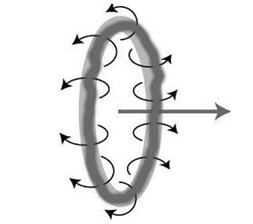
\includegraphics[width=0.4\textwidth]{graphics/theory/vortex-ring}
	\caption{Depiction of quantized vortex ring motion and induced velocity field. Source: Huang, Kerson, \textit{Quantum vorticity in nature}, arXiv.}
	\label{vortex-ring}
\end{figure}

More explicitly, it was shown \cite{donnelly_book} that in case of weak counterflow velocity $\vec{v}_{\text{ns}}$, the lifetime of vortex ring can be expressed as a simple relation:

\begin{equation}
\tau_{\text{ring}} = \frac{R_0}{2 \alpha \vert \vec{v}_{\text{ring}}(R_0)\vert}\,,
\label{ring-lifetime}
\end{equation}

where $R_0$ is the initial radius of created vortex ring.

By integrating the ring's motion equation from $R_0$ to $R(\tau) \approx a_0$ we obtain the distance travelled by the ring's center:

\begin{equation}
D_{\text{ring}} = \frac{\alpha}{1 - \alpha^{\prime}} (R_0 - a_0)
\label{ring-distance}
\end{equation}

Relations (\ref{ring-lifetime}) and (\ref{ring-distance}) are taken as a baseline in \textbf{Simulation} chapter.
\newpage

%%%%%%%%%%%%%%%%%%%%%%%%%%%%%%%%%%%%%%%%%%%%%%%%%%%%%%%%%%%%%%%%%%%%%%%%%%%%%%%%%%%%%%%%%%%%%%%%%%%%%%%%%%%%%%%%%%%%%%%%%%%%%%%%%%%%%%%%%%%%%%%%%%%%%%%%%%%%%%%%%%%%%%%%%%%%%%%%%%%%%%%%%%%%%%%%%%%%%%%%%%%%%%%%%%%%%%%%%%%%%%%%%%%%%%%%%%

{\Huge \bfseries Macroscopic view}
\addcontentsline{toc}{chapter}{Macroscopic model}
\vspace{0.3cm}

Besides NLSE and Vortex filament model, there is also a third, \textit{macroscopic} model in which the individual vortex lines are \textit{invisible} and the superfuid component of Helium-II is considered as a continuous flow of vortices. Many phenomena are similar to those in classical hydrodynamics (\textbf{Figure \ref{laminar-turbulent}}), but there emerge also new and very special type of events that can happen within superfluid Helium-II.

\begin{figure}[h]
	\centering
	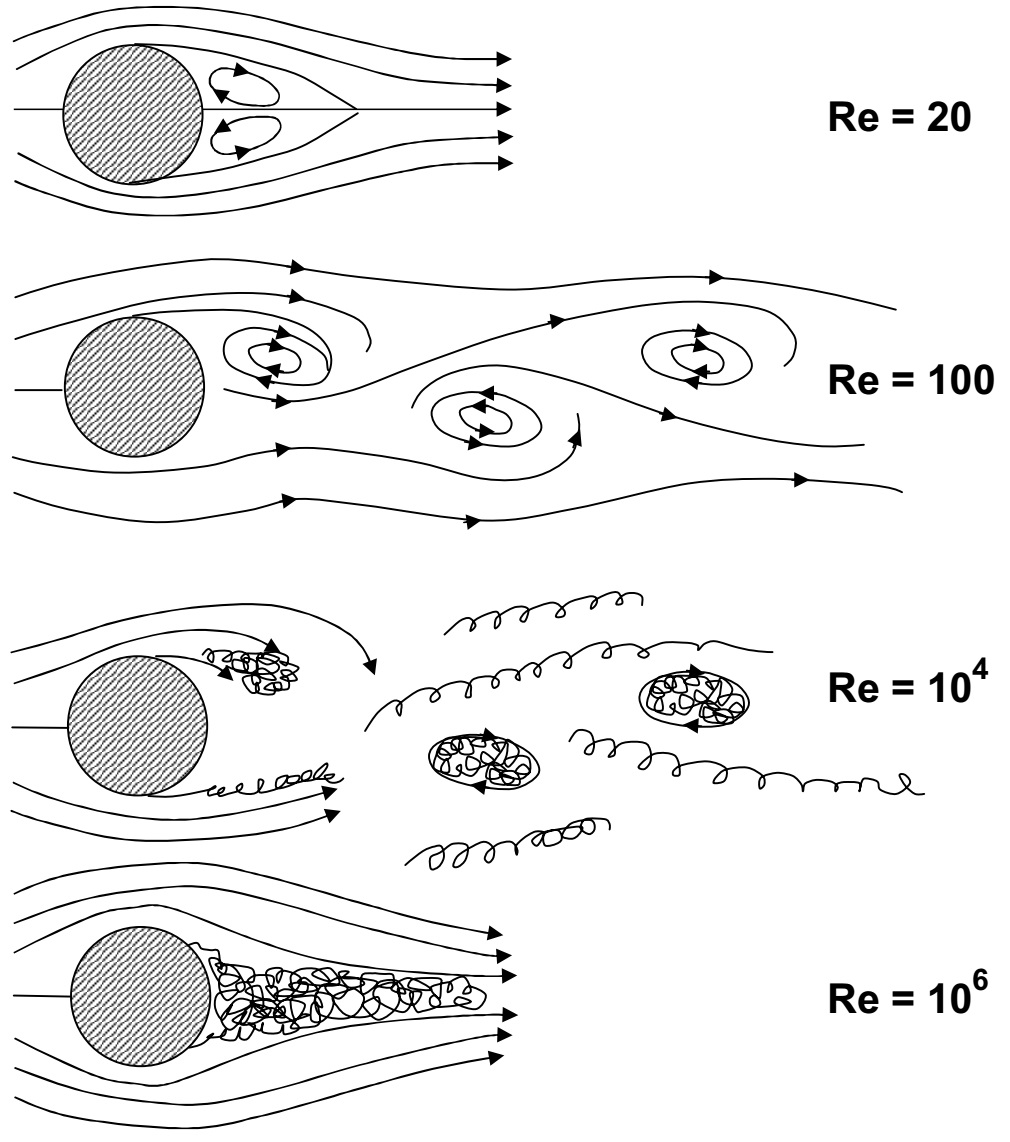
\includegraphics[width=0.5\textwidth]{graphics/theory/laminar-turbulent}
	\caption{Depiction of a classical steady flow for various Reynolds number values. Many phenomena of laminar, semi-turbulent and turbulent flows are visible in depcitions. Source: \cite{laminar-turbulence}}
	\label{laminar-turbulent}
\end{figure}

%%%%%%%%%%%%%%%%%%%%%%%%%%%%%%%%%%%%%%%%%%%%%%%%%%%%%%%%%%%%%%%%%%%%%%%%%%%%%%%%%%%%%%%%%%%%%%%%%%%%%%%%%%%%%%%%%%%%%%%%%%%%%%%%%%%%%%%%%%%%%%%%%%%%%%%%%%%%

\section{Hydrodynamics of superfluid}

Such macroscopic model is called the Hall-Vinen-Bekarevich-Khalatnikov (HVBK) model and provides a generalization of Landau's two-fluid model equations, including the presence of vortices. The superfluid is treated as a continuum and we can define a macroscopic superfluid vorticity $\vec{\Omega}_s$, despite the fact that, microscopically, the superfluid velocity field obeys $\nabla \times \vec{v}_s = \vec{0}$. The downside of this model is its assumption of spatially (not randomly) organized vortices. The common example is a rotating cylinder \cite{osborne}.\\

\newpage

The incompressible HVBK equations for normal component $\vec{v}_n (\vec{r}, t)$ and superfluid component $\vec{v}_s (\vec{r}, t)$, respectively, are \cite{barenghi}:

\begin{align}
\frac{\partial\vec{v}_n}{\partial t} + (\vec{v}_n\cdot \nabla)\vec{v}_n =& -\frac{1}{\rho} \nabla P - \frac{\rho_s}{\rho_n} S \nabla T + \frac{\eta}{\rho_n} \nabla^2 \vec{v}_n + \vec{F}_{ns}\,,
\label{motion_normal}\\
\frac{\partial\vec{v}_s}{\partial t} + (\vec{v}_s\cdot \nabla)\vec{v}_s =& -\frac{1}{\rho} \nabla P + S \nabla T + \vec{T} - \frac{\rho_n}{\rho} \vec{F}_{ns}\,,
\hspace{15mm}
\label{motion_super}
\end{align}

where we have defined:

\begin{equation}
\vec{F_{ns}} = \frac{B(T)}{2} \vec{\hat{\Omega}} \times [\vec{\hat{\Omega}}_s \times (\vec{v}_n - \vec{v}_s - \nu_s\nabla \times \vec{\hat{\Omega}})]
+ \frac{B^{\prime}(T)}{2} \vec{\Omega}_s \times (\vec{v}_n - \vec{v}_s - \nu_s\nabla \times \vec{\hat{\Omega}}_s)\,,
\end{equation}
\begin{equation}
\vec{\Omega}_s = \nabla \times \vec{v}_s\,,
\end{equation}
\begin{equation}
\vec{\hat{\Omega}}_s = \vec{\Omega}_s / \vert \vec{\Omega}_s \vert\,,
\end{equation}
\begin{equation}
\vec{T} = - \frac{\varkappa}{4\pi} \log(b_0 / a_0) \, \vec{\Omega}_s \times (\nabla \times \vec{\hat{\Omega}}_s)
\end{equation}

Here we can identify the quantities as $\vec{F_{ns}}$ (mutual friction force), $\vec{T}$ (vortex tension) and $\eta$ (viscosity parameter). Usually, $b_0$ is the intervortex spacing and can be estimated as $b_0 = (2\Omega_s \varkappa)^{-1/2}$. %Note that two-fluid equations (\ref{motion_normal}), (\ref{motion_super}) by Landau can be achieved by neglecting $\vec{F}$ and $\vec{T}$.
The HVBK equations have well-defined limiting cases:

\begin{itemize}
	\item $T \rightarrow T_{\lambda}$: In this case $\rho_s \rightarrow 0$ and the normal fluid motion equation (\ref{motion_normal}) becomes the classical Navier-Stokes equation with viscosity term.

	\item $T \rightarrow 0$: In this case $\rho_n \rightarrow 0$ and the superfluid motion equation (\ref{motion_super}) describes a pure (potential) superflow. Additionally, taking the classical limit ($\hbar \rightarrow 0$) would give us the pure Euler equation of inviscid fluid.
\end{itemize}

The HVBK model has been widely used with success to study the transition to classical or quantum turbulence, for estimations of critical Reynolds numbers and its temperature dependence.

\newpage

%%%%%%%%%%%%%%%%%%%%%%%%%%%%%%%%%%%%%%%%%%%%%%%%%%%%%%%%%%%%%%%%%%%%%%%%%%%%%%%%%%%%%%%%%%%%%%%%%%%%%%%%%%%%%%%%%%%%%%%%%%%%%%%%%%%%%%%%%%%%%%%%%%%%%%%%%%%%

\section{Dynamical similarity principle}

An important role in the behaviour of fluids is taken by the \textit{fluid dimensional numbers}, which are used for scalling of motion equations in fluid mechanics.

The principle of \textit{dynamical similarity} states that two flows of similar geometry have the same dynamical behaviour, if they can be characterised by the same set of suitable dimensionless parameters representing transport phenomena. In order to describe Helium-II with correct equations and with the most precision, we have to choose which dimensionless parameters are useful.

\begin{itemize}
	\item \underline{Knudsen number} (Kn): This number helps determine whether statistical mechanics or the continuum mechanics formulation of fluid should be used to model the system. Kn is defined as the ratio of the molecular mean free path $\lambda$ to a representative physical length scale $D$ (container size).\\
	If the temperature of Helium-II is set above $T > 1.0 \unit{K}$, there is a still sufficient amount of normal component and the mean free path of thermal excitations is much smaller, comparing it with container scale $\lambda \ll D$. In that case, continuum mechanics could be used as a macroscopic theory for superfluid Helium-II.

	However, if temperature is below $T < 0.6 \unit{K}$, the mean free path $\lambda$ becomes comparable with length scale $D$ and the continuum model starts to break down. Here, the system is rather described as a gas of thermal excitations.

	\item \underline{Weissenberg number} (Wi): This number relates the typical frequency of perturbations, $\omega$ , of the fluid with the characteristic time, $\tau$ that describes the relaxation of the fluid towards a thermodynamic equilibrium. The Weissenberg number is then given as a multiplication of oscillation frequency $\omega$ and the relaxation time $\tau$.\\
	Since the relaxation time of Helium-II is relatively small in temperatures above $T > 1\unit{K}$, then $\text{Wi} = \omega \tau \ll 1$, so Helium-II can be considered as a Newtonian fluid.

	Once again, if temperature is below $T < 0.6 \unit{K}$, relaxation time of thermal excitations rises rapidly, meaning $\text{Wi} \sim 1$, causing the excitations propagating ballistically.

	\item \underline{Reynolds number} (Re): Let's consider the continuum and newtonian assumptions ($\text{Kn} \ll 1$ and $\text{Wi} \ll 1$), so the fluid can be described by the raw form of Navier-Stokes (N-S) equation of motion. When we take into account also the incompressibility $\nabla \dotprod \vec{v} = \vec{0}$, the N-S for classical fluid reduces itself to its most simplest form.\\
	In case of stationary flow ($\partial \vec{v} / \partial t = \vec{0}$), N-S can be rewritten into a dimensionless form. Following these steps, there arises typical values of velocity $U$ and length scale $L$, at which there is the most significant change in velocity. Re can be expressed as a ratio of inertial and dissipative forces as $\text{Re} = U L \rho / \eta$, where $\eta$ is the dynamic viscosity of the flow field.\\
	The oscillatory case is described more in the next section.

\end{itemize}

The derivation of the \textit{dynamical similarity} phenomenon can be directly seen from inspection of the underlying motion equation (\ref{motion_normal}) with geometrically similar bodies. In the classical fluid dynamics, we use dynamical similarity and scaling arguments for expressing experimental data in terms of Reynolds numbers, drag coefficients, lift, and so on.

Alternatively, the dissipative forces may be described in terms of a dimensionless \textit{drag coefficient} $C_D$, representing the relation between \textit{drag force} $\vec{F}$ and fluid velocity $\vec{U}$, and usually takes the form:

$$
C_D \!\propto\! U^\alpha, \hspace{1cm}
\text{where}
\left\{
  \begin{array}{l l}
    \alpha=-1 & \quad \text{for laminar flow $\Re \in (0-10)$}\\
    \alpha=0 & \quad \text{for turbulent flow $\Re \in (10^3-10^5)$}
  \end{array}
\right.\,,
$$

where the first case ($C_D \propto 1/U$) represents the viscous skin friction anf the second case ($C_D \approx \text{const.}$) represents the pressu drag.\\
It is very common to plot experimentally measured dependence of drag coefficient $C_D$ against the Reynolds number, for various objects (sphere, disc, cylinder) past flow:

\begin{figure}[h]
	\centering
	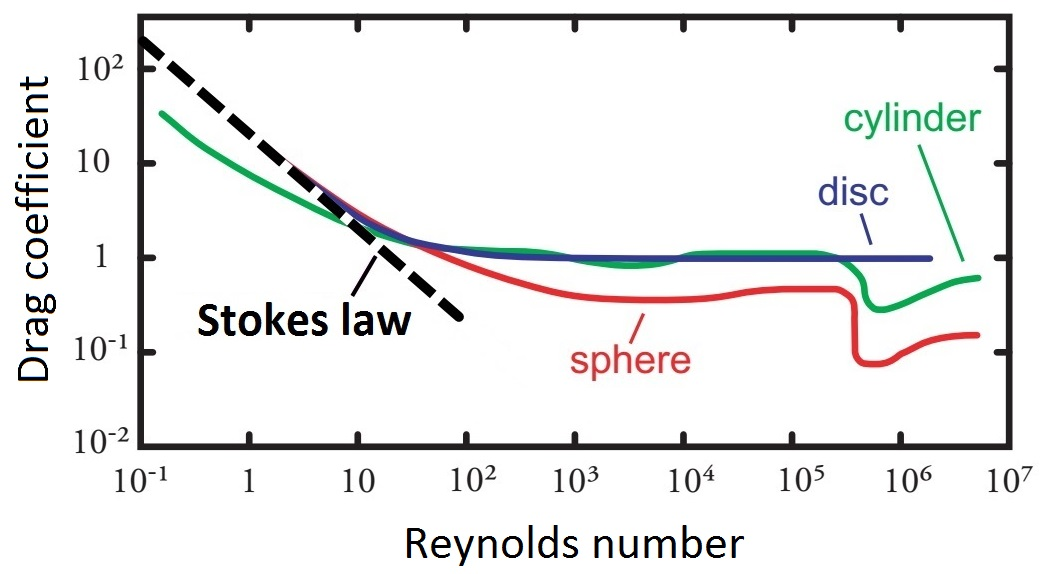
\includegraphics[width=0.7\textwidth]{graphics/theory/C-Re}
	\caption{Drag coefficients of different objects in a steady flow with changing Reynlods number. Blue line - thin disc, Green line - cylinder with drag crisis near $\Re \approx 10^6$, Red line - sphere with similar drag crisis as with cylinder, Black dashed line - laminar drag, where $C_D \propto \Re^{-1}$.}
	\label{C-Re}
\end{figure}

Dynamical similarity argument also leads to the existence of critical Reynolds number, at which the transition to turbulence in case of classical fluid occurs. Note that since superfluid Helium-II is composed of two fluids, the mentioned applies only to the normal component. The transition of superfluid component to quantum turbulence is described wider in next chapters

%%%%%%%%%%%%%%%%%%%%%%%%%%%%%%%%%%%%%%%%%%%%%%%%%%%%%%%%%%%%%%%%%%%%%%%%%%%%%%%%%%%%%%%%%%%%%%%%%%%%%%%%%%%%%%%%%%%%%%%%%%%%%%%%%%%%%%%%%%%%%%%%%%%%%%%%%%%%

\section{Oscillatory flows}

If a given body is oscillating in a classical viscous fluid, described by ordinary Navier-Stokes equation, there appears another characteristic lenght scale, identified by \cite{landau} as the \textit{viscous penetration depth}:

\begin{equation}
\delta(\omega) = \sqrt{\frac{2\eta}{\rho\omega}}\,,
\label{penetration}
\end{equation}

where $\omega$ is the angular frequency of oscilations.\\
To recognize correct characteristic length scale (whether it should be oscillating body dimension $D$ or penetration depth $\delta$), we calculate the ratio of time-dependent term $\partial \vec{v} / \partial t$ from N-S equation (\ref{motion_normal}) to the viscous term $\nabla^2 \vec{v}$. Hence, we define another dimensionless quantity, the \underline{Stokes number} $\beta$.
We calculate it \cite{stokes} as $\beta = \omega \rho D^2 / (\pi \eta)$, which can be reduced using (\ref{penetration}) to $\beta = D^2 / (\pi \delta^2)$.\\
From this, we call a situation as the \textit{high-frequency regime}, when $\delta \ll D$, so the Stokes values are $\beta \gg 1$.

\subsection*{Classical hydrodynamics}

To describe fully an oscillatory flow, the governing Navier-Stokes equations may be expressed in terms of dimensionless velocity $U$, time $T$ and positions $L$. The independent time scale is given by the angular frequency of oscillations $\omega$. Candidates for characteristic lenght scale $L$ may lead to the body size $D$, surface roughness, or the viscous penetration depth $\delta(\omega)$.

In the high frequency limit (directly from \ref{penetration}) $\omega \gg 2\eta / (\rho D^2)$, depending on body geometry, one can reach $\delta(\omega) \ll D$ and say that fluid oscillates in
high Stokes regime \cite{universal_scaling} with $\beta = D^2 / (\pi \delta^2) \gg 1 $. Also, when also the surface roughness exceeds $\delta$, the N-S equation may be expressed using only one dimensionless parameter: an \textit{oscillatory Reynolds number} $\Re_{\delta} = \delta U \rho / \eta$.

\subsection*{Superfluid Helium-II}

Assuming two independent velocity fields $\vec{v}_n (\vec{r}, t)$, $\vec{v}_s (\vec{r}, t)$ in superfluid Helium-II, the above thoughts are applicable for the oscillatory viscous flow of the normal component $\vec{v}_n$. We therefore define the high frequency limit for normal component as:

\begin{equation}
\delta_n = \sqrt{\frac{2\eta}{\rho_n\omega}}\,,
\hspace{1cm}
\text{Dn} = \frac{U \delta_n \rho_n}{\eta}
\label{donnelly}\,,
\end{equation}

We will call the oscillatory Reynolds number for normal component in superfluid Helium-II as a \textit{Donnelly number} (Dn, after Russell J. Donnelly, who as first came with this (\ref{donnelly}) idea.

At low velocities, below the critical thresholds to create either classical or quantum turbulence, the flow of the superfluid component is purely potential and the normal component exhibits laminar viscous flow.

If the typical body curvature is of order $1/D$, the surface may be described as if consisting of many planar elements. In this case it is shown \cite{universal_scaling} that we can write for the average dissipated energy:

\begin{equation}
\langle \dot{E} \rangle =
\frac{1}{2} \alpha \xi U_0^2 S_{eff} \sqrt{\frac{\eta \rho_n \omega}{2}}\,,
\label{energy_loss}
\end{equation}

where $U_0$ is the velocity amplitude, $S_{eff}$ the effective surface, $\alpha$ the mutual friction constant and $\xi$ the integral of velocity profile along the resonator. The total energy of an oscillator is given as $E = \xi m U_0^2 / 2$ and moreover, we define a fluidic quality factor $Q_f$ of an oscillator for a single oscillation as:

\begin{equation}
1 / Q_f = \frac{\langle \dot{E} \rangle}{\omega E} = \frac{\alpha \rho_n S_{eff} \delta_n}{2m}
\label{quality}
\end{equation}

From (\ref{energy_loss}), one can also derive the peak dissipative force (during a period of oscillation) and the dimensionless drag coefficient related to the normal component:

\begin{equation}
F_0 = \frac{2 \omega \langle \dot{E} \rangle}{U_0}
= \alpha \xi \omega S_{eff} U_0 \sqrt{\frac{\eta \rho_n \omega}{2}}
\hspace{5mm}
\rightarrow
\hspace{5mm}
C_D^{\,n} = \frac{2 F}{A \rho_n U_0^2} = \frac{2 S_{eff}}{A U_0} \sqrt{\frac{\eta \omega}{\rho_n}}\,,
\label{drag_normal}
\end{equation}

where $A$ is the cross-section of the body perpendicular to flow. According to dynamical similarity principle, the drag coefficient (\ref{drag_normal}) can be expressed as a function of the dimensionless Donnelly number (\ref{donnelly}):

\begin{equation}
C_D^{\,n} = \Phi / \text{Dn}\,,
\end{equation}

where number $\Phi$ is determined by the oscillating body geometry. Clearly, the laminar case of normal component is fully described by the hydrodynamic laws. In turbulent case, we expect a constant value for $C_D^{\,n}$ as long, as only normal component contributes to the drag force (no quantum turbulence).

\section{Quantum turbulence}

Turbulence of superfluid component can be viewed as a tangle of vortex lines. In this case quantized vortices can be nucleated either \textit{intrinsically} (such process requires critical velocities of order $10 \unit{m/s}$) or \textit{extrinsically}, by stretching and reconnections of seed vortex loops. The initial vortices in the extrinsical case are the remnant vortices, which always exist in macroscopic samples of Helium-II . In many types of flow the critical velocity for extrinsic vortex nucleation is observed to be in order $\sim\unit{cm/s}$.

The superfluid component becomes turbulent at some critical velocity $U_C$ and therefore, we expect an increase in drag coefficient $C_D$ much above the possible dependence caused by turbulence of normal component. The process of self-reconecting remnant vortices was well studied \cite{universal_scaling} and the related critical velocity is expected to scale as $U_C \propto \sqrt{\varkappa \omega}$, where $\varkappa$ is the circulation quantum. Hence, it is convenient to define a dimensionless velocity $\hat{U}$ with related drag coefficient $C_D^{\,s}$ as:

\begin{equation}
\hat{U} = U_0 / \sqrt{\varkappa \omega}
\hspace{5mm}
\rightarrow
\hspace{5mm}
C_D^{\,s} = \frac{2 F_0}{A \rho_s U_0^2} = \frac{2 F_0}{A \rho_s \varkappa \omega \hat{U}^2}\,,
\label{drag_super}
\end{equation}

In case of turbulent superfluid component with velocities sufficiently above critical values, we expect both component to be coupled due to the mutual friction. In this case, both components contribute to the pressure drag, and drag coefficient must be calculated classicaly as $C_D = 2F / (A\rho U^2)$. where $\rho$ is the total density of Helium-II.

\newpage

\subsection*{Ultra-low temperature regime}

In classical fluids, when the mean free path $\lambda$ of particles becomes comparable to a lenght scale $D$ of the system ($\text{Kn} \sim 1$), the continuum model of the fluid starts to break down and the system cannot longer be described by the Navier-Stokes equations. Similar arguments go when the angular frequency of oscillatory flow $\omega$ becomes comparable with the relaxation time $\tau$ of the fluid towards thermodynamic equilibrium ($\text{Wi} = \omega \tau \sim 1$).\\
Here, the system is described as a gas of thermal quasiparticles propagating
ballistically through a physical vacuum. Therefore, such system state is called as \textit{ballistic regime}.

In practice with superfluid Helium-II, such situation is usually reached by cooling fluid  down to ultra-low temperatures. Below $T < 1\unit{K}$, the normal component accounts for less than $1\%$ of the total density, but required cooling to obtain ballistic regime (\textbf{Figure (\ref{ballistic})}) is below $T < 0.6\unit{K}$ (here the Helium-II is better described as a gas of thermal quasiparticles than a fluid).

\begin{figure}[h]
	\centering
	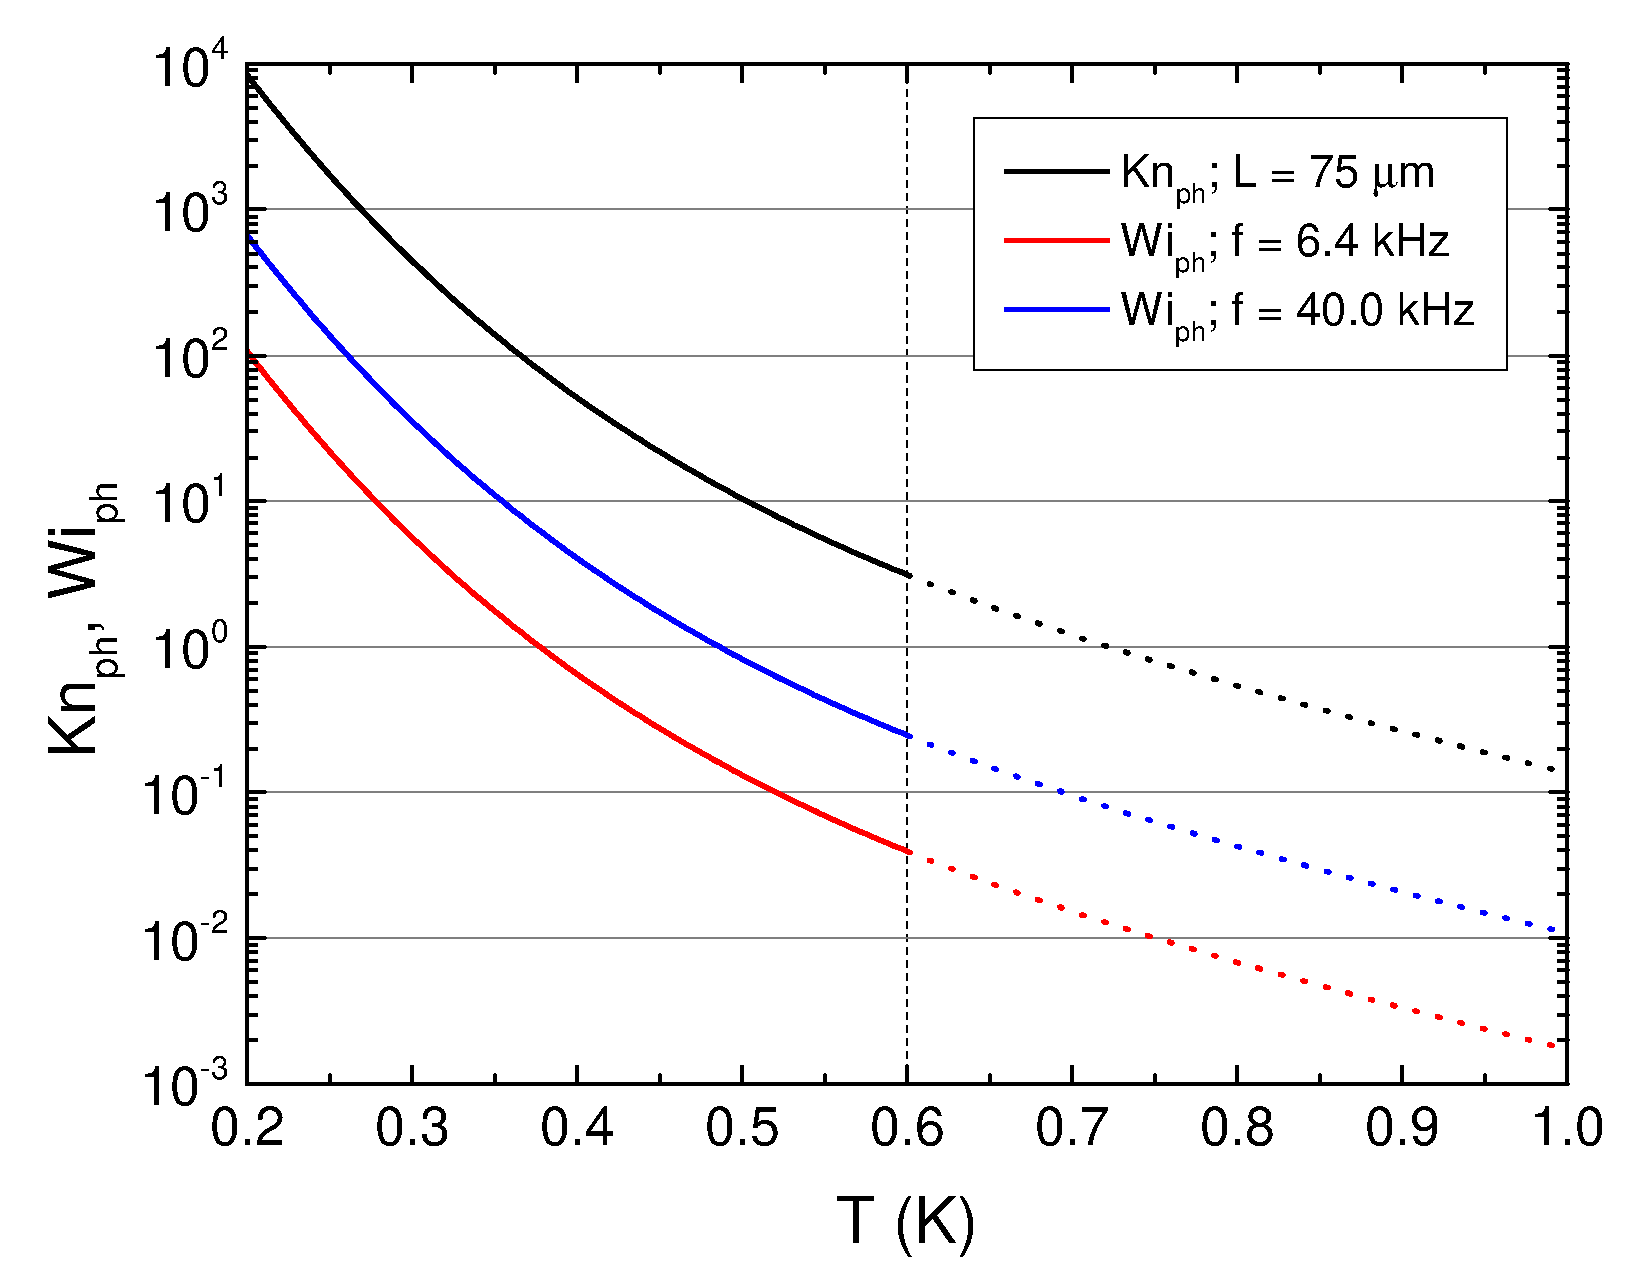
\includegraphics[width=0.7\textwidth]{graphics/theory/ballistic}
	\caption{Phonon Knudsen number and Weissenberg numbers plotted against temperature for different oscillators. The dashed line separates the interval $T < 0.6\unit{K}$, where the ballistic regime takes a place. Source: \cite{universal_scaling}}
	\label{ballistic}
\end{figure}

\newpage

\subsection*{Universal scaling}

A study was conducted in order to solve the Stokes' second problem with an oscillating plane in viscous fluid, using pure Boltzmann kinetic equation. This solution is used to derive a universality relation valid in the high frequency limit (with no turbulence present) across both Newtonian and non-Newtonian regimes of the fluid. Using scaling function $f(\omega \tau)$, the authors derived \cite{universal_scaling} the relation for the quality factor:

\begin{equation}
1 / Q_f = \frac{\alpha S_{eff}}{m} \sqrt{\frac{\eta \rho_n}{2\omega}} f(\text{Wi})
\end{equation}

In \textbf{Results} we use this form of universality scaling for comparison against experimental data collected in temperature ranges $T < 0.6\unit{K}$ or $T > 1\unit{K}$.

\subsection*{Multiple critical velocites}

Here is briefly commented the transition to quantum turbulence regime observed at very low temperatures ($T \ll 1\unit{K}$). A couple of experimental studies in milliKelvin temperatures reported \cite{crit-velocity} the existence of more critical velocities related with superfluid component flow within single experiment:

\begin{itemize}
	\item \underline{First critical velocity} is related to the formation of pinned vortex loops at the surface of oscillating body - possibly forming a thin layer with different hydrodynamic behaviour which increases the effective mass of the oscillating object. Such critical velocity is hard to observe at higher than ultra-low temperatures.

	\item \underline{Second critical velocity} is a consequence of vortex rings escaping from the oscillator body into the superfluid bulk and eventually forming a vortex tangle. Here the sudden raise of drag is observed, usually with hysteresis effect.

	\item \underline{Third critical velocity} is the highest critical velocity which can be observed. The origin of this velocity is linked to the development of larger quantized vortex structures, which in larger scale start to mimic the classical turbulence. Such velocity is in order $\approx \unit{m/s}$ and moreover, very likely screened by the influence of the normal component turbulence. Therefore, not likely reachable within experiments reported in this Rhesis.
\end{itemize}

% When both velocities of Helium-II are high enough, we expect the turbulent regime on both sides to be coupled due to mutual friction and contributing to the drag. In such situation, we are forced to use classical hydrodynamic metrics: drag coefficient $C_D = 2F / (A\rho U^2)$ and Donnelly number $D = U \delta / \nu$. Recent researches also hint that both classical turbulent and quantum turbulent regimes can exist separately with low interaction.
%
% Note that all presented approches are only approximate, since they are neglecting flows near the oscillating body, evaporation processes, sound emissions and other corner-case effects.

% \section{Second sound}
%
% Ordinary sound (the wave of density $\rho$ and pressure $P$) in Helium-II is called \textit{first sound}. In such process, temperature $T$ and entropy $S$ is conserved and $\vec{v}_n$ and $\vec{v}_s$ oscillate in phase with each other ($\vec{v}_n(t) \approx \vec{v}_s(t)$). On the contrary, by combination of two-fluid motion and continuity equations, one obtains the wave equation also for the temperature $T$ and entropy $S$. In such case the velocities obey an antiphase oscillation ($\rho_n(t) \vec{v}_n(t) \approx - \rho_s(t) \vec{v}_s(t)$) and remains $\rho$ and $P$ constant.
%
% \begin{figure}[h]
% 	\centering
% 	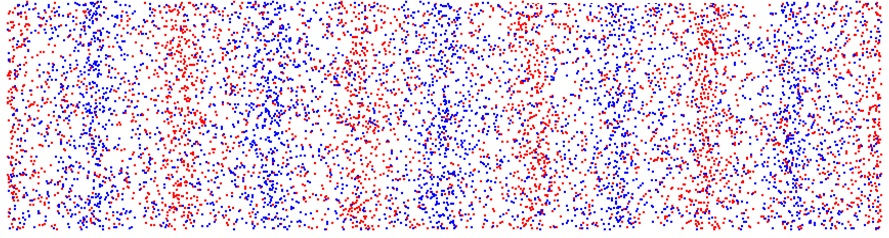
\includegraphics[width=0.99\textwidth]{graphics/theory/ss_1}
% 	\caption{here will come more proper picture}
% 	\label{ss_1}
% \end{figure}
%
% \begin{figure}[h]
% 	\centering
% 	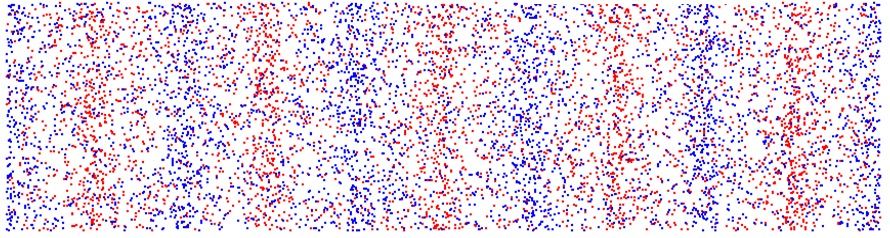
\includegraphics[width=0.99\textwidth]{graphics/theory/ss_2}
% 	\caption{here will come more proper picture}
% 	\label{ss_2}
% \end{figure}
%
% In early Vinen's observations, the exponentially damped velocity of second sound wave, propagating through two-fluid medium, was derived from motion equations:
%
% \begin{equation}
% \vec{v}_{\ind{ns}} \propto e^{-\alpha \vert \vec{r} \vert} \vec{\hat{e}}_{\vec{r}}(\vec{k},\vec{r},\omega,t)\,,
% \end{equation}
%
% where $\alpha$ is the attenuation coefficient. When considering homogeneous chaotic distribution of vortex tangle, one can also derive the formula for the attenuation factor:
%
% \begin{equation}
% \alpha = \frac{B\kappa L}{6 \vert \vec{c}_2\vert}
% \label{alpha_mean}\,,
% \end{equation}
%
% where $B$ is the first mutual friction parameter and $\vec{c_2}$ is the initial second sound velocity. This velocity was experimentally examined and there was found a plateau near the value $20 \unit{m/s}$, which is desirable during experiments (stability against small temperature changes):
%
% \begin{figure}[h]
% 	\centering
% 	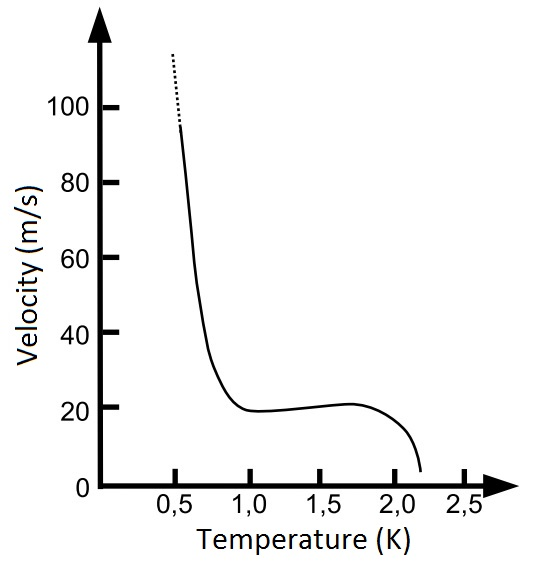
\includegraphics[width=0.4\textwidth]{graphics/theory/ss_velocity}
% 	\caption{velocity of the second sound with temperature}
% 	\label{ss_velocity}
% \end{figure}
%
% In this work, the phenomenon of second sound attenuation is used for detection of quantized vortices, which naturally appear within Helium-II. There is written much more about the method itself within the Experimental Approach part.

\newpage

%\chapter{Experimental Approach}

The experiments presented here were conducted in Prague and Lancaster independently. There are many experimental ways how to launch the production of quantum turbulence: by an oscillating objects (wires, the tuning forks, oscillating discs, etc.) or by a \textit{coflow} and \textit{counterflow} techniques.

In our investigation, we used the tuning fork oscillator, driven by alternating source Agilent A33220 and measured by SR830 amplifying lock-in. We measured both the in-phase and anti-phase componentes of signals. Results from other oscillators' measurements are included in this Thesis, however, not performed by the Thesis author.

\section{Apparatus}

All the measurements were performed in a helium cryostat (\textbf{Figure \ref{cryostat}}), cooled down to the desired temperatures using a rotary and Roots pump, and stabilized (with errors of a few mK) either manually or using the temperature controller. The working temperatures are from a wide range from a little above $T_{\lambda}$ to the lowest (experimentally) possible one $T_{min} \approx 1.3\unit{K}$. We also added series of measuremens from area far above $T_{\lambda}$, when $T = 3000\unit{K}$ to be confident about the hydrodynamical regime. The range $(1.3\unit{K} - 2.17\unit{K})$ allows access to most of the two-fluid regime.

\begin{figure}[h]
	\centering
	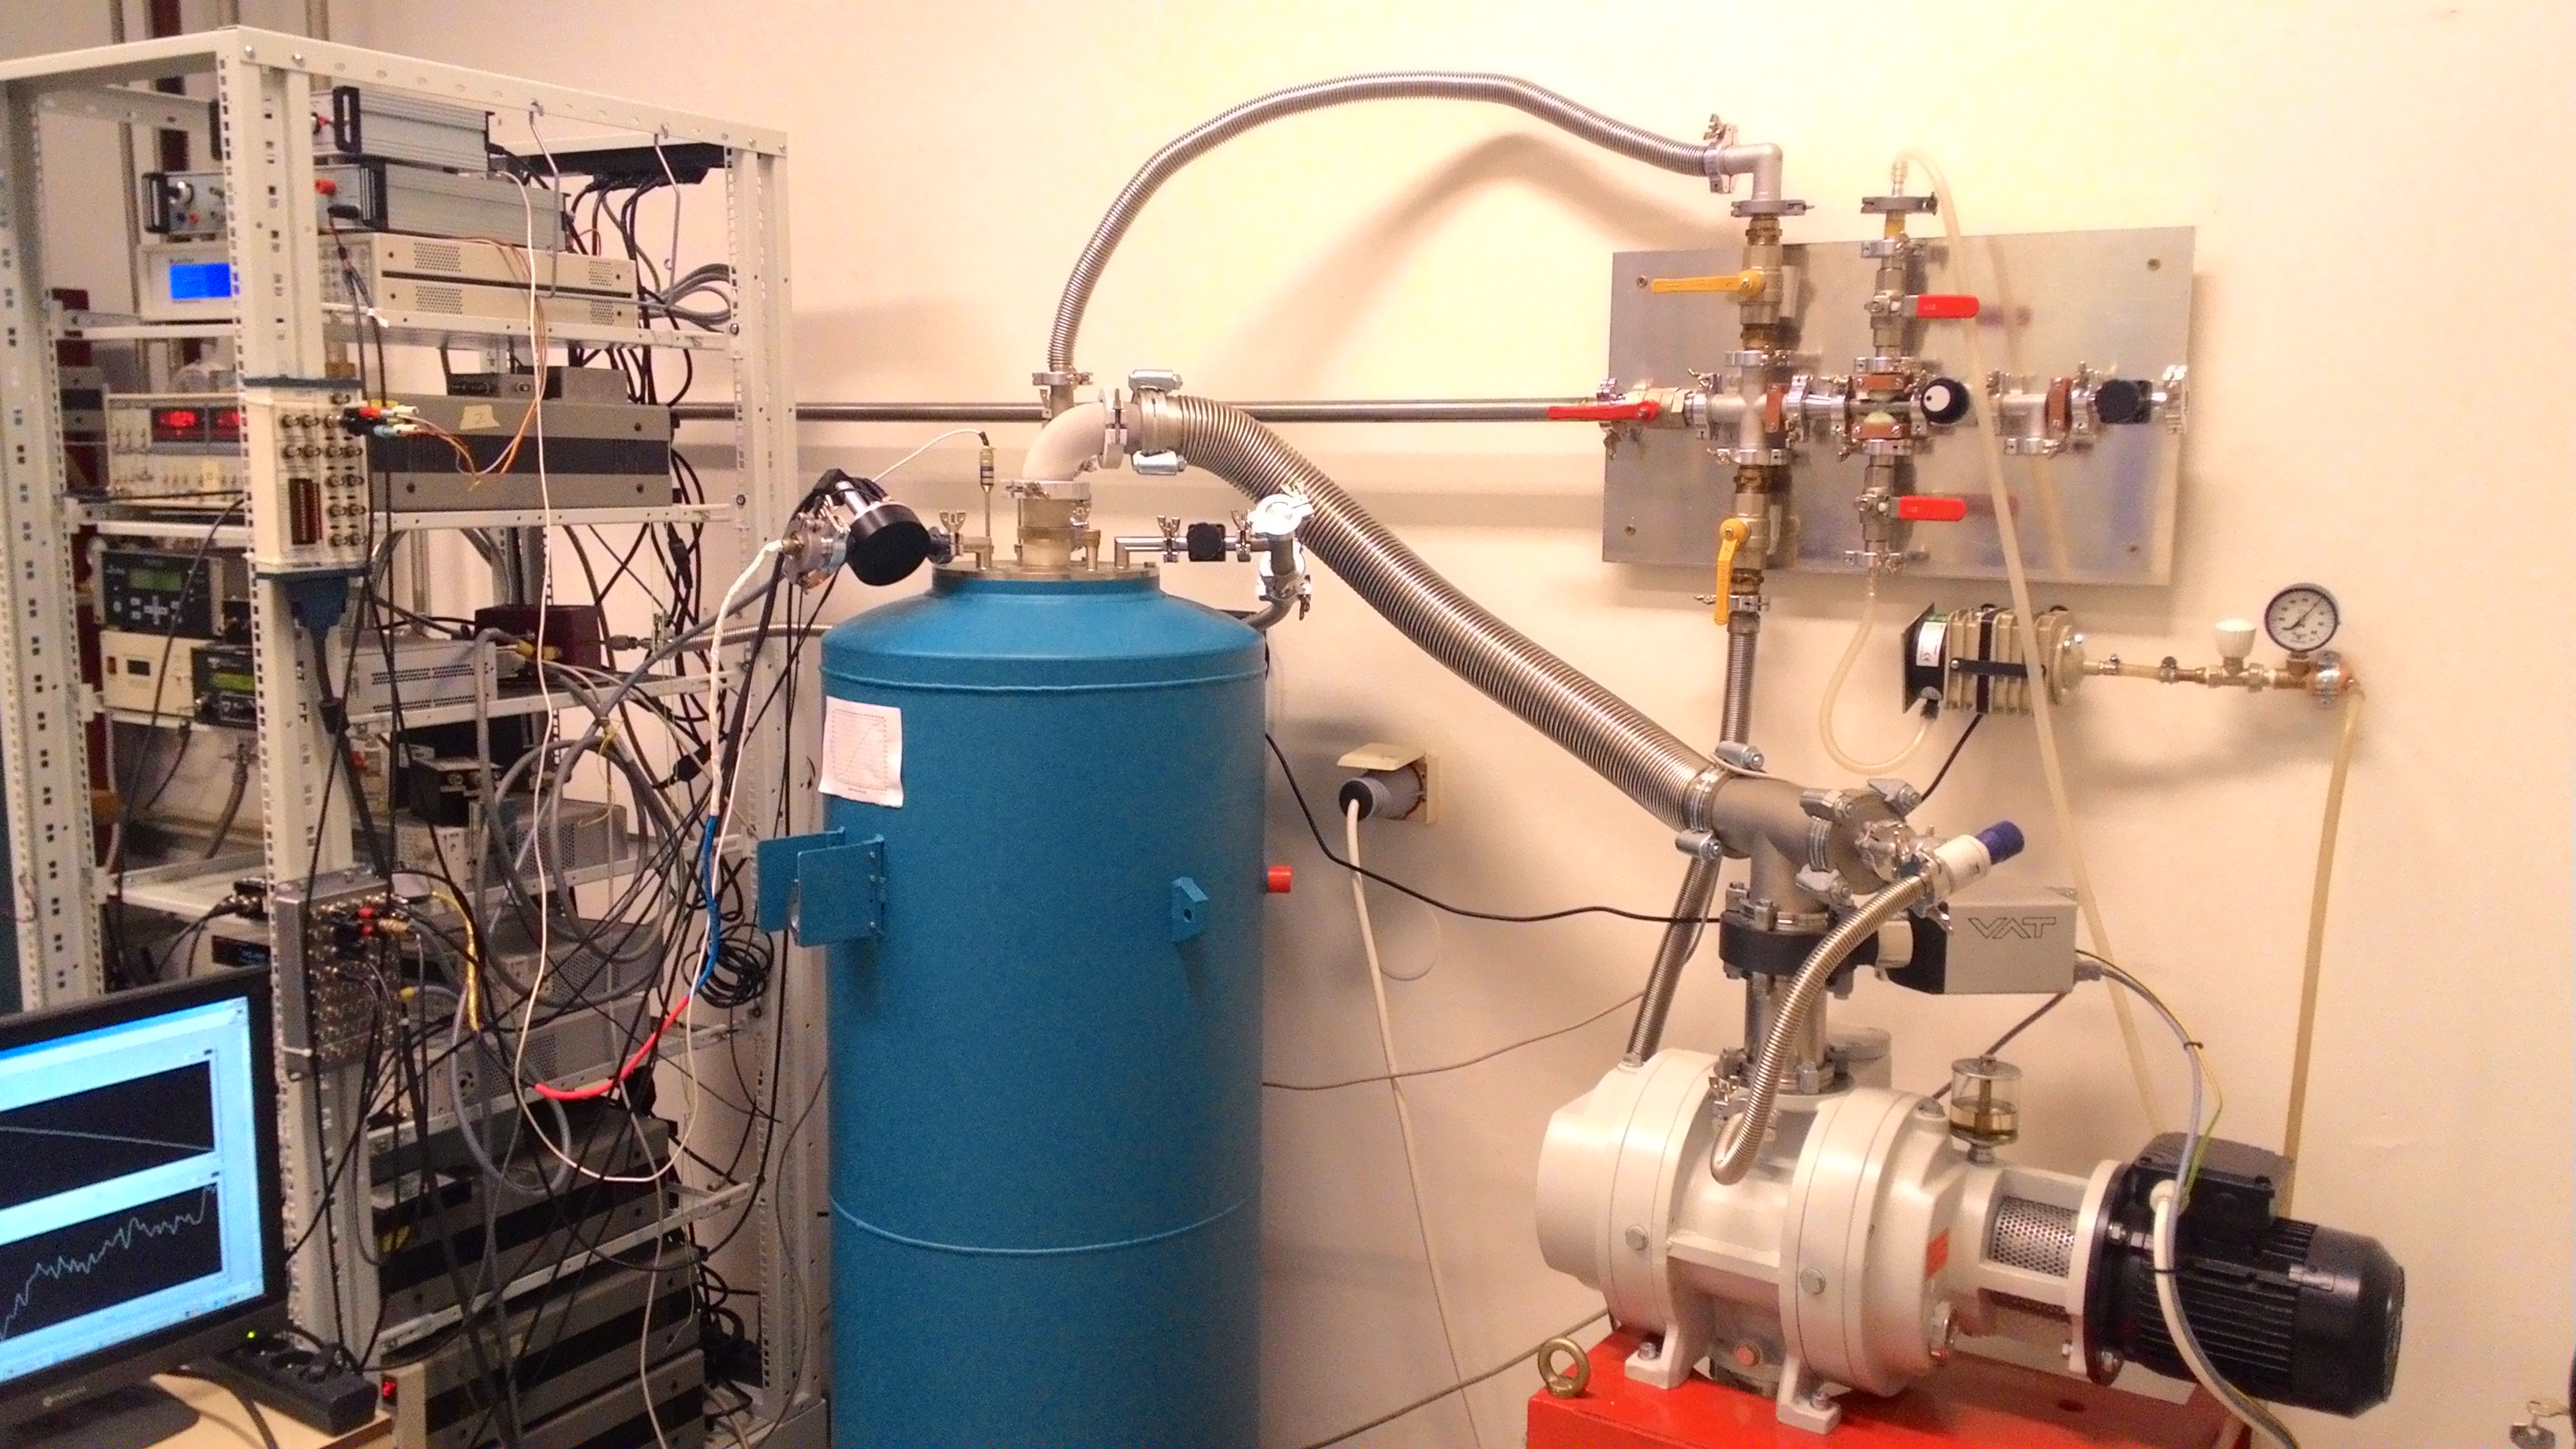
\includegraphics[width=0.8\textwidth]{graphics/exp/apparatus}
	\caption{A photograph of the experimental setup. From left: source generators, lock-in, cryostat, pipe system for emerging gas, Roots pump. Source: \cite{bakalaris}}
	\label{cryostat}
\end{figure}

\newpage

Measurements at temperatures $T < 0.6\unit{K}$ temperatures in the ballistic regime were performed on a Leiden Cryogenics MNK126-400 dilution refrigerator with a base temperature below $10 \unit{mK}$. These sub-Kelvin measurement description is not included in this Thesis. However, refrigerator results are used in \textbf{Results} part to demonstrate the uniform scaling theory.

Resonator was attached at the bottom (\textbf{Figure \ref{resonator}}) of the \textit{insert} - a large metalllic construction holding all mezsuring micro-devices. Insert serves as an vertical injection to the cryostat, filled continuously with helium from above. Therefore, resonator was place at the bottom, to ensure that it is submerged as long as possible.

\begin{figure}[h]
	\centering
	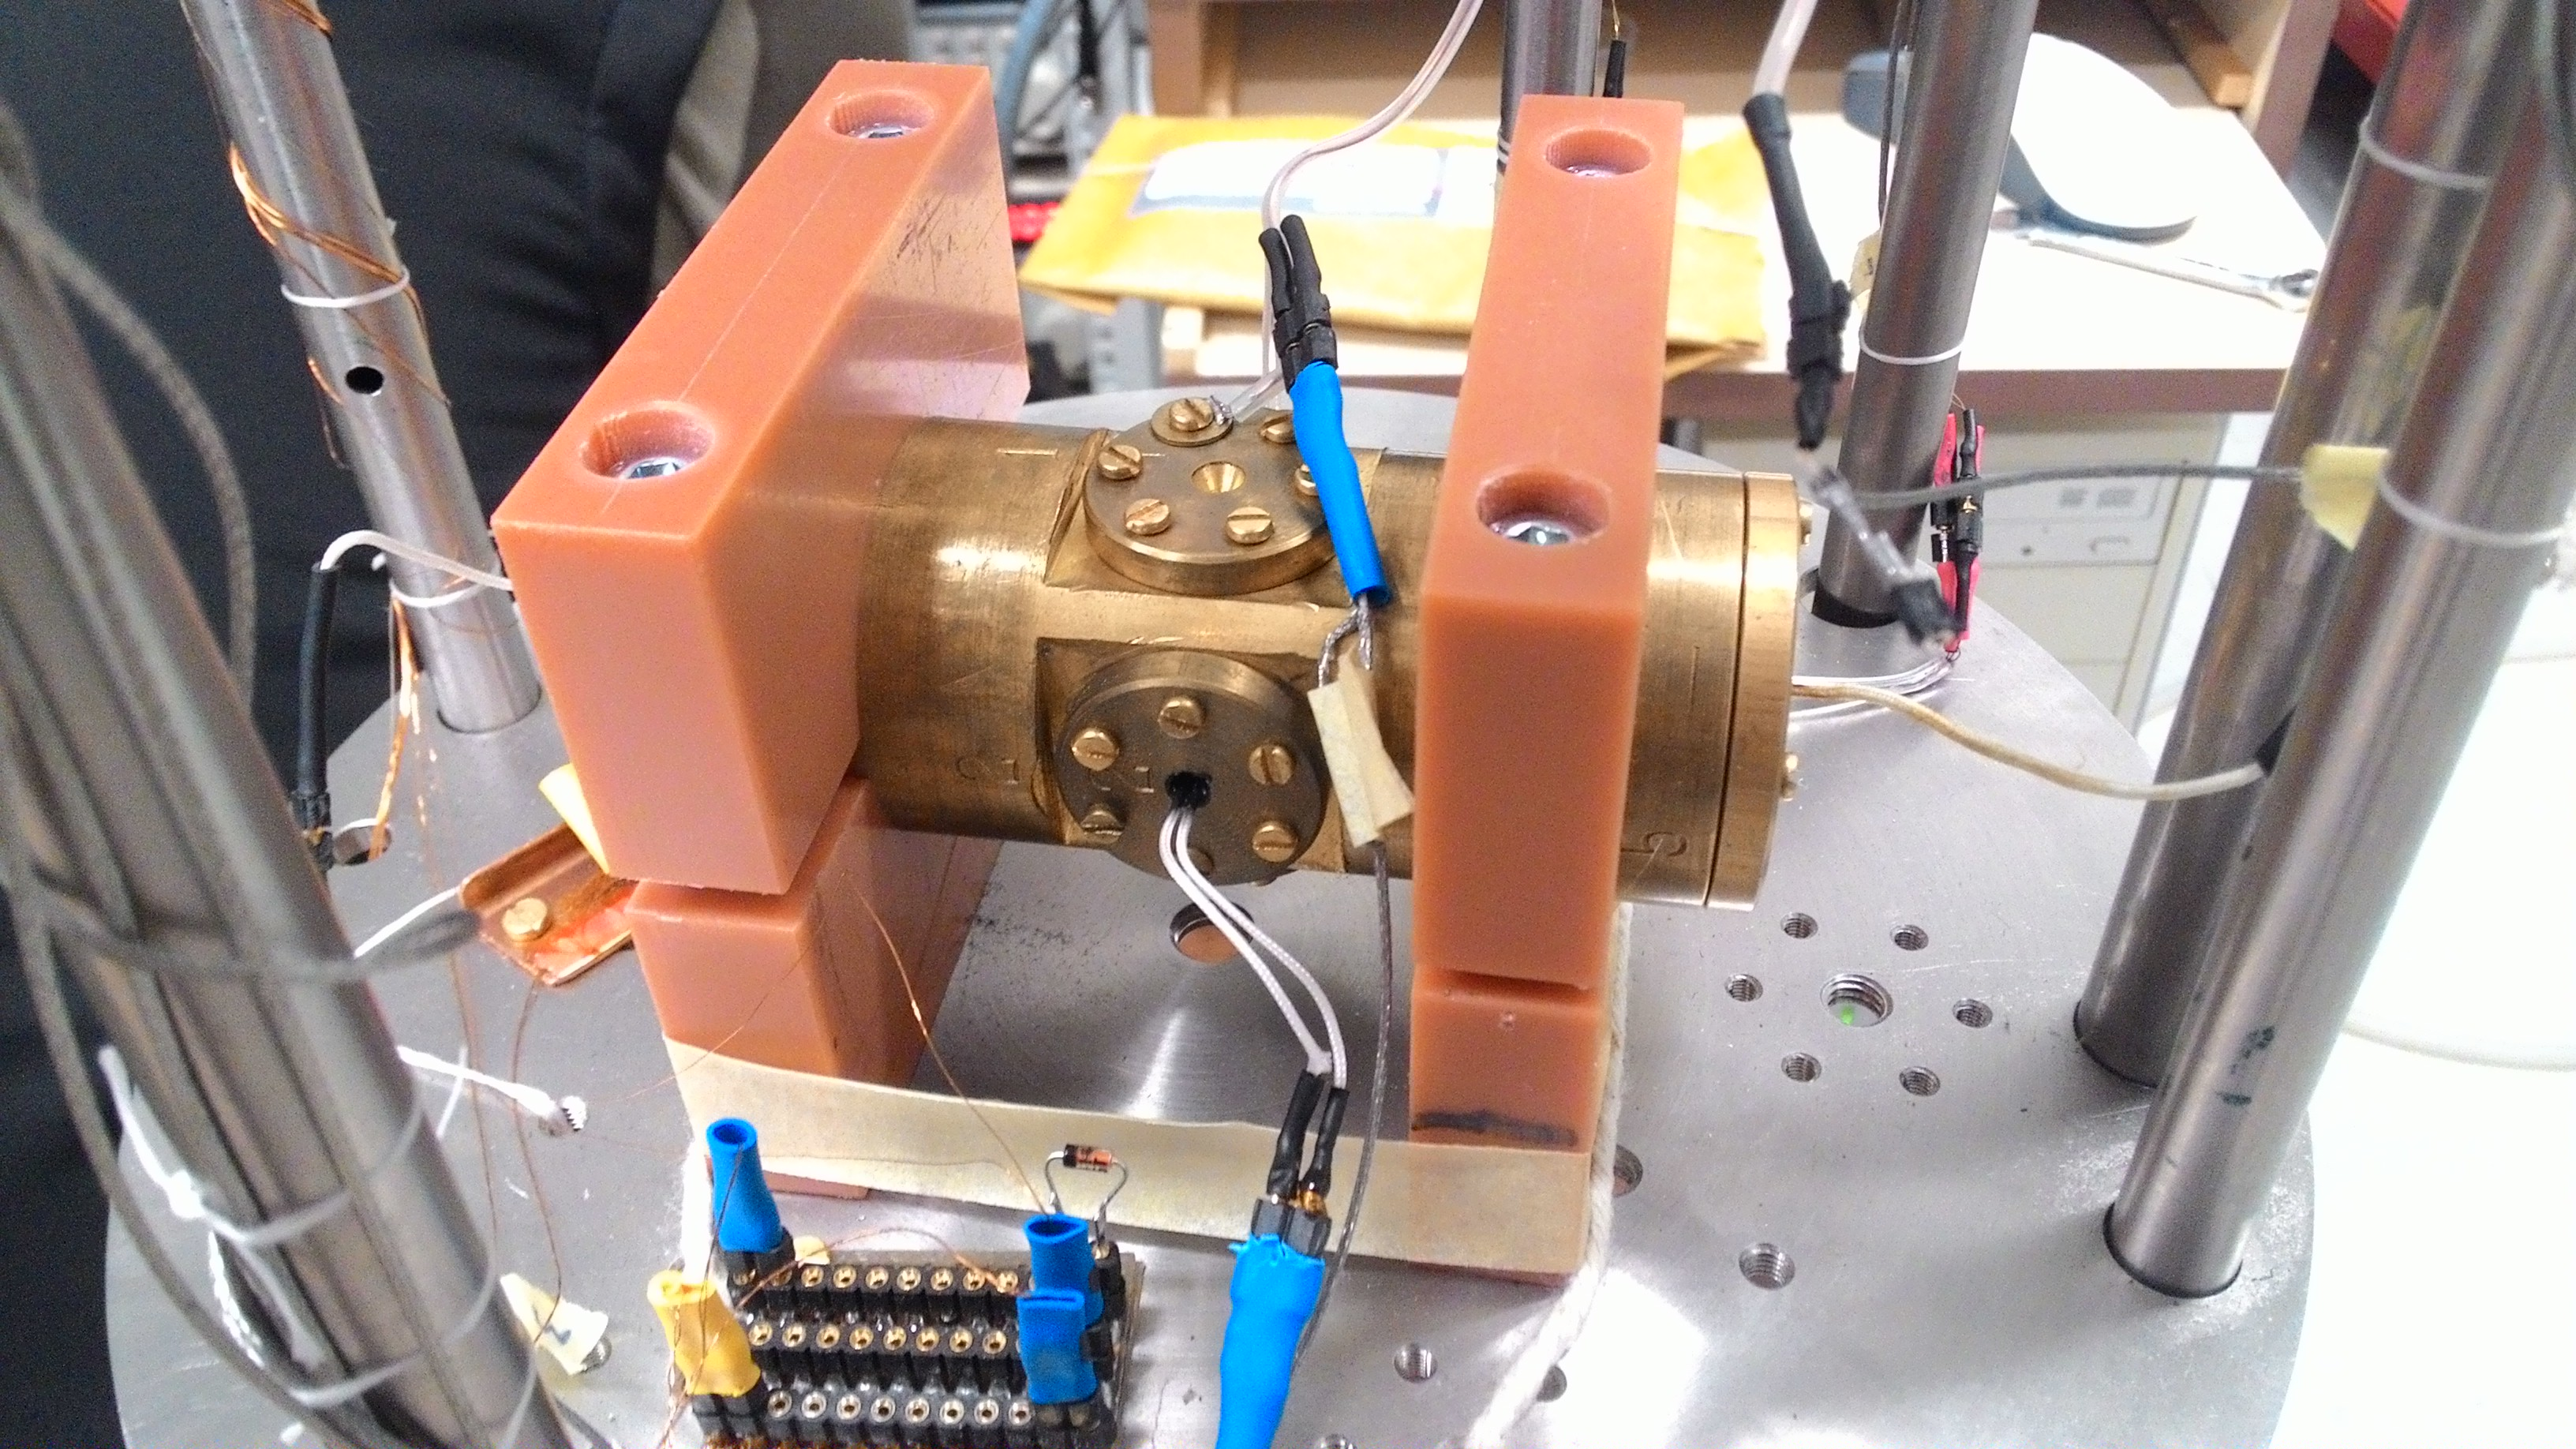
\includegraphics[width=0.8\textwidth]{graphics/exp/chamber}
	\caption{A photograph of the resonator attached at the bottom of metallic insert. Source: \cite{bakalaris}}
	\label{resonator}
\end{figure}

To obtain the best results at low temperatures both in vacuum and superfluid helium, the Prague cell containing the oscillators was flushed repeatedly with dry nitrogen gas prior to cooling. Each time it was pumped down below $\approx 10^{-5}\unit{mbar}$ using a turbomolecular pump.

After the last evacuation (to $\approx 10^{-6}\unit{mbar}$), the direct connection was closed off. With reasonable confidence that no helium ices could form on the resonators at low temperature, we strated ti fill the cell with pure superfluid 4-Helium. At this point, all calibrations of thermometers and resonators were made.


\newpage

\section{Resonators}

In this part we briefly describe the principles of small oscillating resonators used in Helium-II experiments.

\subsection*{Vibrating Wire}

Vibrating wire resonator consists of a semi-circular loop of wire inserted to a vertical magnetic field $\vec{B}$, as shown in \textbf{Figure \ref{wire}}. As we turn on the alternating current flux $\vec{j} \propto e^{i\omega t}$ inside the wire, these currents forces the wire to oscillate due to Lorentz force $\vec{F}_L \propto \vec{j} \times \vec{B} $. As the wire is moves through the field, the Faraday voltage is induced of magnitude \cite{universal_scaling}:

\begin{equation}
V = - \frac{\text{d} (\vec{B} \dotprod \vec{S})}{\text{d} t}
\sim \frac{\pi}{4} BDU\,,
\end{equation}

where $\vec{S}$ is the area vector, enclosed by the wire loop and $D$ is the distance between wire's legs. Experimentally used magnetic fields were in range $(170 \pm 10) \unit{mT}$.

\begin{figure}[h]
	\centering
	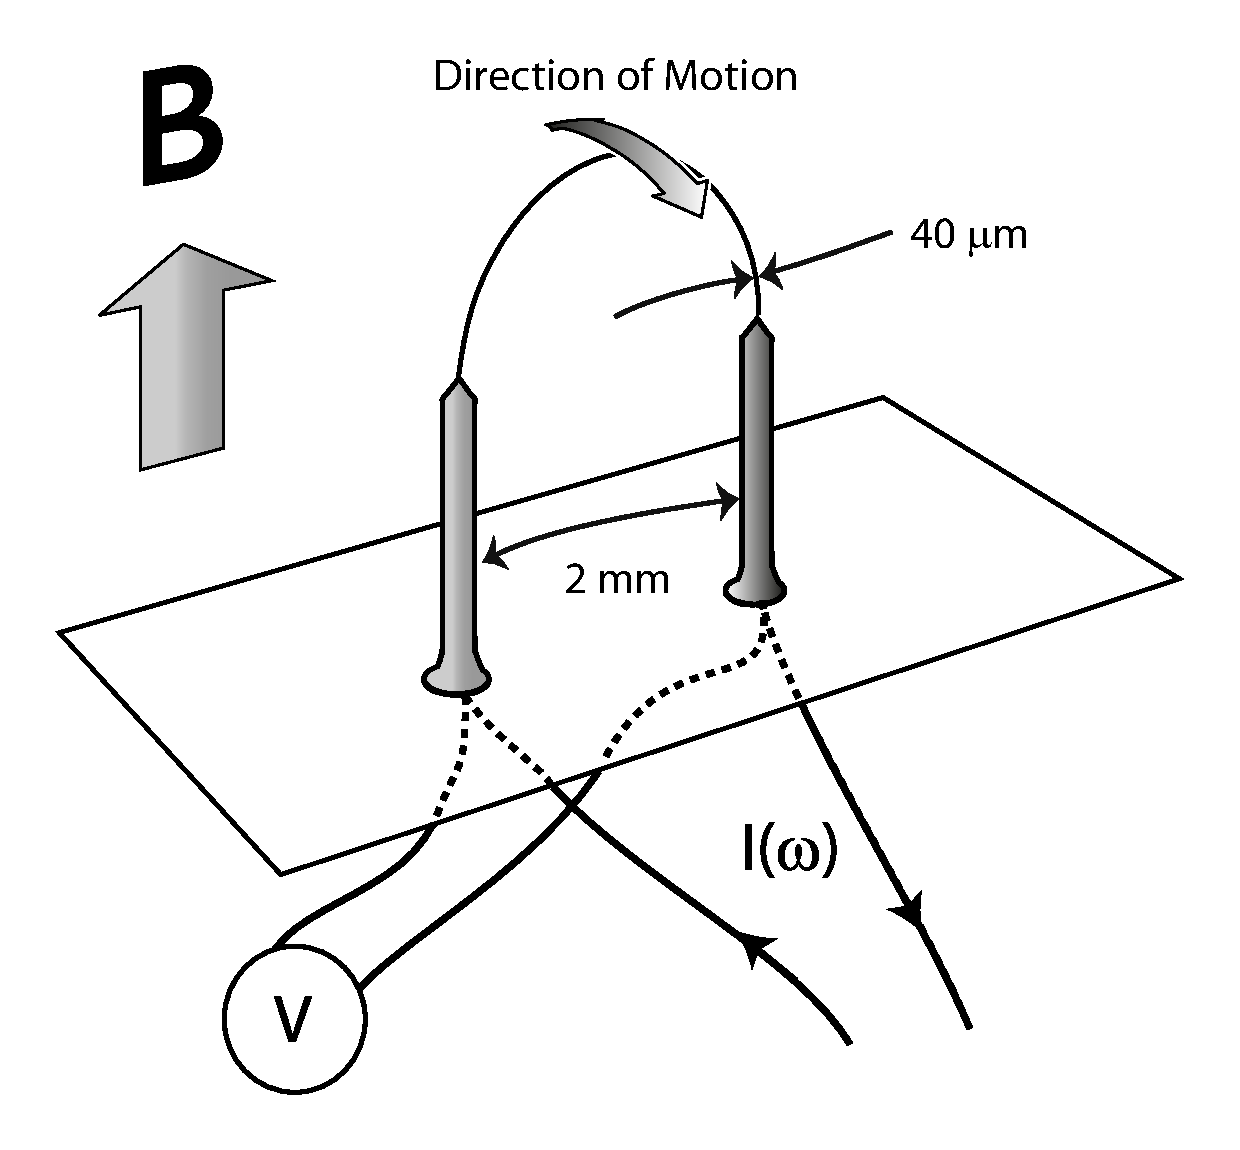
\includegraphics[width=0.5\textwidth]{graphics/exp/wire}
	\caption{Schematic diagram of the vibrating wire resonator. Source: \cite{universal_scaling}}
	\label{wire}
\end{figure}

\newpage

\subsection*{Tuning Fork}

Quartz tuning forks (TF) are commercial piezoelectric oscillators with a well-calibrated resonant frequency. They are usually used as frequency standards in watches or as force sensors in microscopes. Also, TFs have started to be widely used in cryogenic Helium II experiments.

In our experimental work, we used the fork of following dimensions: prongs length $ \mathcal{L} = 3.50\unit{mm} $, prongs width (perpendicular to the fork plane) $ \mathcal{W}=75 \mu\unit{m} $, thickness $ \mathcal{T}=90\mu\text{m} $ prongs interdistance $ \mathcal{D}=90\mu\text{m} $.\\
A sketch of the fork architecture is depicted in \textbf{Figure \ref{fork}}:

\begin{figure}[h]
	\centering
	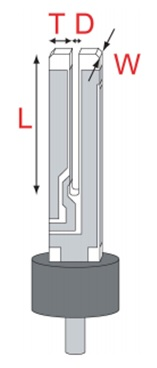
\includegraphics[width=0.25\textwidth]{graphics/exp/quartz}
	\caption{Schematic diagram of the quartz tuning fork. Source: \cite{bakalaris}}
	\label{fork}
\end{figure}

There are several achievable resonant modes at which the fork can oscillate. We chose to work with the \textit{fundamental} one at $f_0 = 6.7 \unit{kHz}$ and with the first \textit{overtone} one at $f_1 = 41 \unit{kHz}$.\\
The fork is driven by applying an alternate voltage $V(t) \propto e^{i\omega t}$ from a generator to the metalic plates (deposited on fork surface). The piezoelectric effect causes a tension resulting in a force, which is proportional to the applied voltage. In fundamental mode, the fork exhibits an anti-phase oscillating motion of its prongs with a single node. In case of overtone, there would be just two nodes. The fork's flex induces a piezoelectric current $I(t)$ about which is shown its proportionality to the velocity $U(t)$.

\newpage

The conversion relations between applied $V(t)$, measured $I(t)$ and mechanical properties $F(t)$, $U(t)$ are given \cite{fork} as:

\begin{equation}
F(t) = \frac{1}{2} a_{rmf} V(t)\,,
\hspace{1cm}
U(t) = \frac{I(t)}{a_{rmf}}\,,
\end{equation}

where $a_{rmf}$ is the so-called \textit{fork constant}. This constant can be derived from a fork's geometry, material and an oscillation mode. Usually the formula for this constant is given by a deflection measurement:

\begin{equation}
a_{rmf} = \sqrt{4\pi m_{eff} \Delta f \frac{I}{V}}\,,
\end{equation}

where $m_{eff} = TWL\rho_q /4$ ($\rho_q$ as the quartz density) is the fork's effective mass and $\Delta f$ is the measured peak width from the fequency-sweep deflection measurement. In our case we used fork with the effective mass and fork constants for fundamental and overtone mode of following values:

\begin{equation}
m_{eff} = 1.52 \times 10^{-2} \mu\unit{g}\,,
\hspace{1cm}
a_0 = 0.3 \mu\unit{Cm}^{-1}\,,
\hspace{1cm}
a_1 = 1.41 \mu\unit{Cm}^{-1}
\end{equation}

The measurement scheme for the Prague experiment with tuning fork is shown in \textbf{Figure \ref{setup}}. The arrangement of other experiments in Lancaster were slightly more complex, but similar.

\begin{figure}[h]
	\centering
	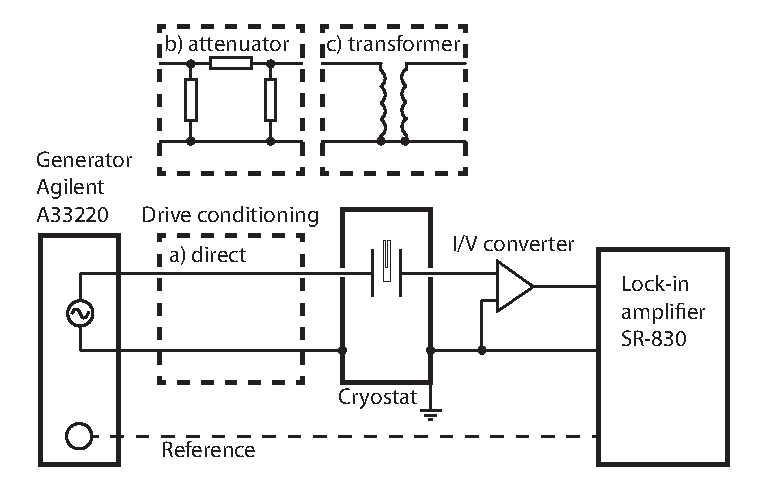
\includegraphics[width=0.6\textwidth]{graphics/exp/fork_setup}
	\caption{Diagram of the measurement scheme used in Prague. To achieve the full range of velocities, the applied voltage was either (a) directly fed to the tuning fork, (b) attenuated by one or more inline attenuators, or (c) amplified by a transformer. The transformer’s output was constantly monitored. Source: \cite{multiple-vels}}
	\label{setup}
\end{figure}

\newpage

\subsection*{Oscillating Disc}

The torsional oscillator consists of a $50 \mu\unit{m}$ wire  with a glass disc fixed to
the wire at its midpoint. The disc is $1\unit{mm}$ thick with a diameter of $40\unit{mm}$. A schematic picture is showed in \textbf{Figure \ref{disc}}.\\
Sixteen black marks around the circumference of the disc are used to determine the deflection and angular velocity of the disc from recorded video sequences.

\begin{figure}[h]
	\centering
	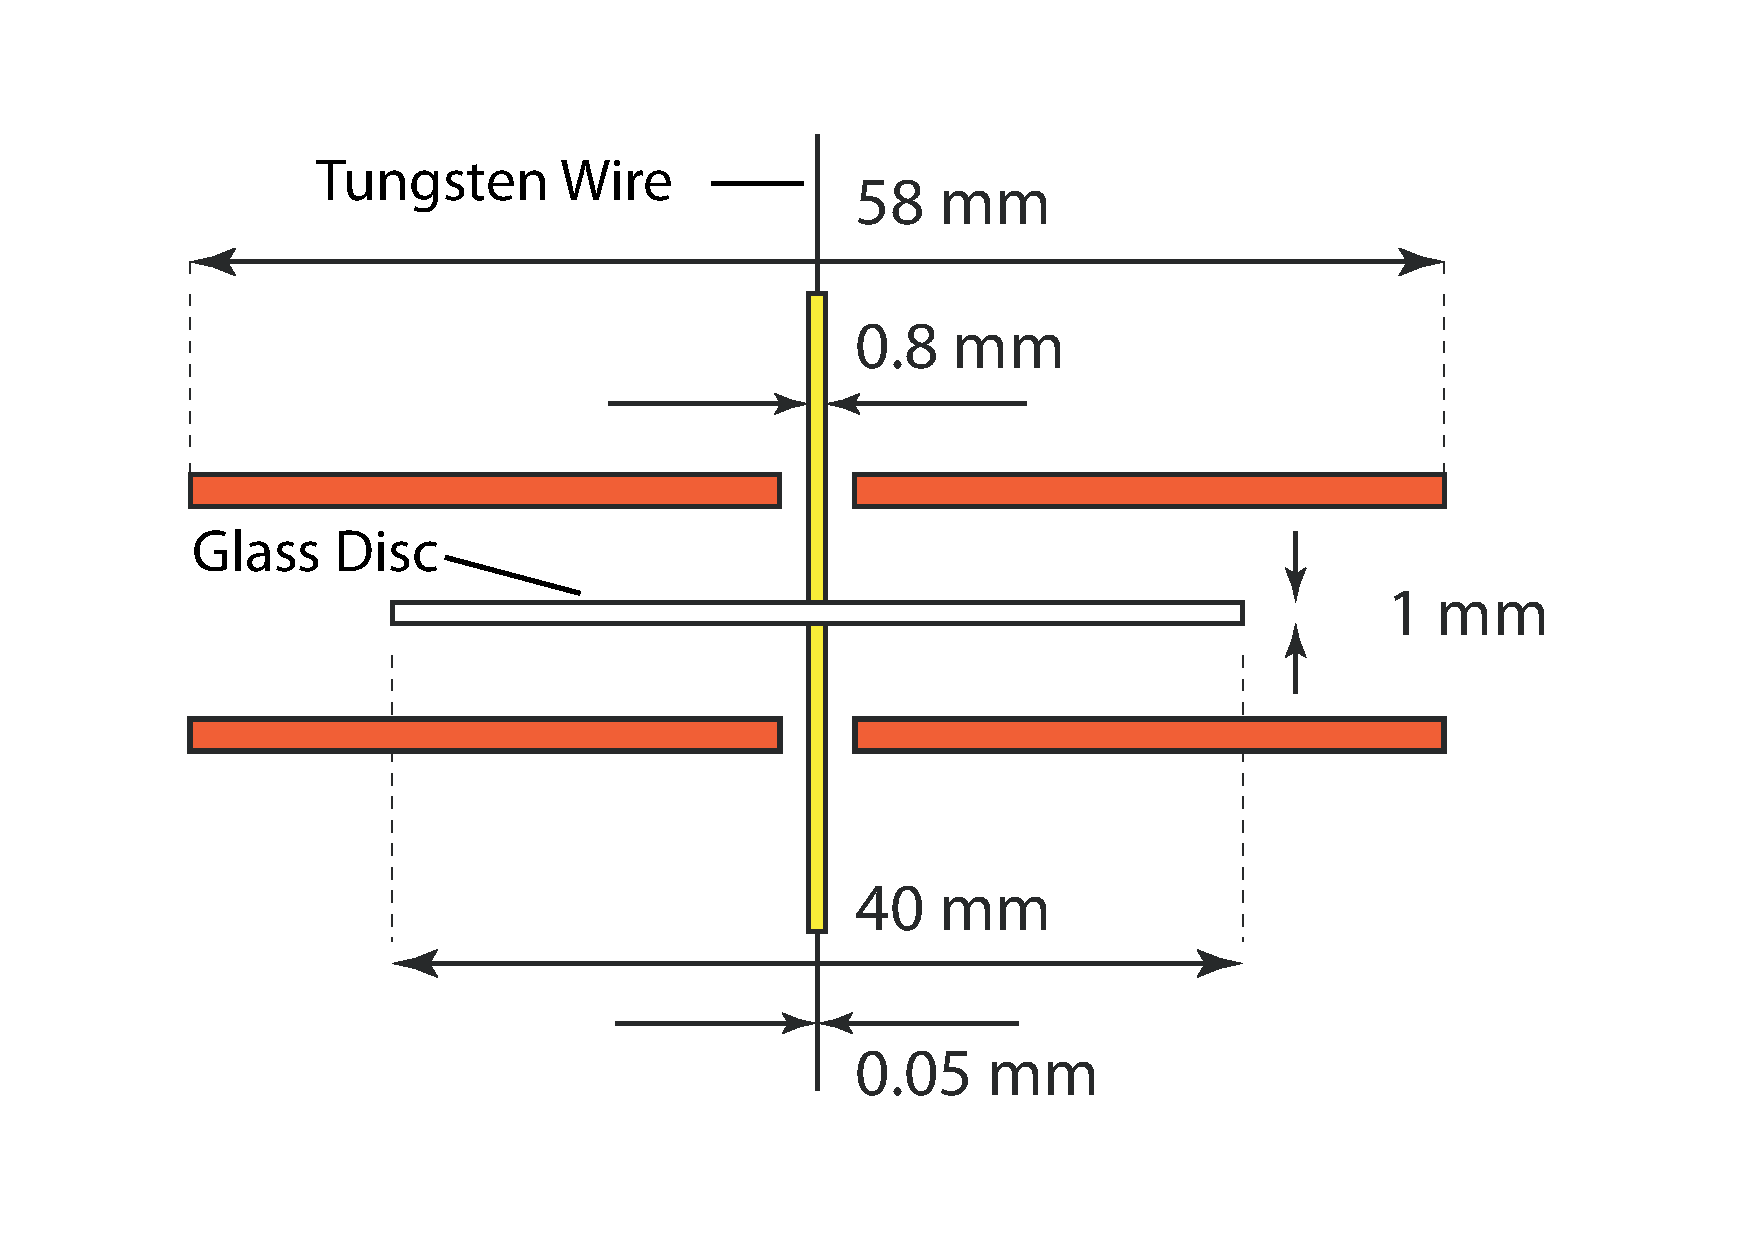
\includegraphics[width=0.7\textwidth]{graphics/exp/disc}
	\caption{Schematic diagram of the torsionally oscilating disc. Source: \cite{universal_scaling}}
	\label{disc}
\end{figure}

The raw data is in the form of video recordings of the disc motion and fairly complex post-processing method was required to extract quantities. The optical distortion from the lenses and the curved walls of the cryostat are negligible.

\newpage

%\newpage

\chapter{Results}

Here we present the experimental data obtained from the measurements of quantum turbulence. The tuning fork has been immersed in superfluid $\He$ and forced to oscillate at two, geometrically different (in the sense of different velocity profile along the fork's prongs) modes - \textit{fundamental} $ [6380\unit{Hz}] $ and \textit{overtone} $ [40\,000\unit{Hz}] $.

The first part of this chapter is focused on the measurement of vortex line density $ L $ (total length of vortices in unit volume) using the second sound attenuation technique. We will try to find the conditions for production of quantized vortices and also, quantify their amount.

In the second part we will work only with the tuning fork via the applied voltage amplitudes and its current responses. Using the scaled drag coefficient and oscillatory Reynolds number, we will be able to estimate when the drag force acting on the tuning fork becomes non-linear with velocity. This event is a distinct sign of the flow pattern changing from simple laminar flow of the normal component and purely potential flow of the superfluid component, to something more complex involving some form of classical and/or quantum turbulence.

Overall we worked at seven selected temperatures in the two-fluid regime, when both superfluid and normal component amounts are considerable: $ 1.35\unit{K} $, $ 1.55\unit{K} $, $ 1.65\unit{K} $, $ 1.80\unit{K} $, $ 1.95\unit{K} $, $ 2.05\unit{K} $, $ 2.15\unit{K} $.  {\sffamily\textbf{Figure 3.1}} shows the time trace of the temperature inside the cell. Temperatures below $\approx 1.30\unit{K} $ were not stable, so the lowest fixed value was set to $ 1.35\unit{K} $.  


\begin{figure}[h!]
	\centering
	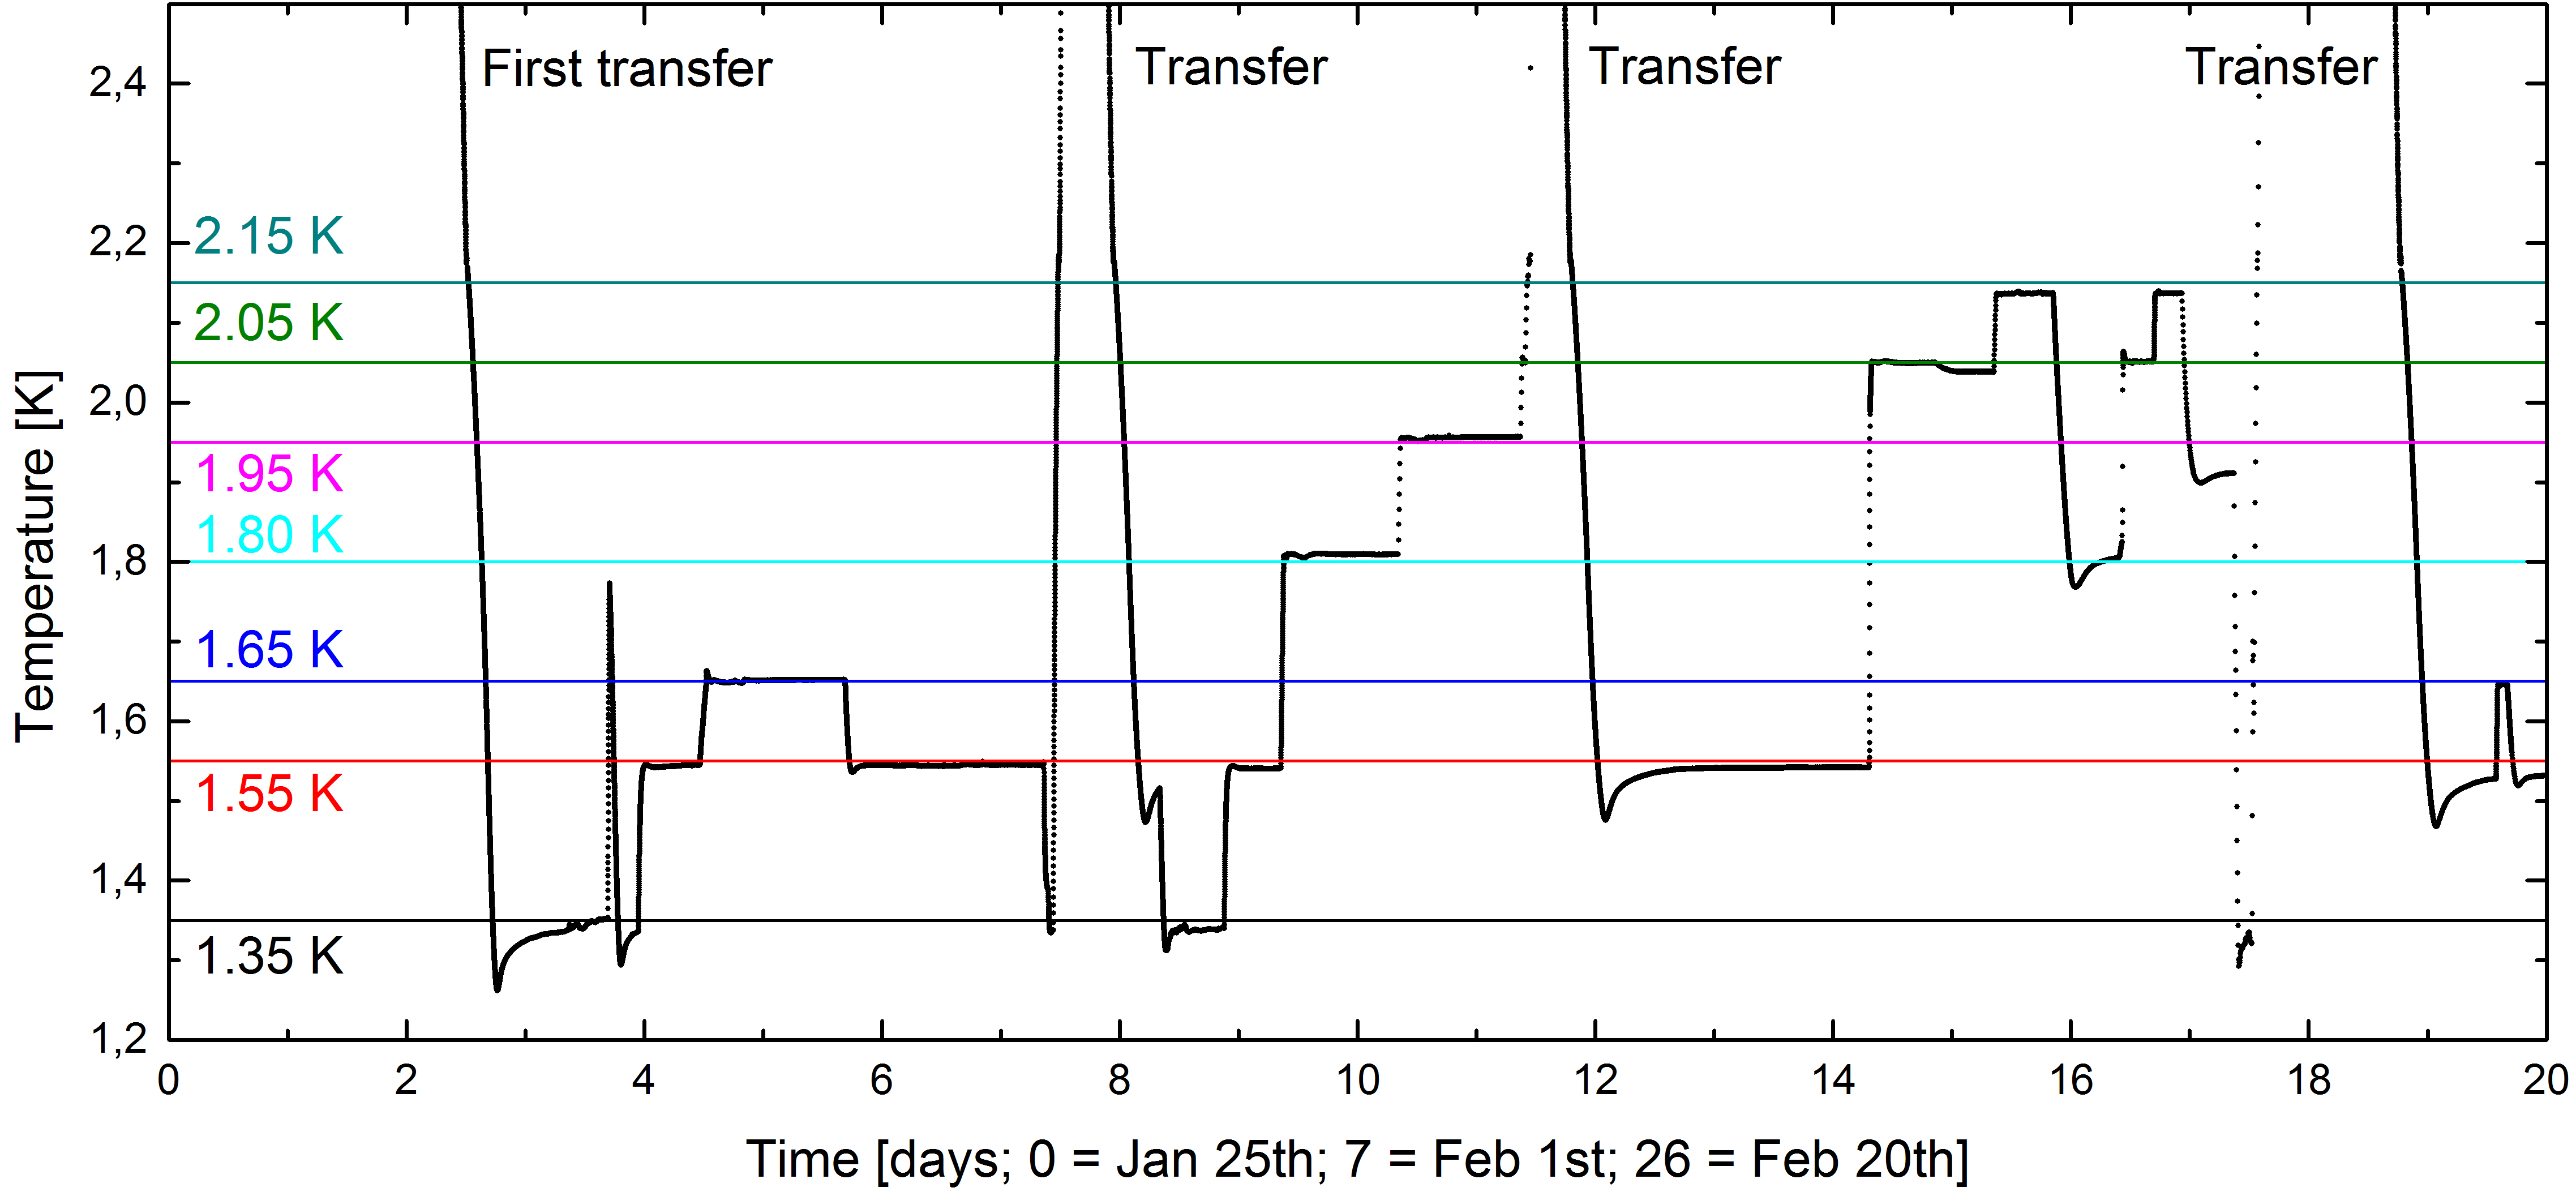
\includegraphics[width=1\textwidth]{graphs/diary}
	\caption{Record of the temperature inside the cryostat. Due to strong evaporation of superfluid helium and relatively long durations of the measurements at each temperature, we had to refill the cryostat three times. Unfortunately, this may have caused some unsystematic behaviour of the tuning fork that manifested after the first refill on Day 8, see the text for details.}
\end{figure}

Due to the prolonged experimental times, we had to refill helium three times, which has likely contributed to unsystematic behaviour of the tuning fork. The fork has yielded different results at the same temperature before and after transfers, especially the refill on Day 8. The data presented in this Thesis should thus be considered as if consisting of two separate categories of measurements: (i) temperatures $ 1.35\unit{K} $, $ 1.55\unit{K} $, $ 1.65\unit{K} $ investigated before Day 8; and (ii) remaining higher temperatures investigated after said transfer. Where we had the choice, we chose to present data measured before the transfer, as we believe that these better reflect the actual properties of the tuning fork and are more useful for comparison (e.g. they compare better with Ref. \cite{lancaster}). Similar effects in terms of different behaviour after the refilling have been observed with other oscillators such as vibrating wires \cite{history}.

We believe that the most likely scenario is that during the transfer and subsequent cooling, some small amount of air entered into the helium bath, solidified, and despite the protection offered by the resonator body, some bits of frozen air found their way towards the surface of the fork and were deposited there. Consequently, the altered tuning fork geometry could have affected the helium flow, especially the exact moment when the drag force becomes non-linear due to a flow instability. While this unfortunate event means that we are, in principle, working with two different oscillators rather than the exact same tuning fork at all of the investigated temperatures, we believe that the vortex line density measurements correlated with the drag forces acting on the tuning fork still provide very interesting results and are highly valuable not only as a basis for further studies and improvements, but also directly, as a study of oscillatory flows in superfluid helium (regardless of the exact geometry of the vibrating object).


\section{Measurement of Vortex Line Density}

It has already been shown that an object oscillating with sufficient velocity can produce quantized vortices in superfluid helium. For this purpose, we used the tuning fork mounted in the second sound resonator. Our measurement protocol is given in the following steps:

\begin{itemize}
	\item[1)] First, after the desired temperature in the cryostat has been reached, we run the frequency sweep on tuning fork and second sound independently. The tuning fork frequency sweeps are repeated at different drive levels. This gives us the necessary information about the resonance frequencies and widths.
	
	\item[2)] Next we set up the second sound sensors in constant drive mode at its fundamental resonance and allow up to 3 minutes for stabilization.
	
	\item[3)] When this time has passed, we also run the tuning fork in constant drive mode at its resonance (fundamental or overtone) with a given voltage amplitude $ U_0 $ for 3 minutes.
	
	\item[4)] The tuning fork is subsequently turned off and the second sound is again left to stabilize for 2 minutes.

	\item[5)] The values of $ A $ and $ A_0 $ were taken as averages of the periods when the tuning fork was on and off (cutting the transients), respectively (see {\sffamily\textbf{Figure 3.2}}).
\end{itemize}


\begin{figure}[h!]
\centering
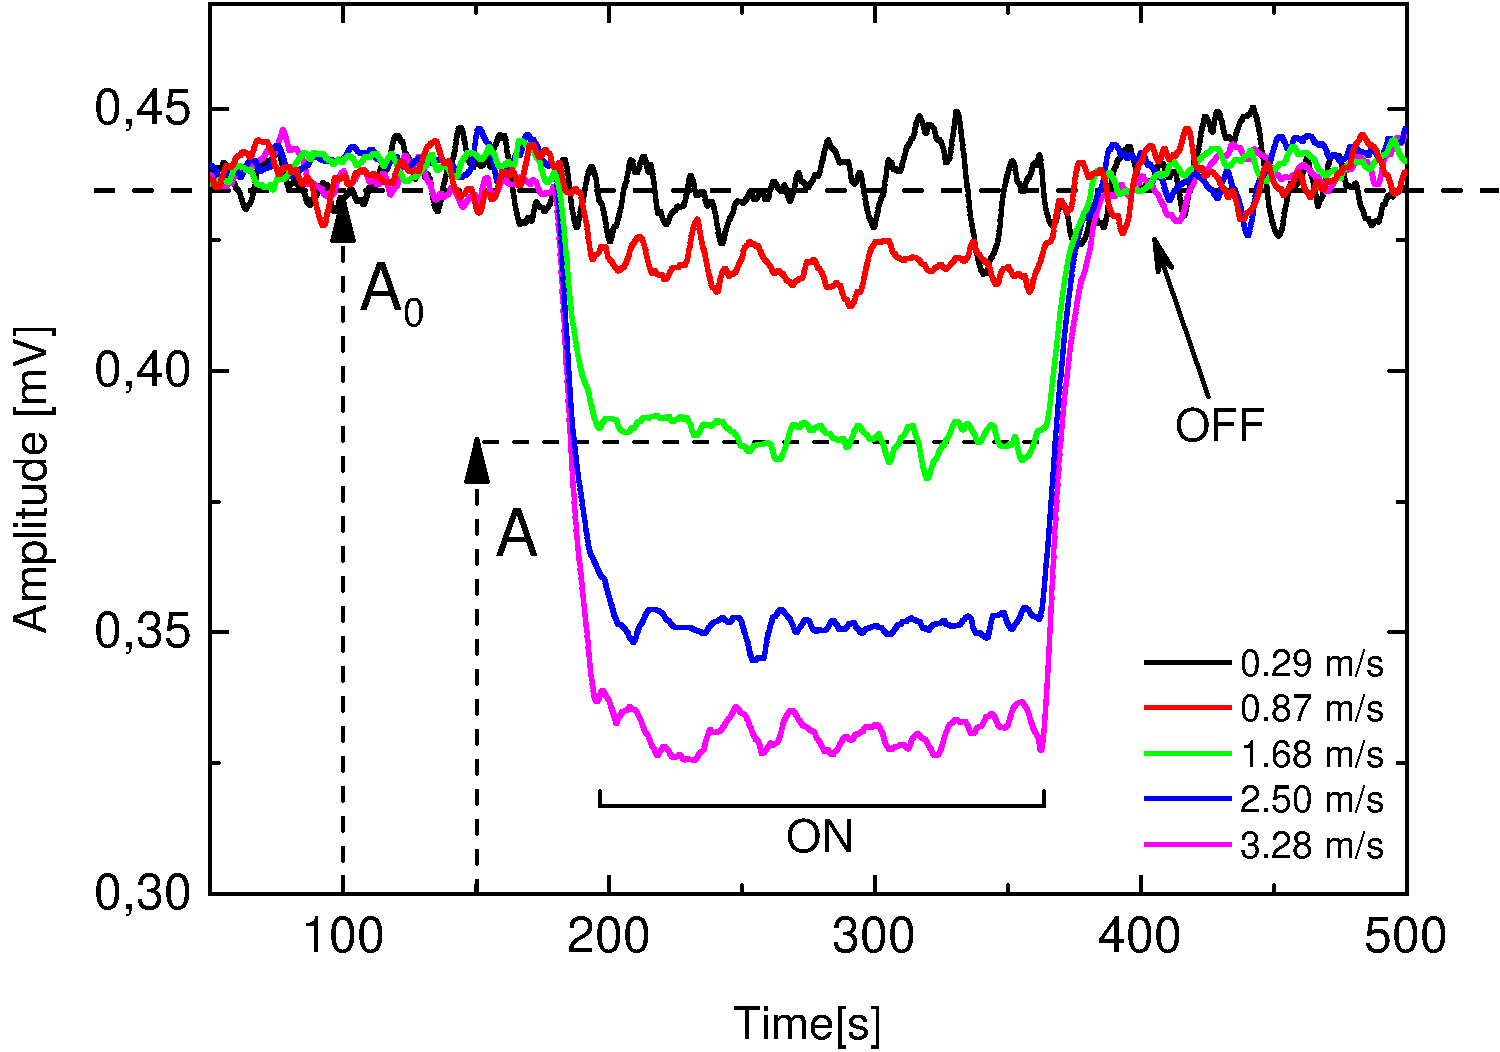
\includegraphics[width=0.75\textwidth]{graphs/Attenuation.pdf}
\caption{An example of second sound attenuation due to the presence of quantized vortices, produced by an oscillating tuning fork at various velocities. "ON" and "OFF" labels describe the state of the tuning fork. The time on the x-axis is measured from the beginning  of each particular run. Values shown in this graph are taken at the temperature $ T=1.95\unit{K} $. The measurement at the velocity of $0.29\unit{m/s}$ corresponds to a vortex line density $L_0 = 3 \times 10^6 \unit{m}^{-2}$ and is taken as an estimate of the sensitivity threshold of our measurement technique.}
\end{figure}

The five aforementioned steps were repeated for several values of voltage applied across the tuning fork, for both fundamental and overtone mode at all six temperatures (all of the above except $ 1.65 \unit{K}$). We have always proceeded from low values of driving voltage to higher ones gradually, so that it is clear, at which point any measurable amount of quantum vortices appears.

By collecting datasets of $ A $, $ A_0 $ and $ \Delta f_0 $ we could estimate the vortex line density $ L $:

\begin{equation}
L = \frac{6\pi \Delta f_0}{B\kappa}\bigg( \frac{A_0}{A} - 1 \bigg)\,,
\label{eq}
\end{equation}

and the fork tip velocity $ v=I/a $, where $ I $ is current response and $ a $ the fork constant. The resulting plot ({\sffamily\textbf{Figure 3.3}}) is shown below.

We should point out that the results for $ L $ as derived in {\sffamily\textbf{Section 1.6}} are valid only for homogeneously and isotropically distributed vortices. The amount of quantized vortices is expected to be higher near the fork than further away from it. Since we utilized the $ 1^{\ind{st}} $ second sound resonant mode, we have, in fact, measured the $ 1^{\ind{st}} $ Fourier component of the vortex line density spatial distribution\cite{Emilfluids}. This is sufficient for the purposes of (roughly) estimating the quantities of quantized vortices produced, but the true values of $ L $ near the tuning fork may differ by some factor and could be obtained only by measurements using several additional second sound resonant modes.

\begin{figure}[h!]
	\centering
	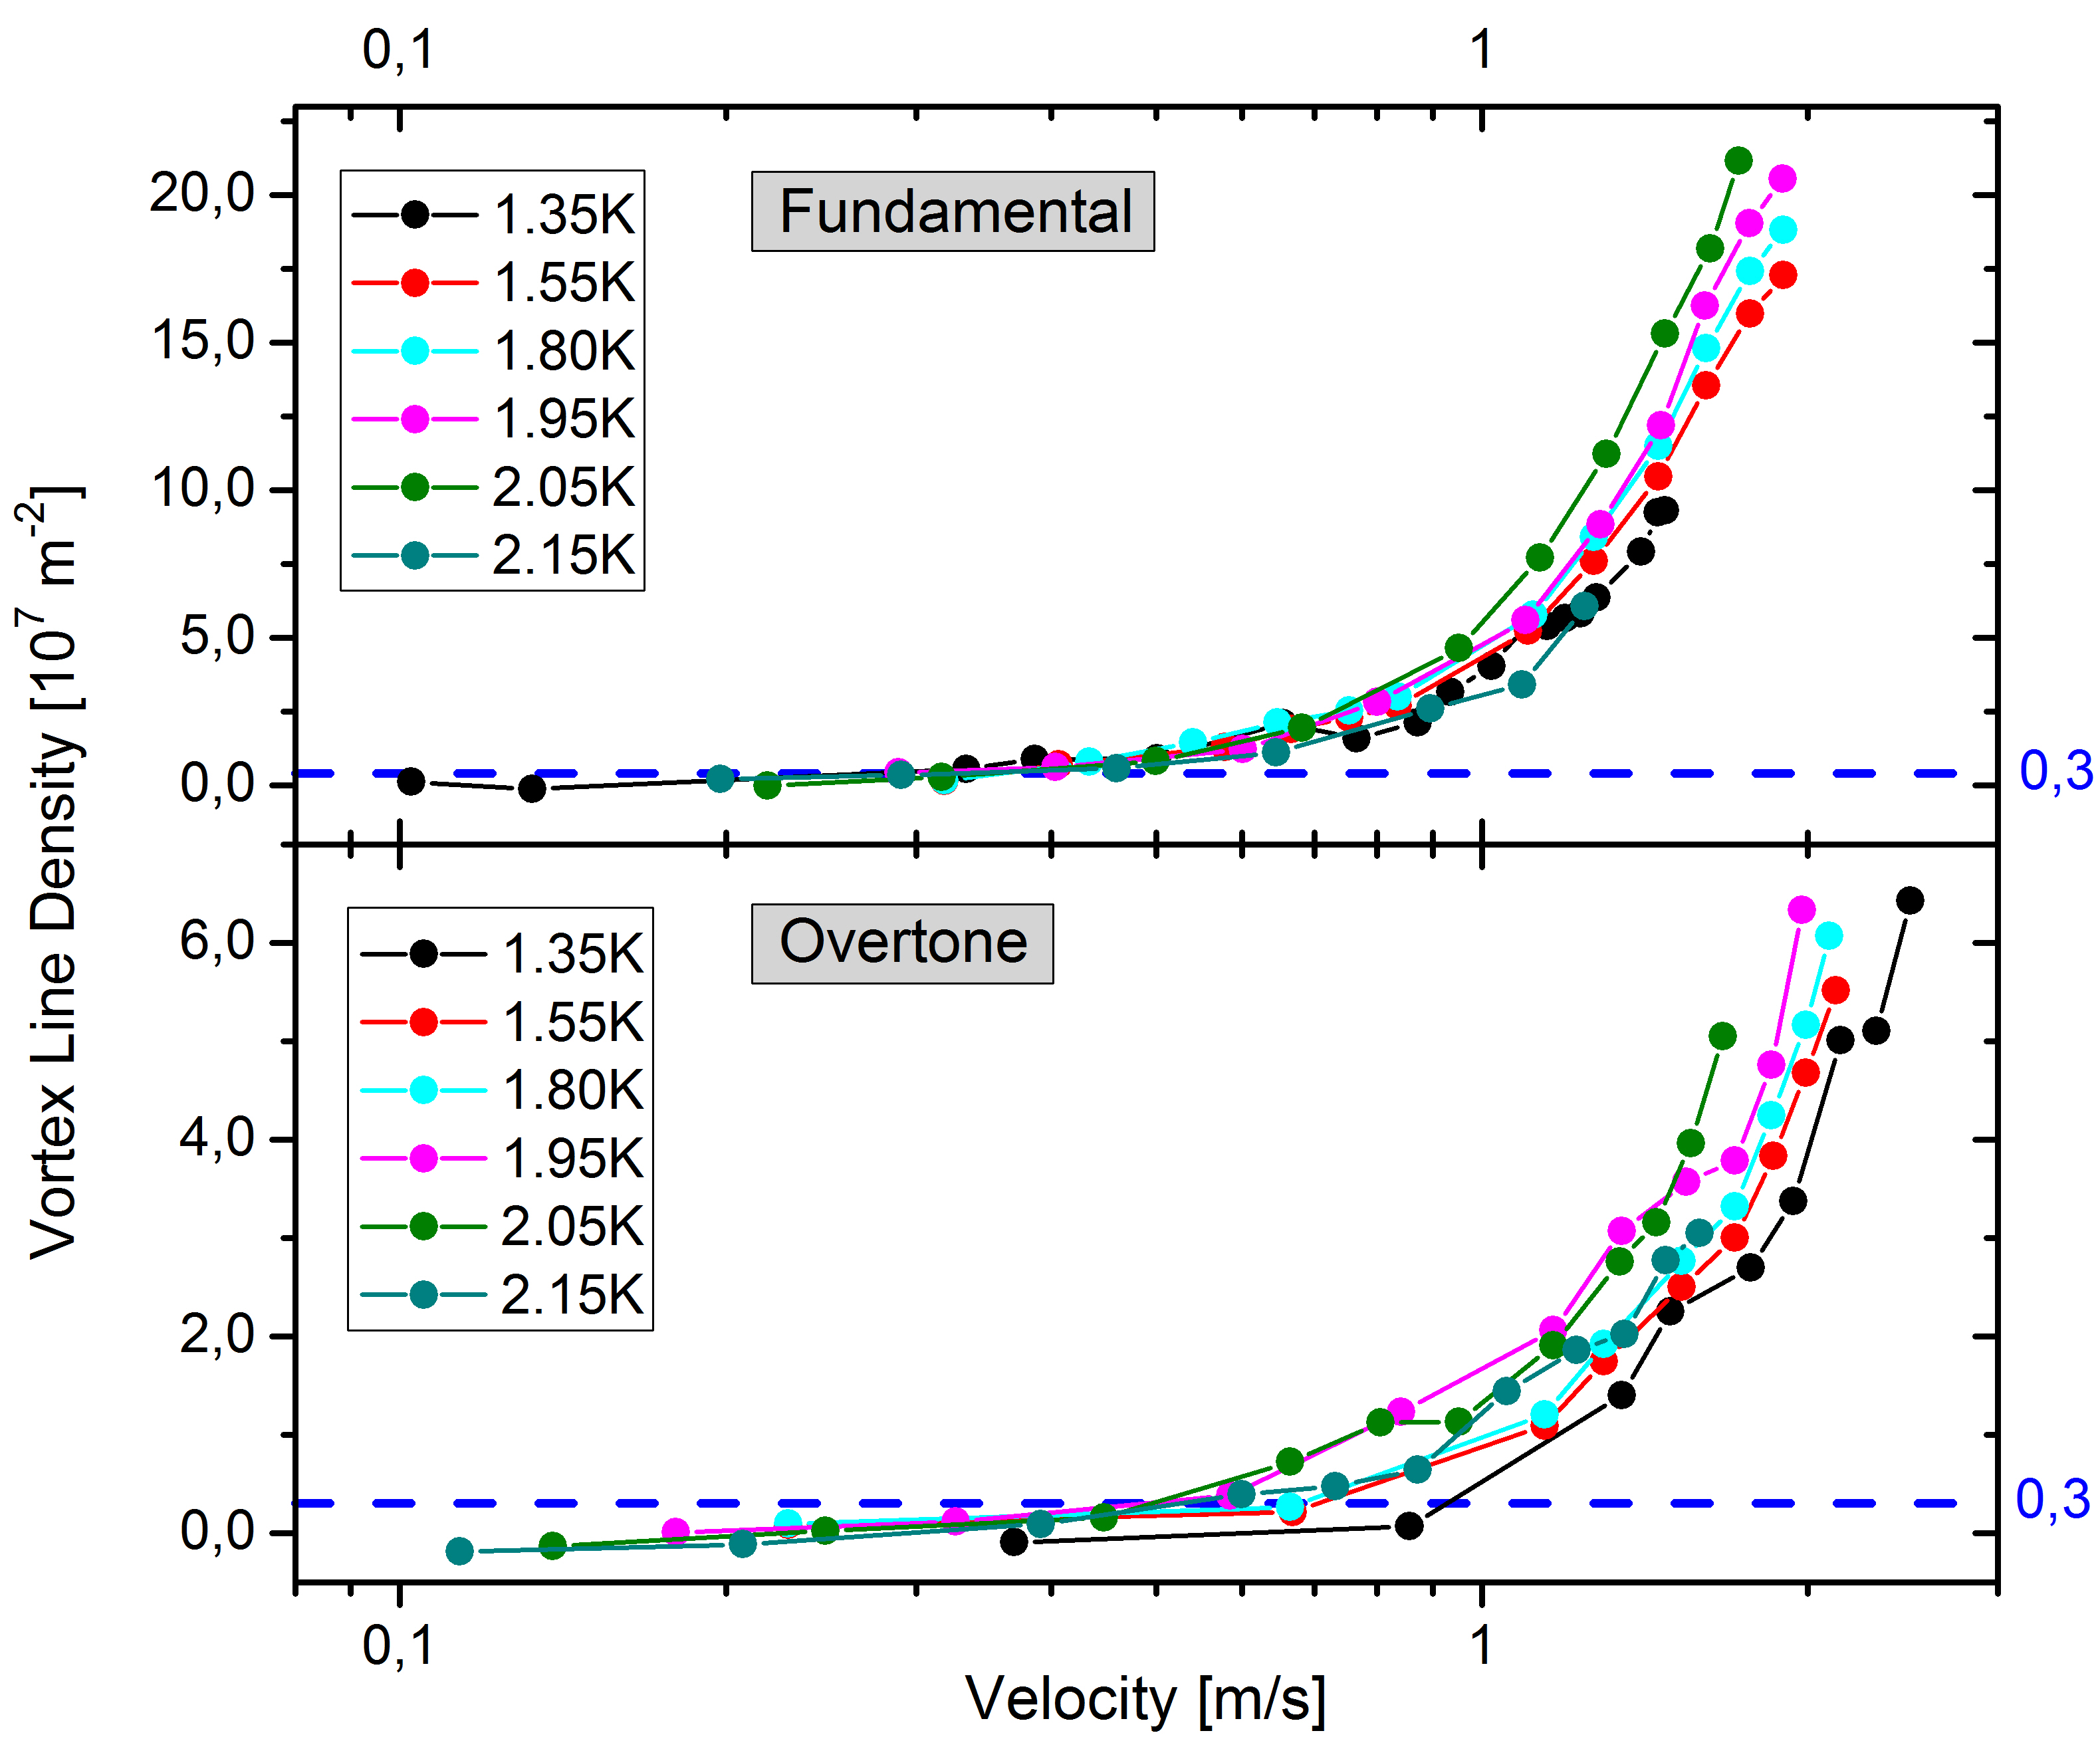
\includegraphics[width=1\textwidth]{graphs/Merged_L_v(abs)}
	\caption{Vortex line density $ L $ against the (logarithmically scaled) peak velocity of the tuning fork $ v $. The \textit{blue dotted line} marks the threshold level $ L_0 \approx 3\cdot 10^6 \unit{m}^{-2} $ introduced in {\sffamily\textbf{Figure 3.2}}, above which the measured vortex line density can be regarded as reliable.}
\end{figure}


Nevertheless, from {\sffamily\textbf{Figure 3.3}} we observe that no significant amounts of vortex lines are produced before a certain critical velocity is exceeded. Furthermore, we find that the amount of quantized vortices produced is temperature-independent and scales only with the velocity of the tuning fork.

Plotting $ L $ on a logarithmic scale we observe (see {\sffamily\textbf{Figure 3.4}}) that the critical velocities, above which the quantum vortices are produced in much larger amounts, are also independent of temperature.
Bearing in mind the sensitivity threshold, we estimate these critical velocities for the fundamental and overtone modes to be $ v_{\ind{c}}^{\ind f} = 0.3 \pm 0.1 \unit{m/s}$, and $ v_{\ind{c}}^{\ind o} = 0.7 \pm 0.2 \unit{m/s} $, respectively. Moreover, as noticed in {\sffamily\textbf{Section 1.10}}, the critical velocity should scale with frequency as $ \propto \sqrt{\kappa\omega} $. From our results we get $ v_{\ind{c}}^{\ind f}/ v_{\ind{c}}^{\ind o} \cdot \sqrt{f_0^{\ind{o}}/f_0^{\ind{f}}} \doteq 1.06 $, which is consistent with the given scaling.

\newpage

\begin{figure}[h!]
	\centering
	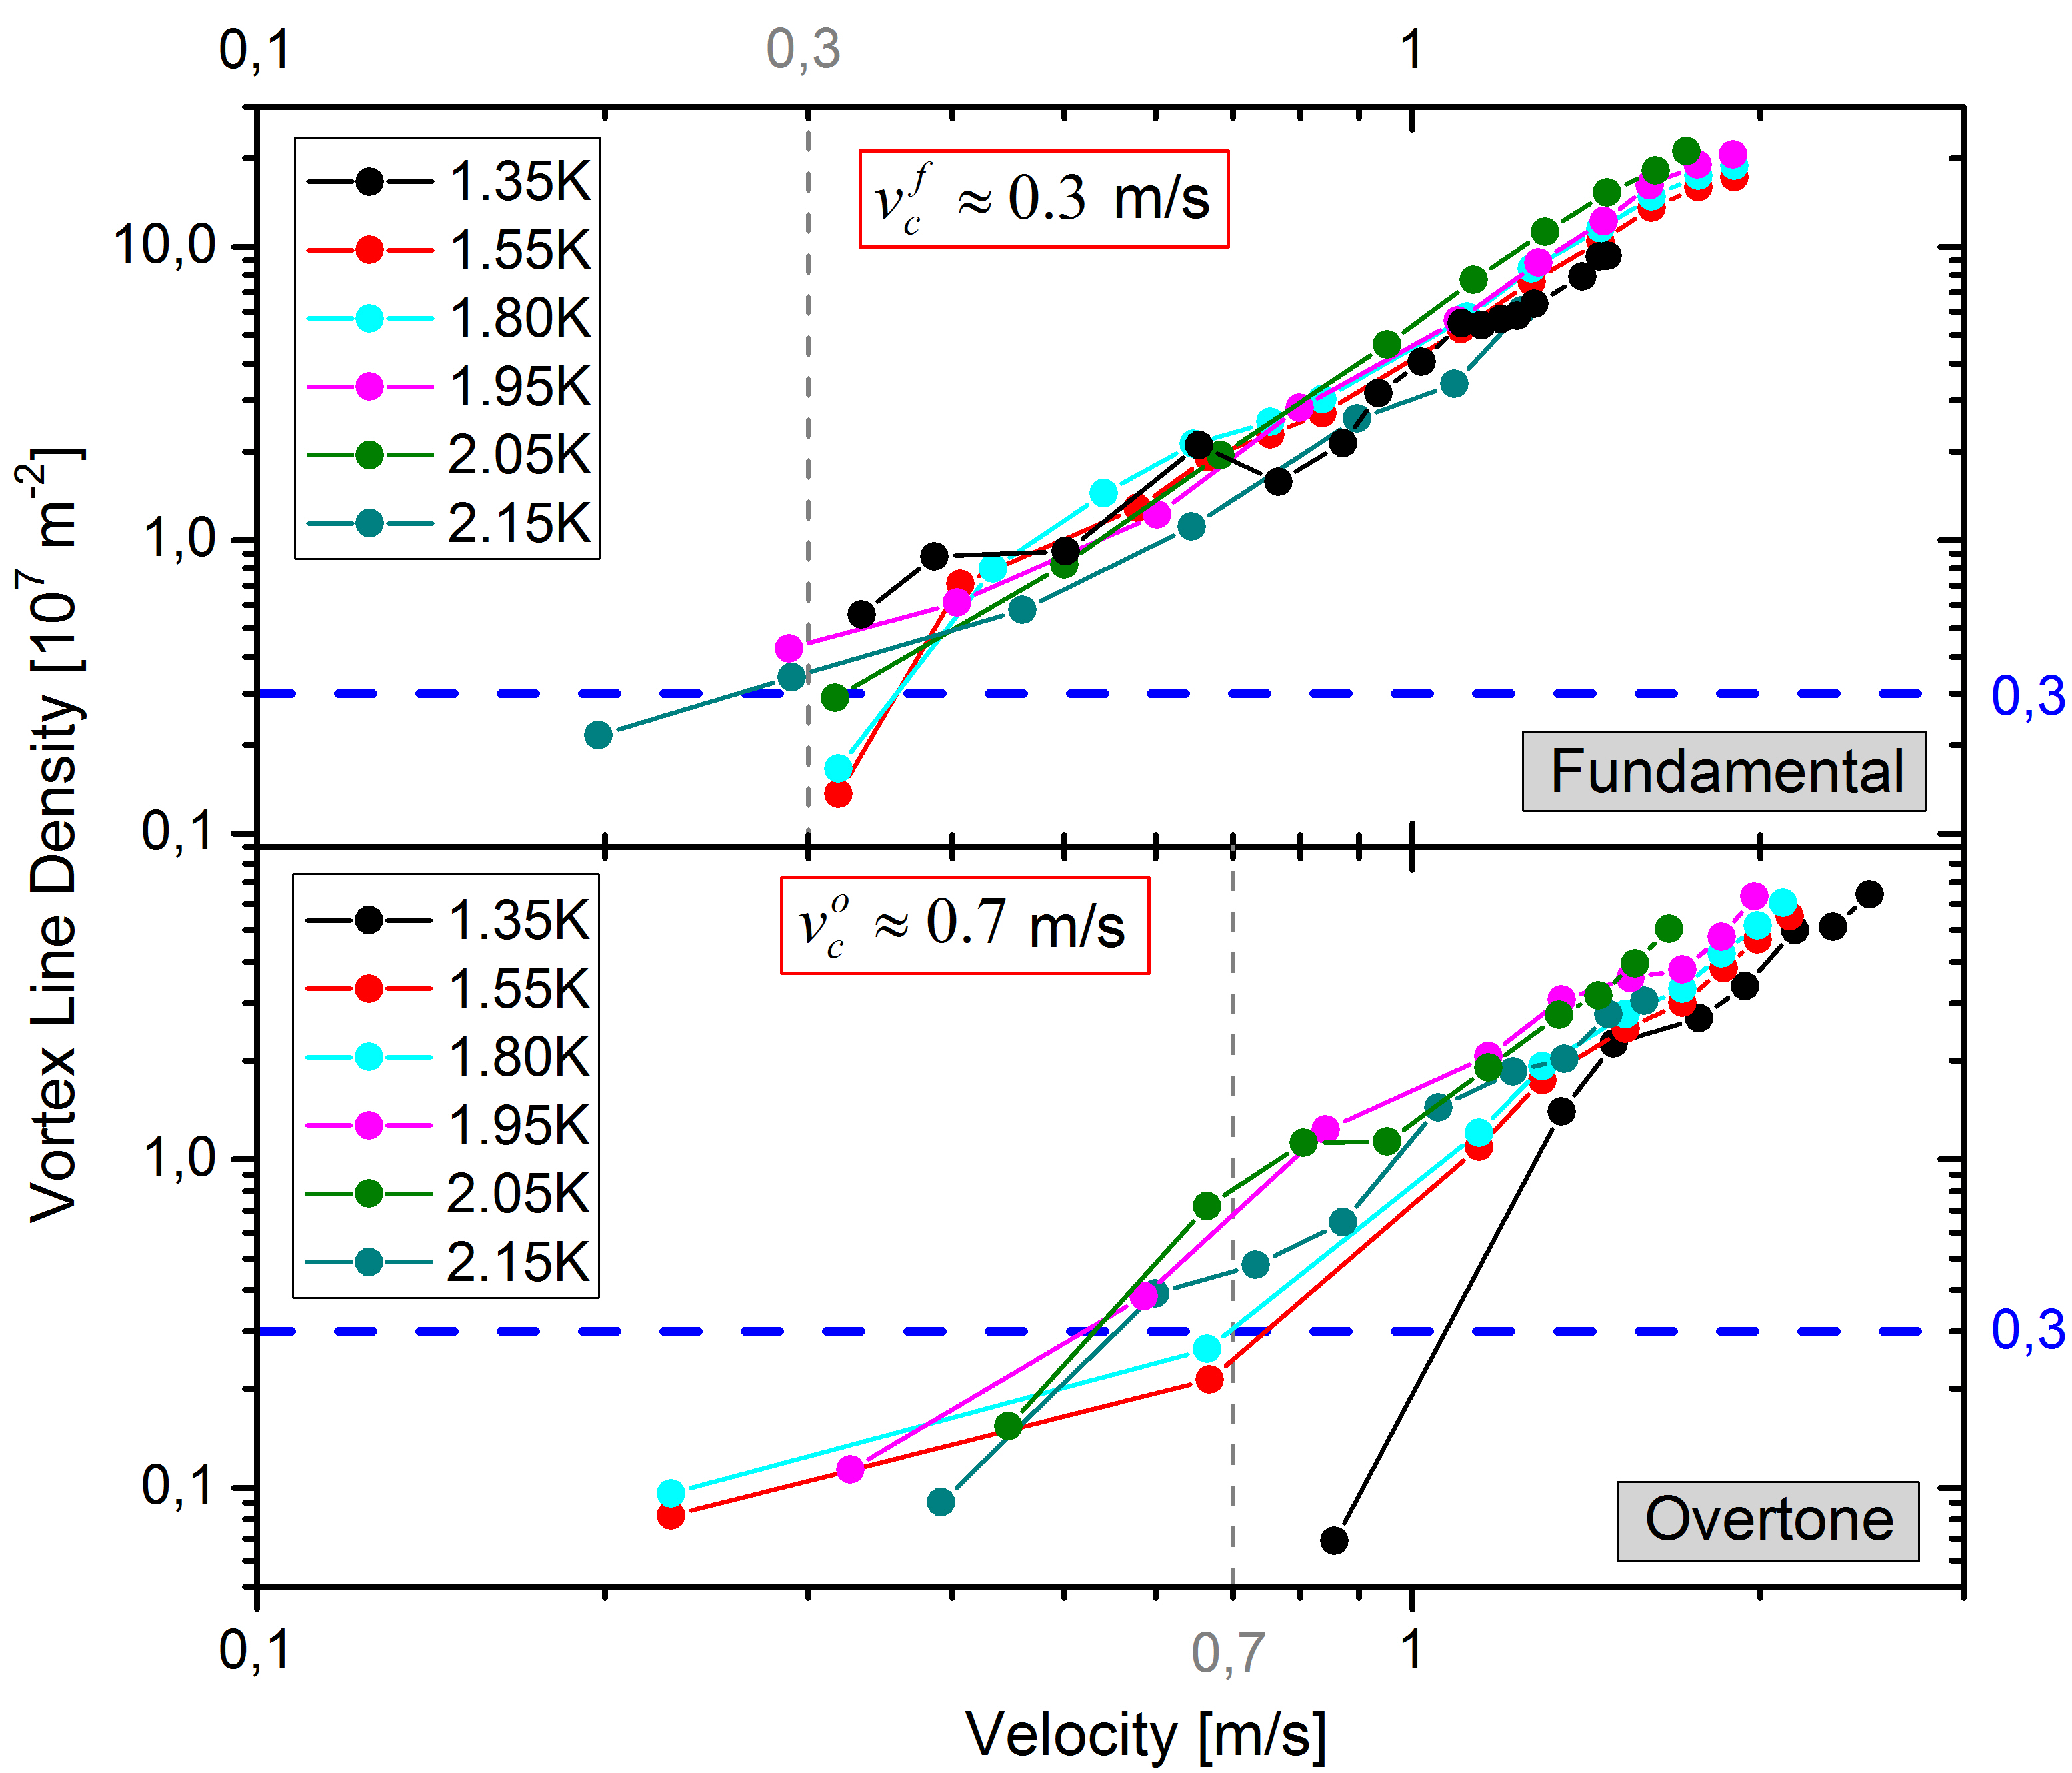
\includegraphics[width=1\textwidth]{graphs/Merged_L_v(log)}
	\caption{Log-log graph of the vortex line density $ L $ against the peak velocity of the tuning fork (the same data as in {\sffamily\textbf{Figure 3.3}}). This graph better illustrates the position of threshold $ L_0 \approx 3\cdot 10^6 \unit{m}^{-2} $ (\textit{blue dashed lines}) and the temperature-independent critical velocities (\textit{grey dashed lines}). The tuning fork peak velocity is determined with an uncertainty of about $ 10\%$ that arises from the electrical calibration procedure\cite{opticalfork}. The vortex line density is affected by a systematic error that is mainly due to the assumption of a homogeneous isotropic tangle in deriving (\ref{eq}) that obviously does not correspond to the vortex tangle produced in the vicinity of the tuning fork.}
\end{figure}


Increasing the sensitivity of the second sound measurement (and thus lowering the threshold level) would allow determining the critical velocities with better accuracy and reduce the scatter in the observed data. Although the design of the second sound resonator and sensors is far from perfect, the current sensitivity is sufficient for a qualitative discussion of the relationship between the obtained vortex line densities and the drag forces acting on the tuning fork.


\newpage

\section{Drag Force Measurements}

All of drag force measurements presented in this Section were done solely with the tuning fork; second sound was not used during the measurement. We have operated the tuning fork in full frequency sweeps, with gradually increasing/decreasing driving voltages. Each of the datapoints in the following graphs is thus obtained from a full frequency sweep of tuning fork around its fundamental or overtone resonance frequency with a given applied voltage $ U_0 $. From such a sweep, the current response $ I $ was measured and for each pair $ \big[U_0,I\big] $ we found the corresponding values of peak applied force and peak velocity $ \big[F,v\big] $ using the calibration formulae from \cite{forks}: $ F = a U_0/2 $, $ v = I/a $.

\begin{figure}[h!]
	\centering
	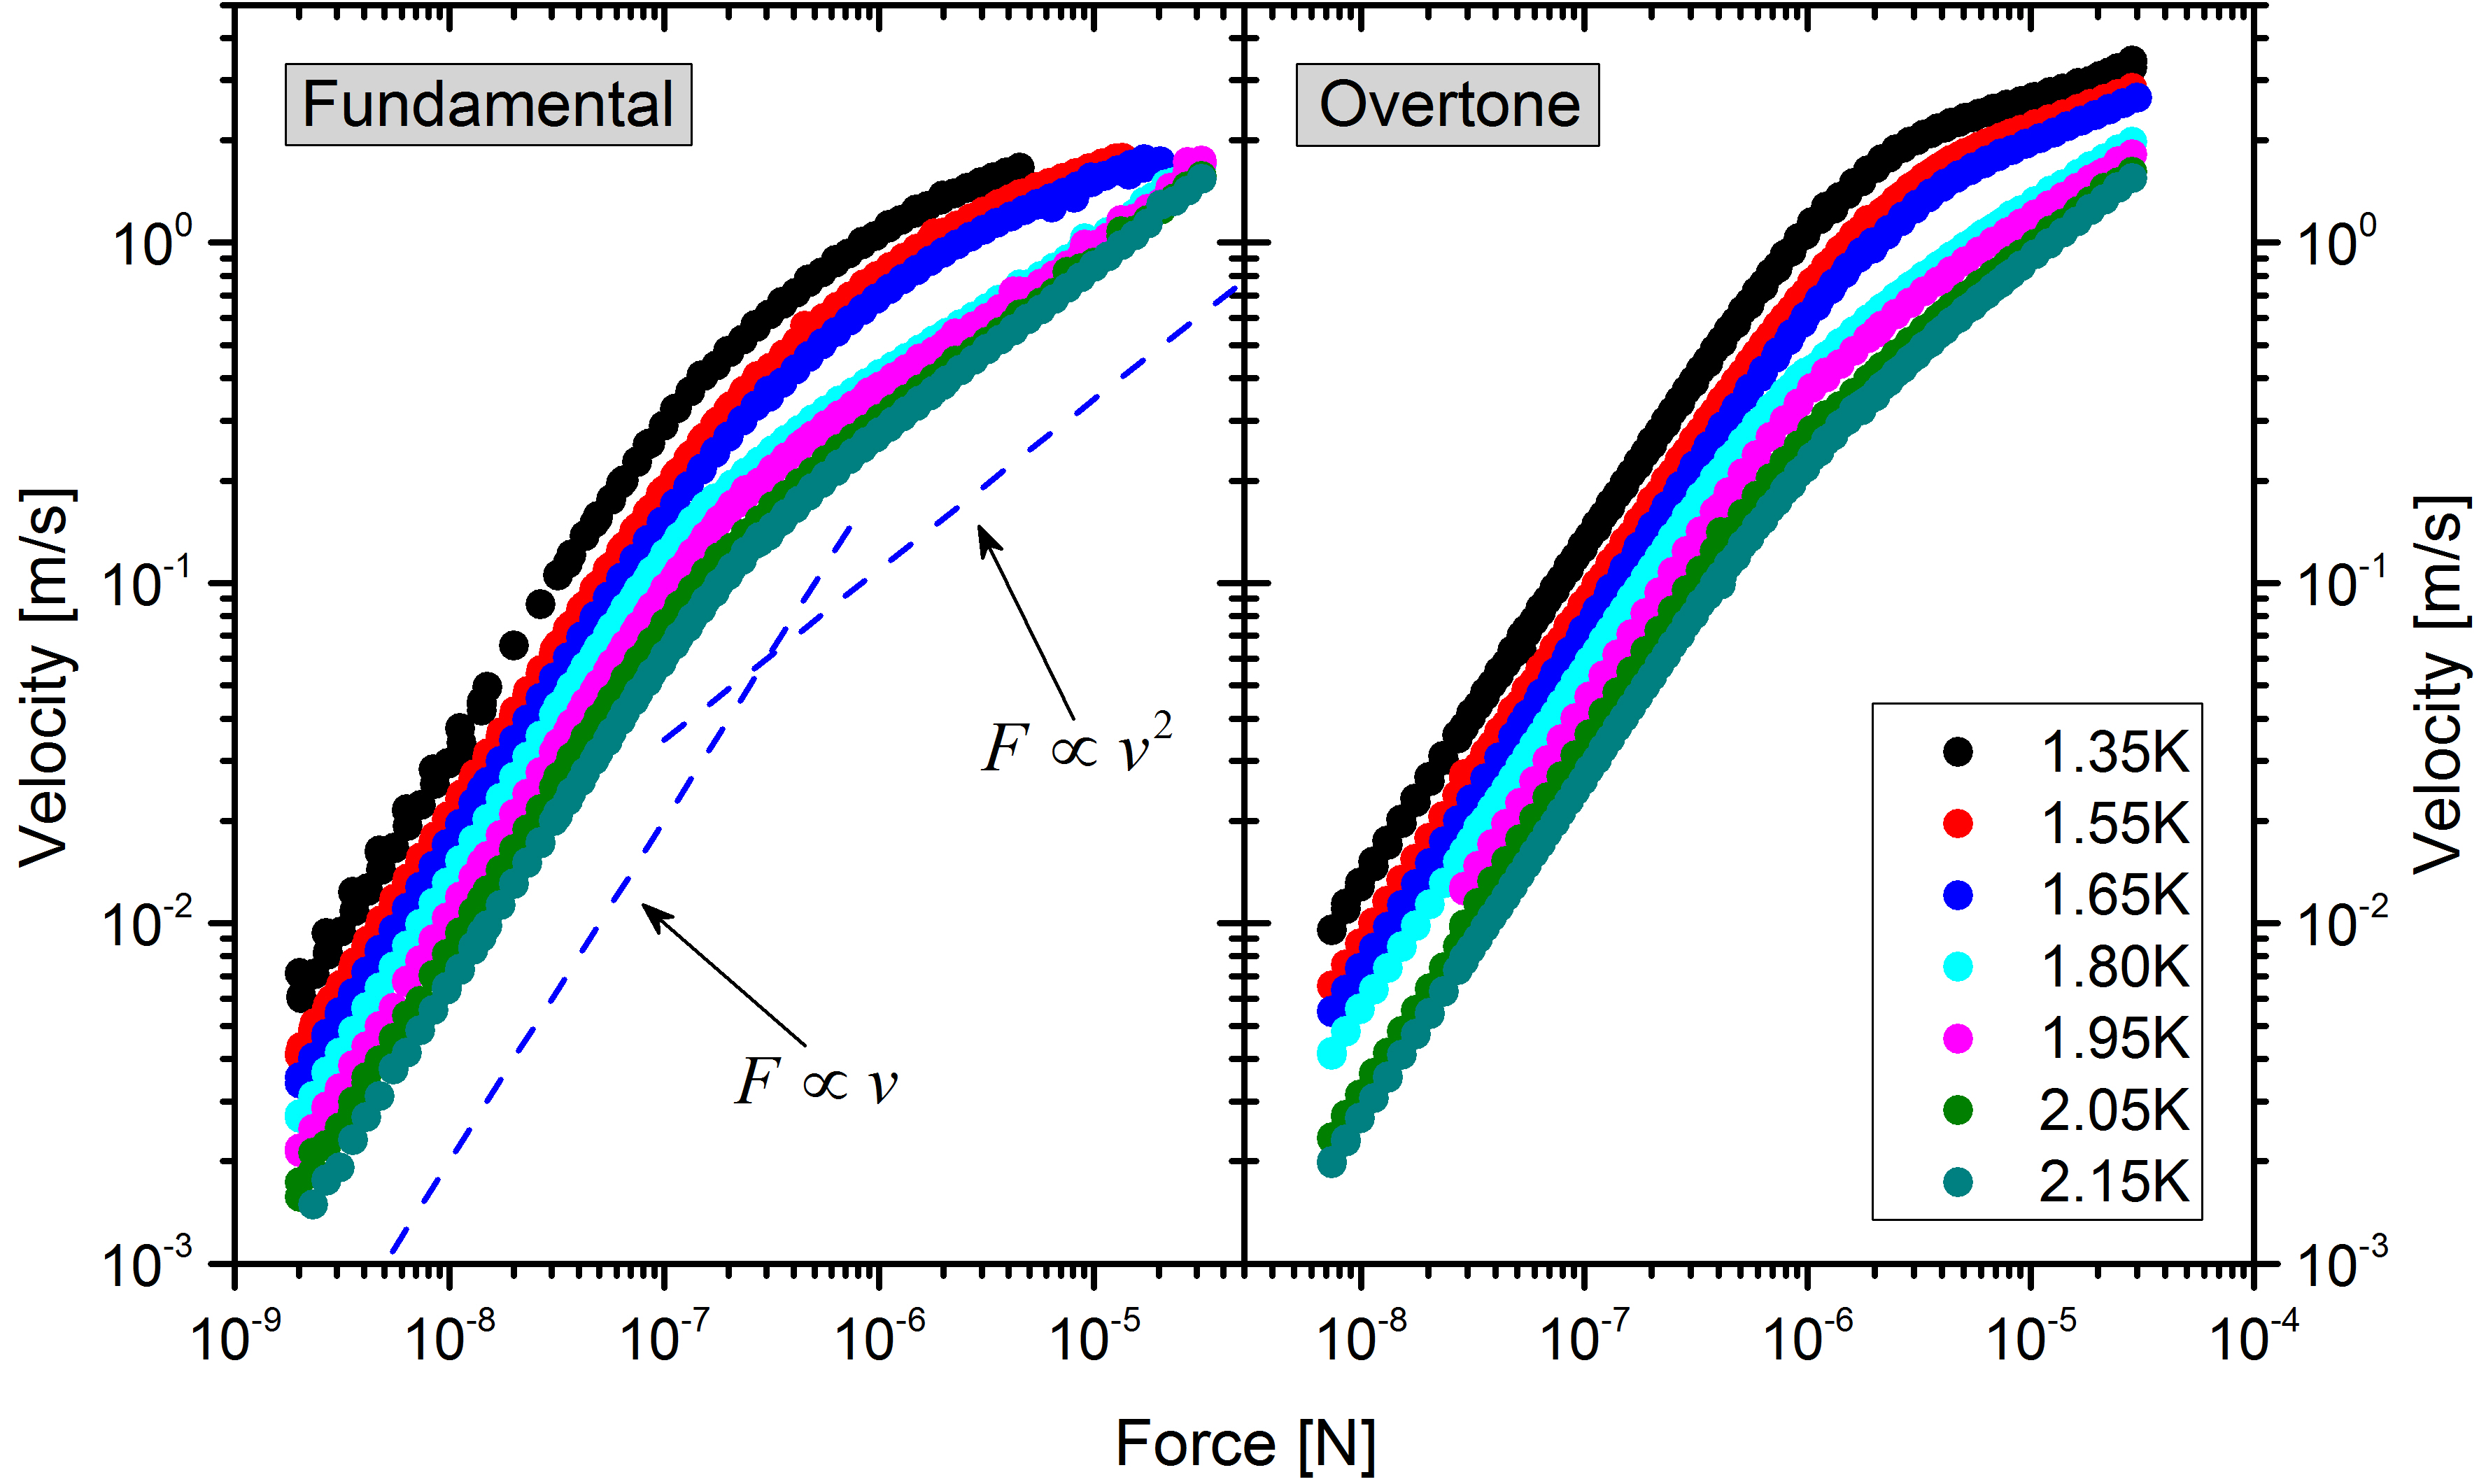
\includegraphics[width=1\textwidth]{graphs/Merged_v_F}
	\caption{Force-Velocity characteristics for the fundamental and overtone modes of our tuning fork at seven different temperatures spanning the two-fluid regime. Apparently, a transition from linear to non-linear drag force occurs at high enough velocities. The \textit{blue dotted lines} sketch the approximate theoretical dependencies for laminar and classical turbulent flow.}
\end{figure}

In {\sffamily\textbf{Figure 3.5}} a transition from linear to non-linear drag is clearly observed. In classical fluid mechanics, the onset of force non-linearity is interpreted as a formation of a wake past the bluff body that encompasses vortical motion of the fluid and may eventually lead to the generation of turbulence. Our case is more complicated since we deal with two (possibly interacting) fluids and hence with two mutually-dependent types of turbulent motion.

It is also apparent that the linear drag force strongly depends on temperature, which reflects the fact that only the normal component contributes to the drag force in laminar flow. At the same time, the superfluid component exhibits purely potential flow, as an ideal fluid might, which results in a zero net contribution to the drag force as per d'Alembert's paradox \cite{landau}. To discuss the scaling properties in greater detail, it is, however, necessary to convert the force and velocity into relevant dimensionless quantities, such as the drag coefficient $ C_{D} = 2F/S\rho v^2 $ and the oscillatory Reynolds number $ \text{Re}_{\delta} = v\rho\delta/\eta $, , where $ S $ stands for the cross-section area of fork perpendicular to the direction of oscillation and $ F $ for the measured drag force.


\begin{figure}[h!]
	\centering
	\vspace{-0.3cm}
	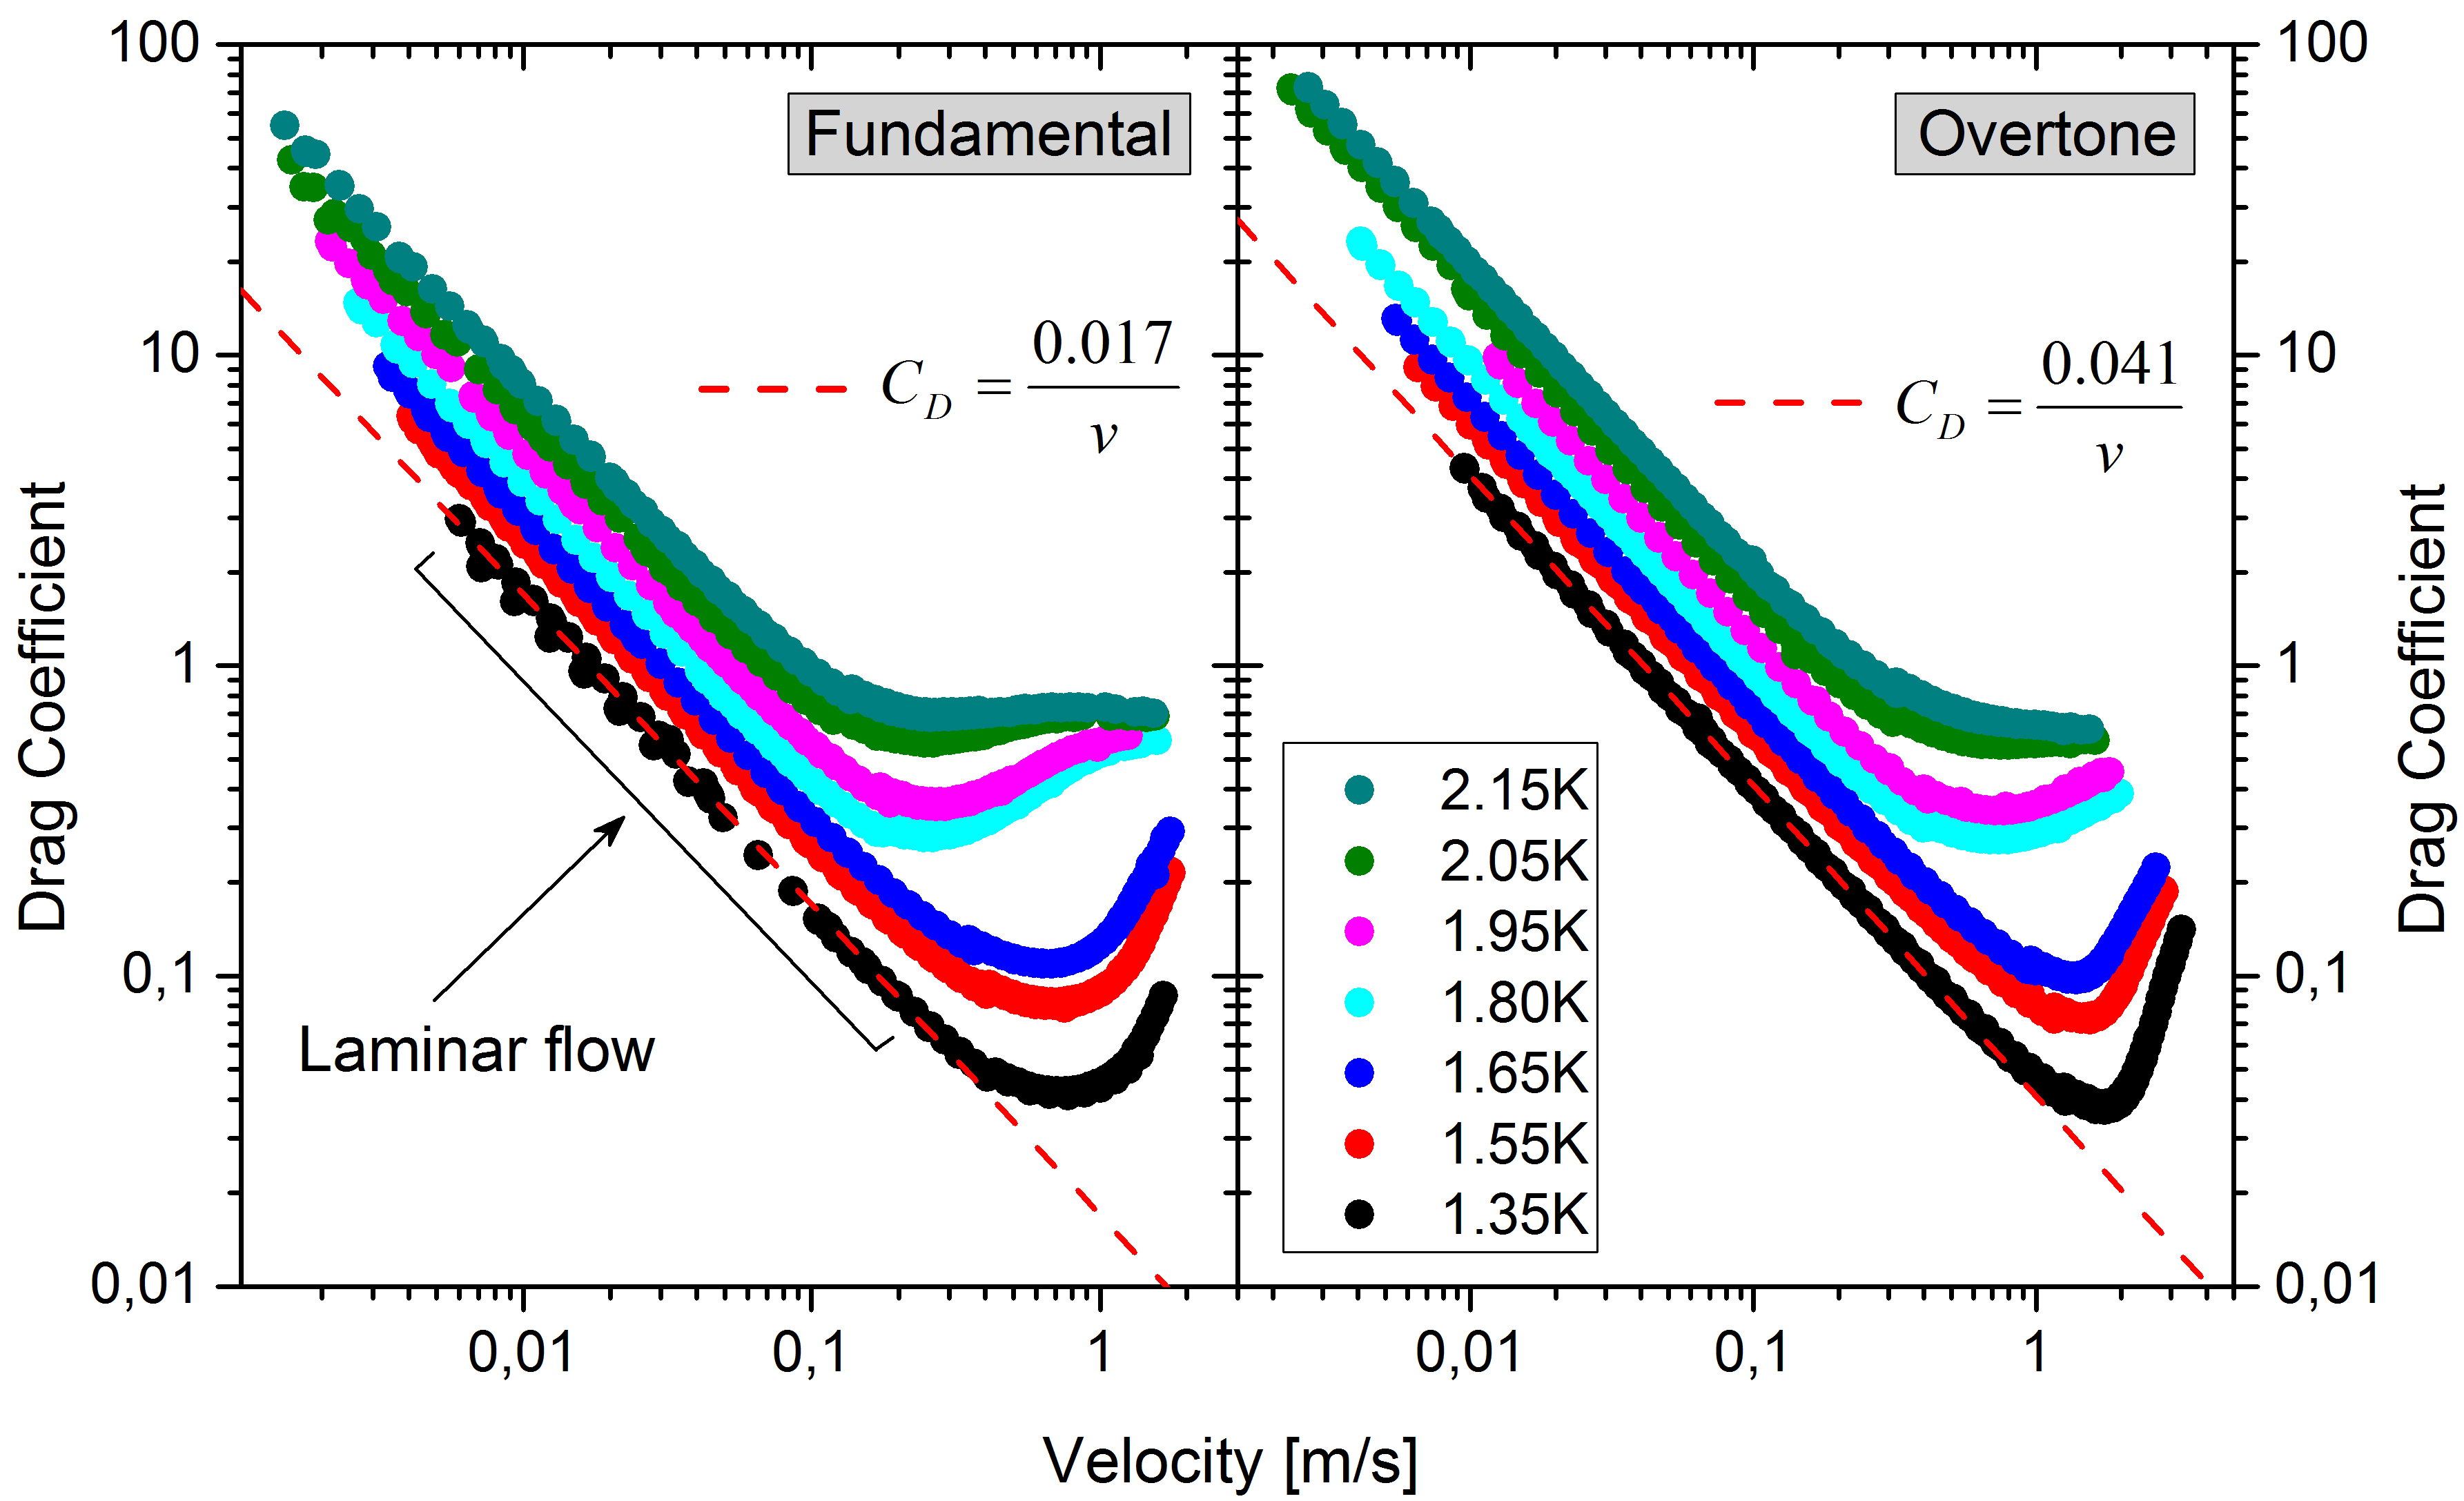
\includegraphics[width=1\textwidth]{graphs/Merged_C_v}
	\caption{Drag coefficients plotted against the peak velocity of the oscillating tuning fork. The \textit{red dotted lines} fit the laminar part of the dependences for the temperature $ 1.35\unit{K} $, with different values of the fitting parameter for the two tuning fork modes. }
\end{figure}

Looking at the graph in {\sffamily\textbf{Figure 3.6}} we can recognize ``two types'' of curves. Those for which the non-linearity seemingly appears at one certain velocity, and those for which the onset arises when exceeding different velocities. This can be regarded as the first sign that either quantum turbulence (QT) or classical turbulence (CT) may occur first under different conditions. Moreover, we note that the $ 2.15 \unit{K}$ curve seems to approach the dependence of the drag coefficient as we know it from classical fluids, with the limiting constant value not far below $ C_D = 1 $, which is expected for tuning forks in a classical fluid~\cite{PraguePRB}.

Within the two-fluid model, we distinguish between the drag coefficient and oscillatory Reynolds number for the whole fluid $ C_{D}$, $ \text{Re}_{\delta} $ and only for the normal component alone $ C_{D{\ind n}} = 2F/S\rho_{\ind n}v^2 = C_D \rho/\rho_{\ind n} $, $ \text{Re}_{\delta_{\ind n}} = v\rho_{\ind n}\delta_{\ind n}/\eta_{\ind n} $. For each temperature, the values for the density of normal component $ \rho_{\ind n} $ and dynamical viscosity were taken from \cite{donnelly}.

The resulting graph ({\sffamily\textbf{Figure 3.7}}) showcases three interesting and important facts. First, within the laminar range, all curves collapse to a single dependence, confirming the validity of the scaling proposed in {\sffamily\textbf{Sections 3.3, 3.4}} and establishing the oscillatory Reynolds number as a suitable dimensionless parameter. Second, for both modes, the laminar part could be fit by the exact same straight line. This represents the fact that the drag force scaling in the high-frequency regime is, with all likelihood, independent on the velocity profile along the prong and holds even for frequencies differing by a factor of $40\,000/6380\approx 6.27 $. Finally, the critical Reynolds number for generating classical turbulence within both fork modes (the $ 2.15\unit{K} $ curve best shows) has been estimated as $ \text{Re}_{\delta_{\ind n}c}=7\pm 2 $.




\begin{figure}[h!]
	\centering
	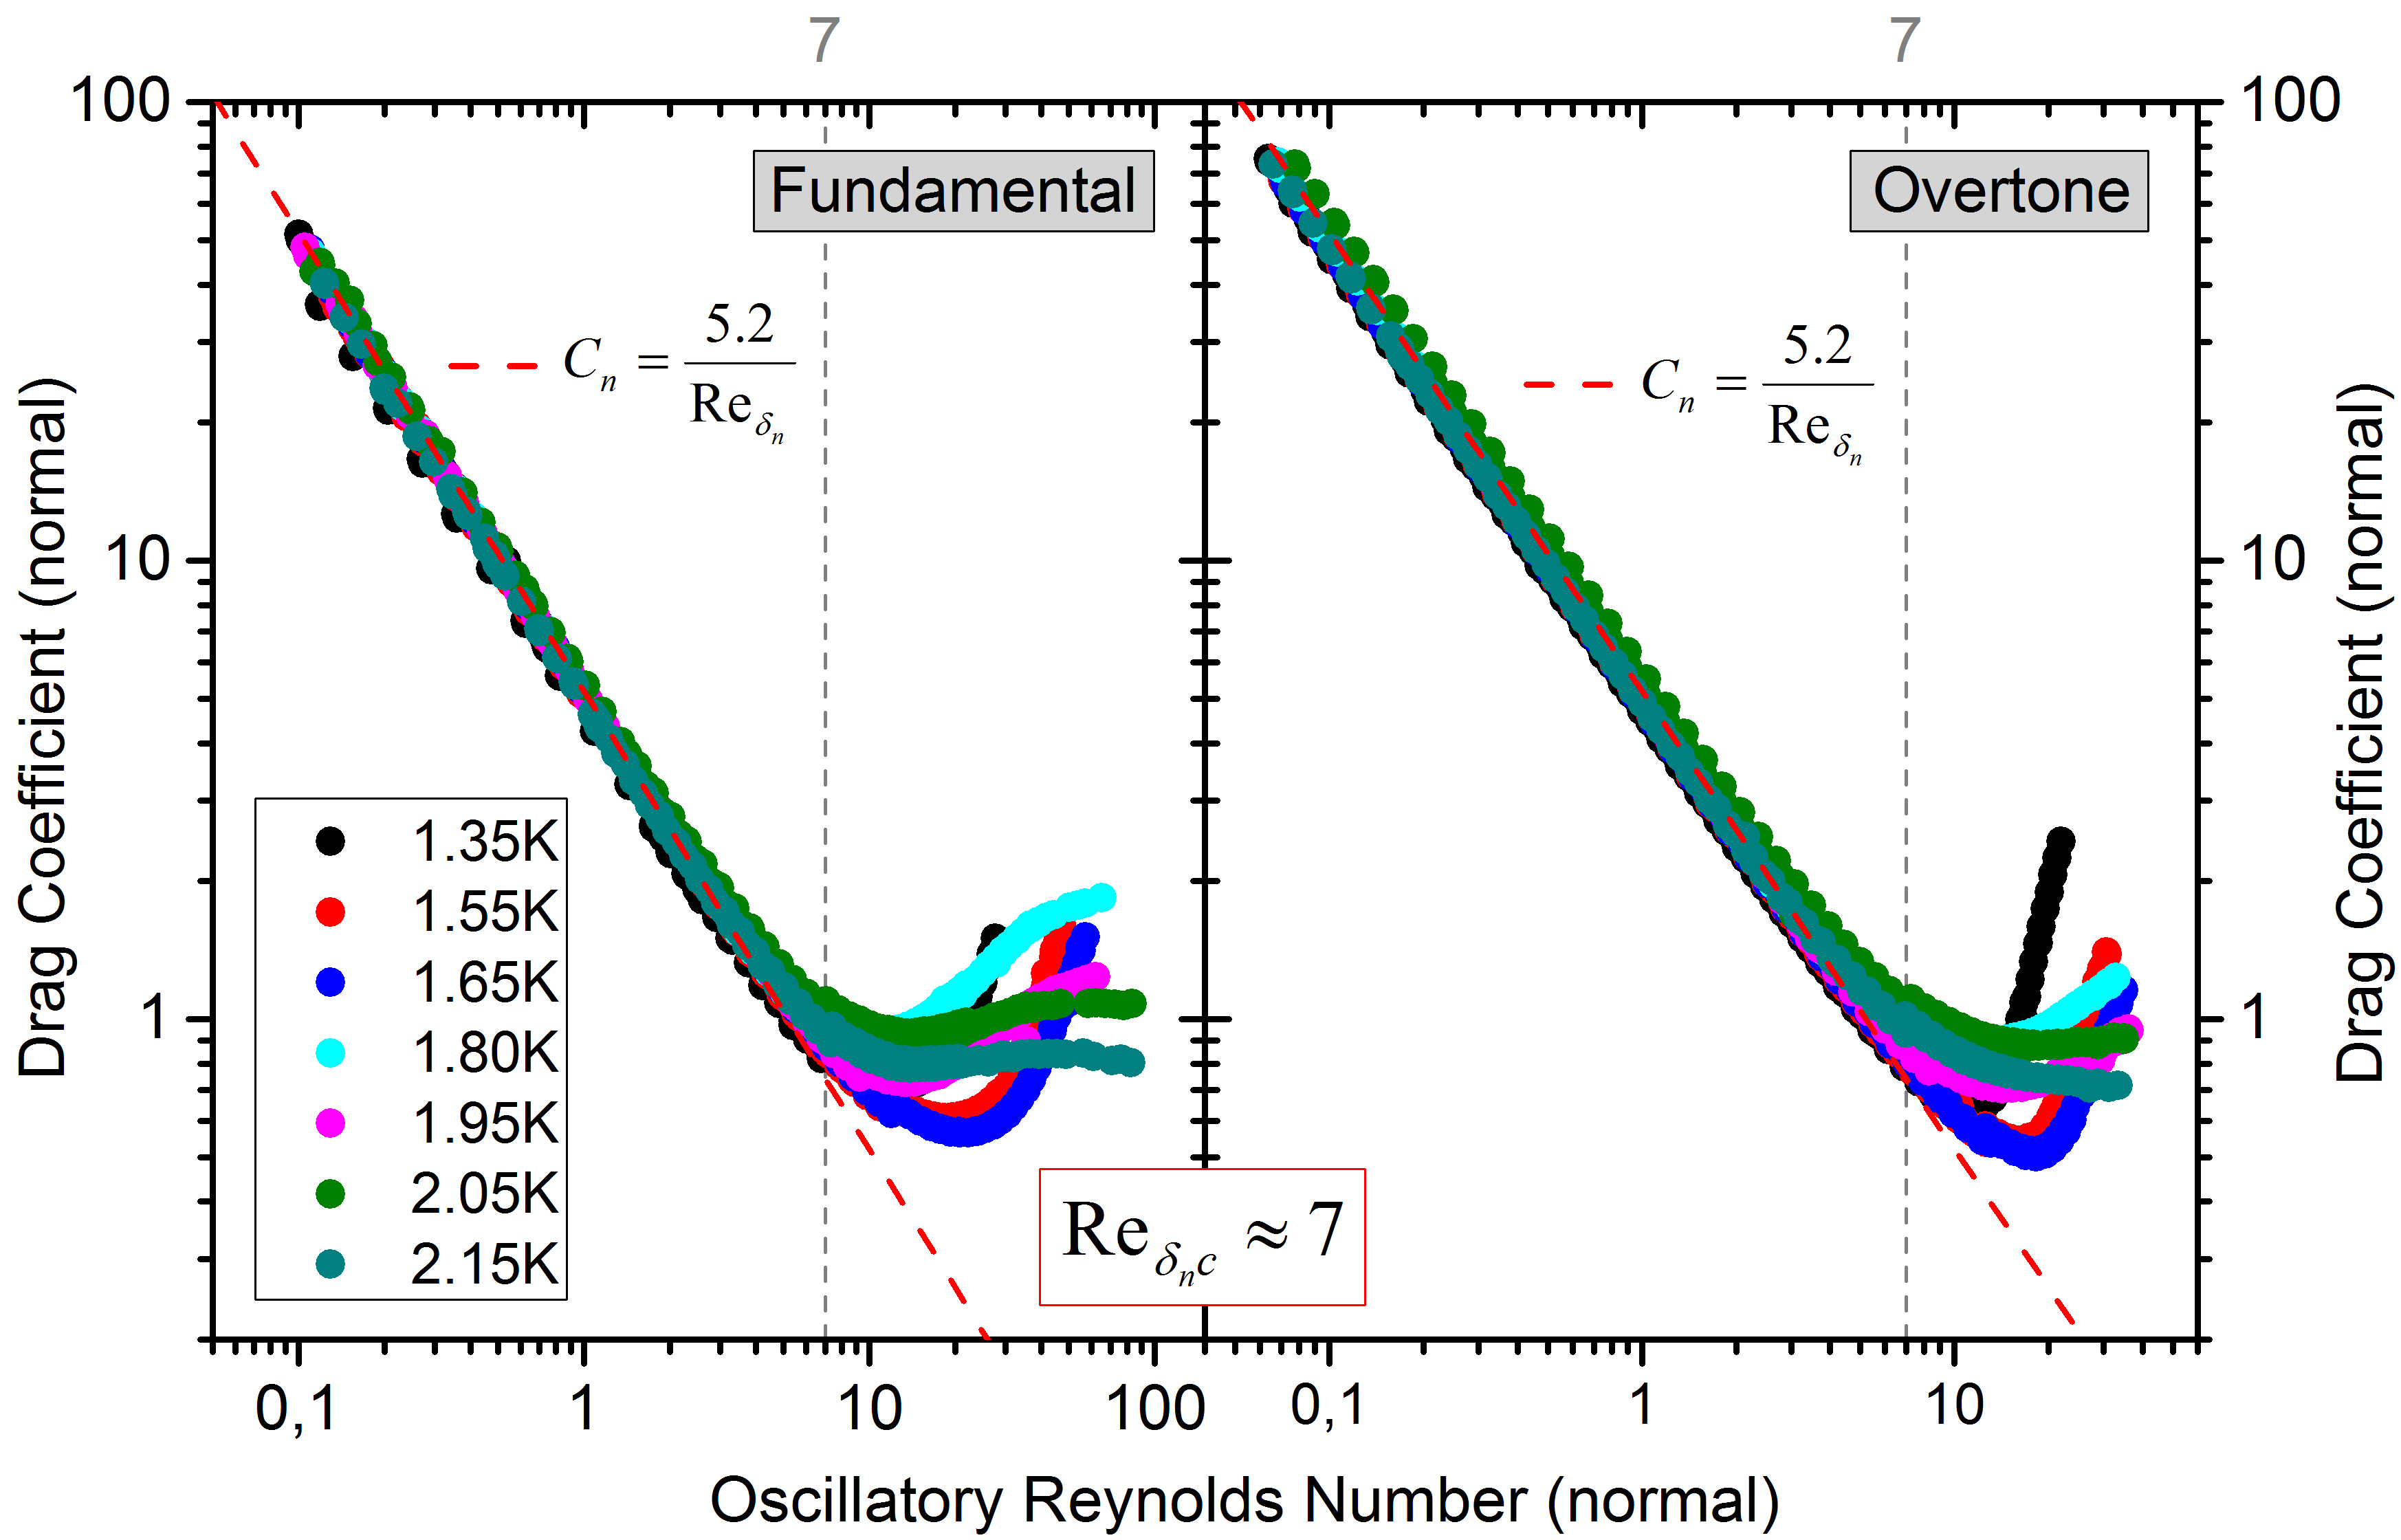
\includegraphics[width=1\textwidth]{graphs/Merged_Cn_Ren}
	\caption{Drag coefficient plotted against the oscillatory Reynolds number, both evaluated for the normal component alone. Statistically, the onset of non-linear drag occurs for all temperature curves within the interval $ \text{Re}_{\delta_{\ind n}}^{\ind{crit}}=7\pm 2 $. The presented data are, however, affected by the observed unsystematic behaviour of the tuning forks with regard to the onset of non-linear drag, as discussed in the accompanying text. The \textit{red dotted line} shows the fit of the laminar regime, which is exactly the same for both modes.}
\end{figure}

At this point, we have to remind the reader that during the actual experiment, we have observed unsystematic behaviour of the tuning forks and therefore the data shown here is very likely affected by this issue. In drag force measurements, this manifested in such a manner that the onset of non-linear drag occurred at different values of $ \text{Re}_{\delta_{\ind n}} $ when the same temperature was studied at different points during the entire experiment. Therefore, the estimated critical value of $ \text{Re}_{\delta_{\ind n}c}=7\pm 2 $ ought to be taken with some reservations, as it corresponds only to a subset of the acquired data (the four higher temperatures), for which we have reasonable grounds to claim that no significant change of the tuning fork behaviour occurred in between the measurements. Nevertheless, the actual critical value (incorrect as it may be) has little bearing on the interpretation presented below, and we choose to use this particular value as it still describes the majority of the data with a good degree of accuracy.

\section{Correlation of Results}


In the following, we connect the results of vortex line density measurement and the non-linear behaviour of drag coefficient. We will be able to distinguish between quantum turbulence (QT), caused by the presence of quantized vortices and classical-like turbulence (CT) of the normal component. Within this Section, we work only with the fundamental mode.


\begin{figure}[h!]
	\centering
	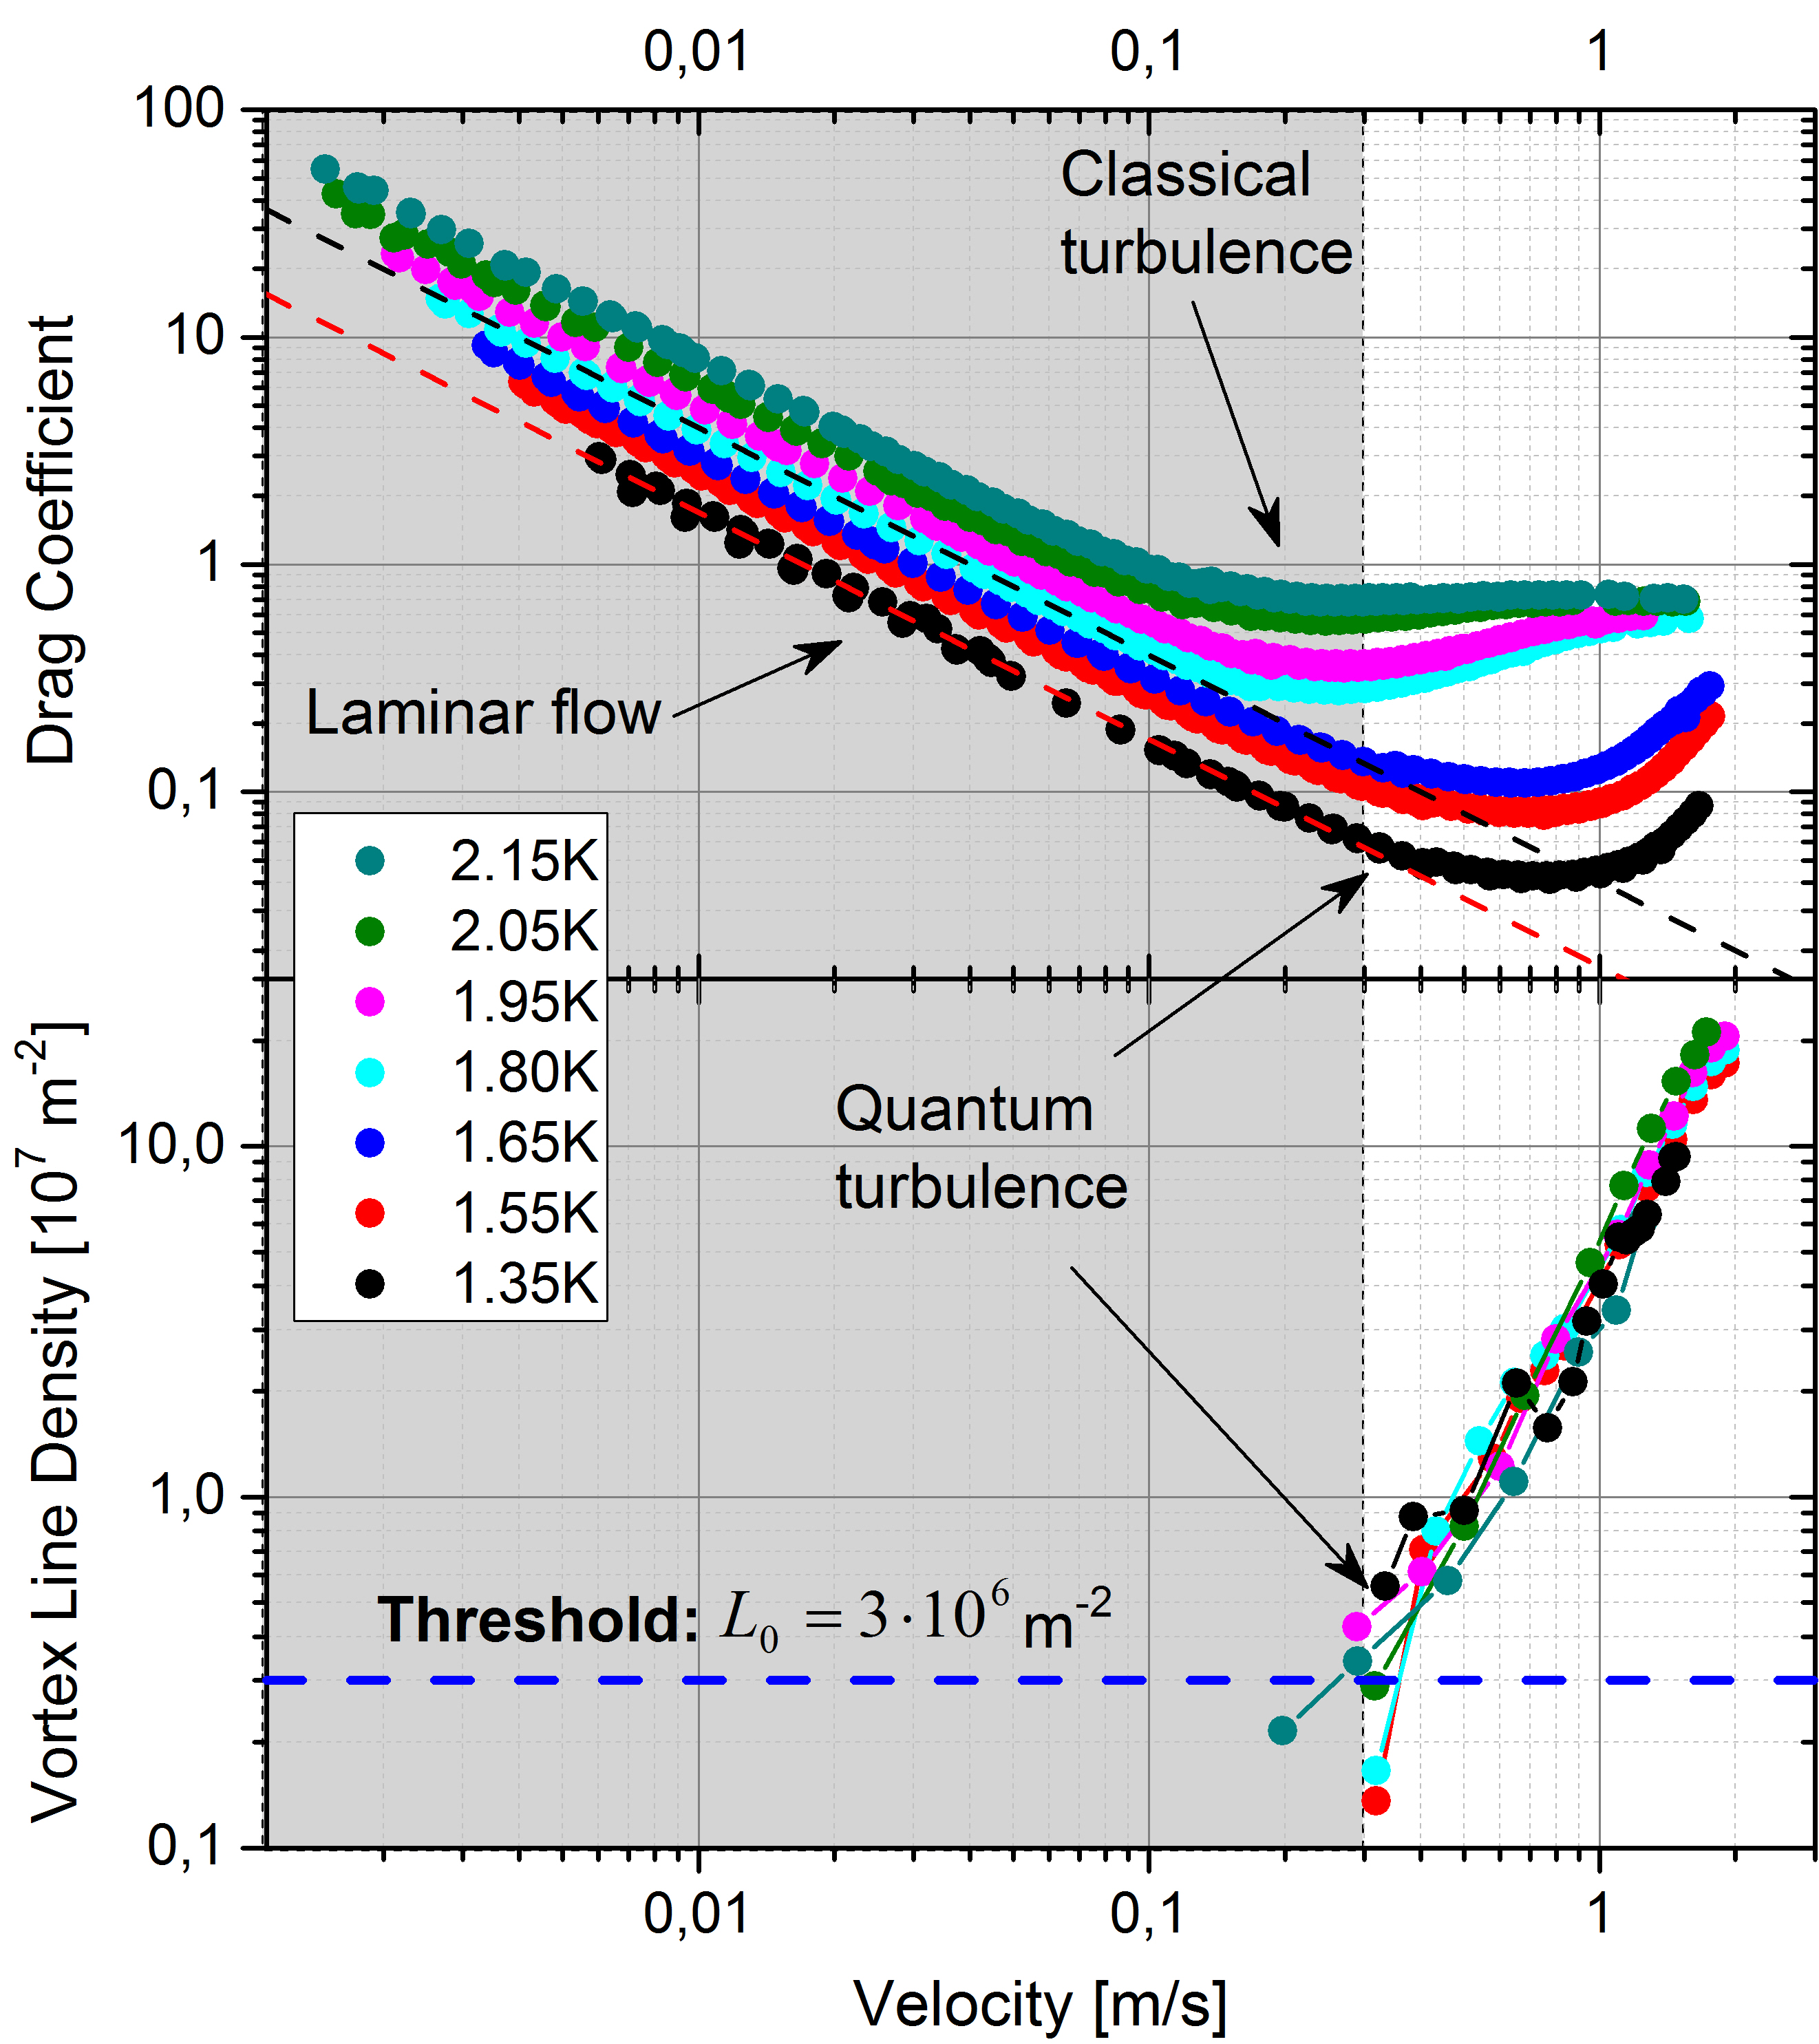
\includegraphics[width=0.8\textwidth]{graphs/Merged_C+L_fund}
	\caption{Velocity dependence of drag coefficient $ C_D $ and vortex line density $ L $ for the fundamental mode of the tuning fork. The \textit{blue, red and black dotted lines} are the threshold level and laminar drag fits for $ 1.35\unit{K} $ and $ 1.80\unit{K} $ curves, respectively. The \textit{shaded zone} marks sub-critical velocities from the point of view of detection of quantized vortices by second sound, and corresponds to the laminar drag regime for the lowest three temperatures.}
\end{figure}


In {\sffamily\textbf{Figure 3.8}} we clearly see the correlation between the production of QT (lower graph) and the onset of non-linear drag force in $ 1.35\unit{K} $, $ 1.55\unit{K} $ and $ 1.65\unit{K} $ curves. For the other curves ($ 1.80 \unit{K} $ and above), the density of normal component is much higher and consequently the critical oscillatory Reynolds number was exceeded earlier than the critical velocity $v_{\ind{c}}^{\ind f}$.

However, from {\sffamily\textbf{Figure 3.8}} we are not sure, whether QT really occurred first or CT was just too weak to be noticed by our devices. The graphs in {\sffamily\textbf{Figure 3.9}} compare the normal drag coefficient $ C_{D\ind{n}} $ and vortex line density $ L $ against $ \text{Re}_{\delta_{\ind n}} $ and better illustrate the situation. We purposely zoomed the region near transition. 


\begin{figure}[h!]
	\centering
	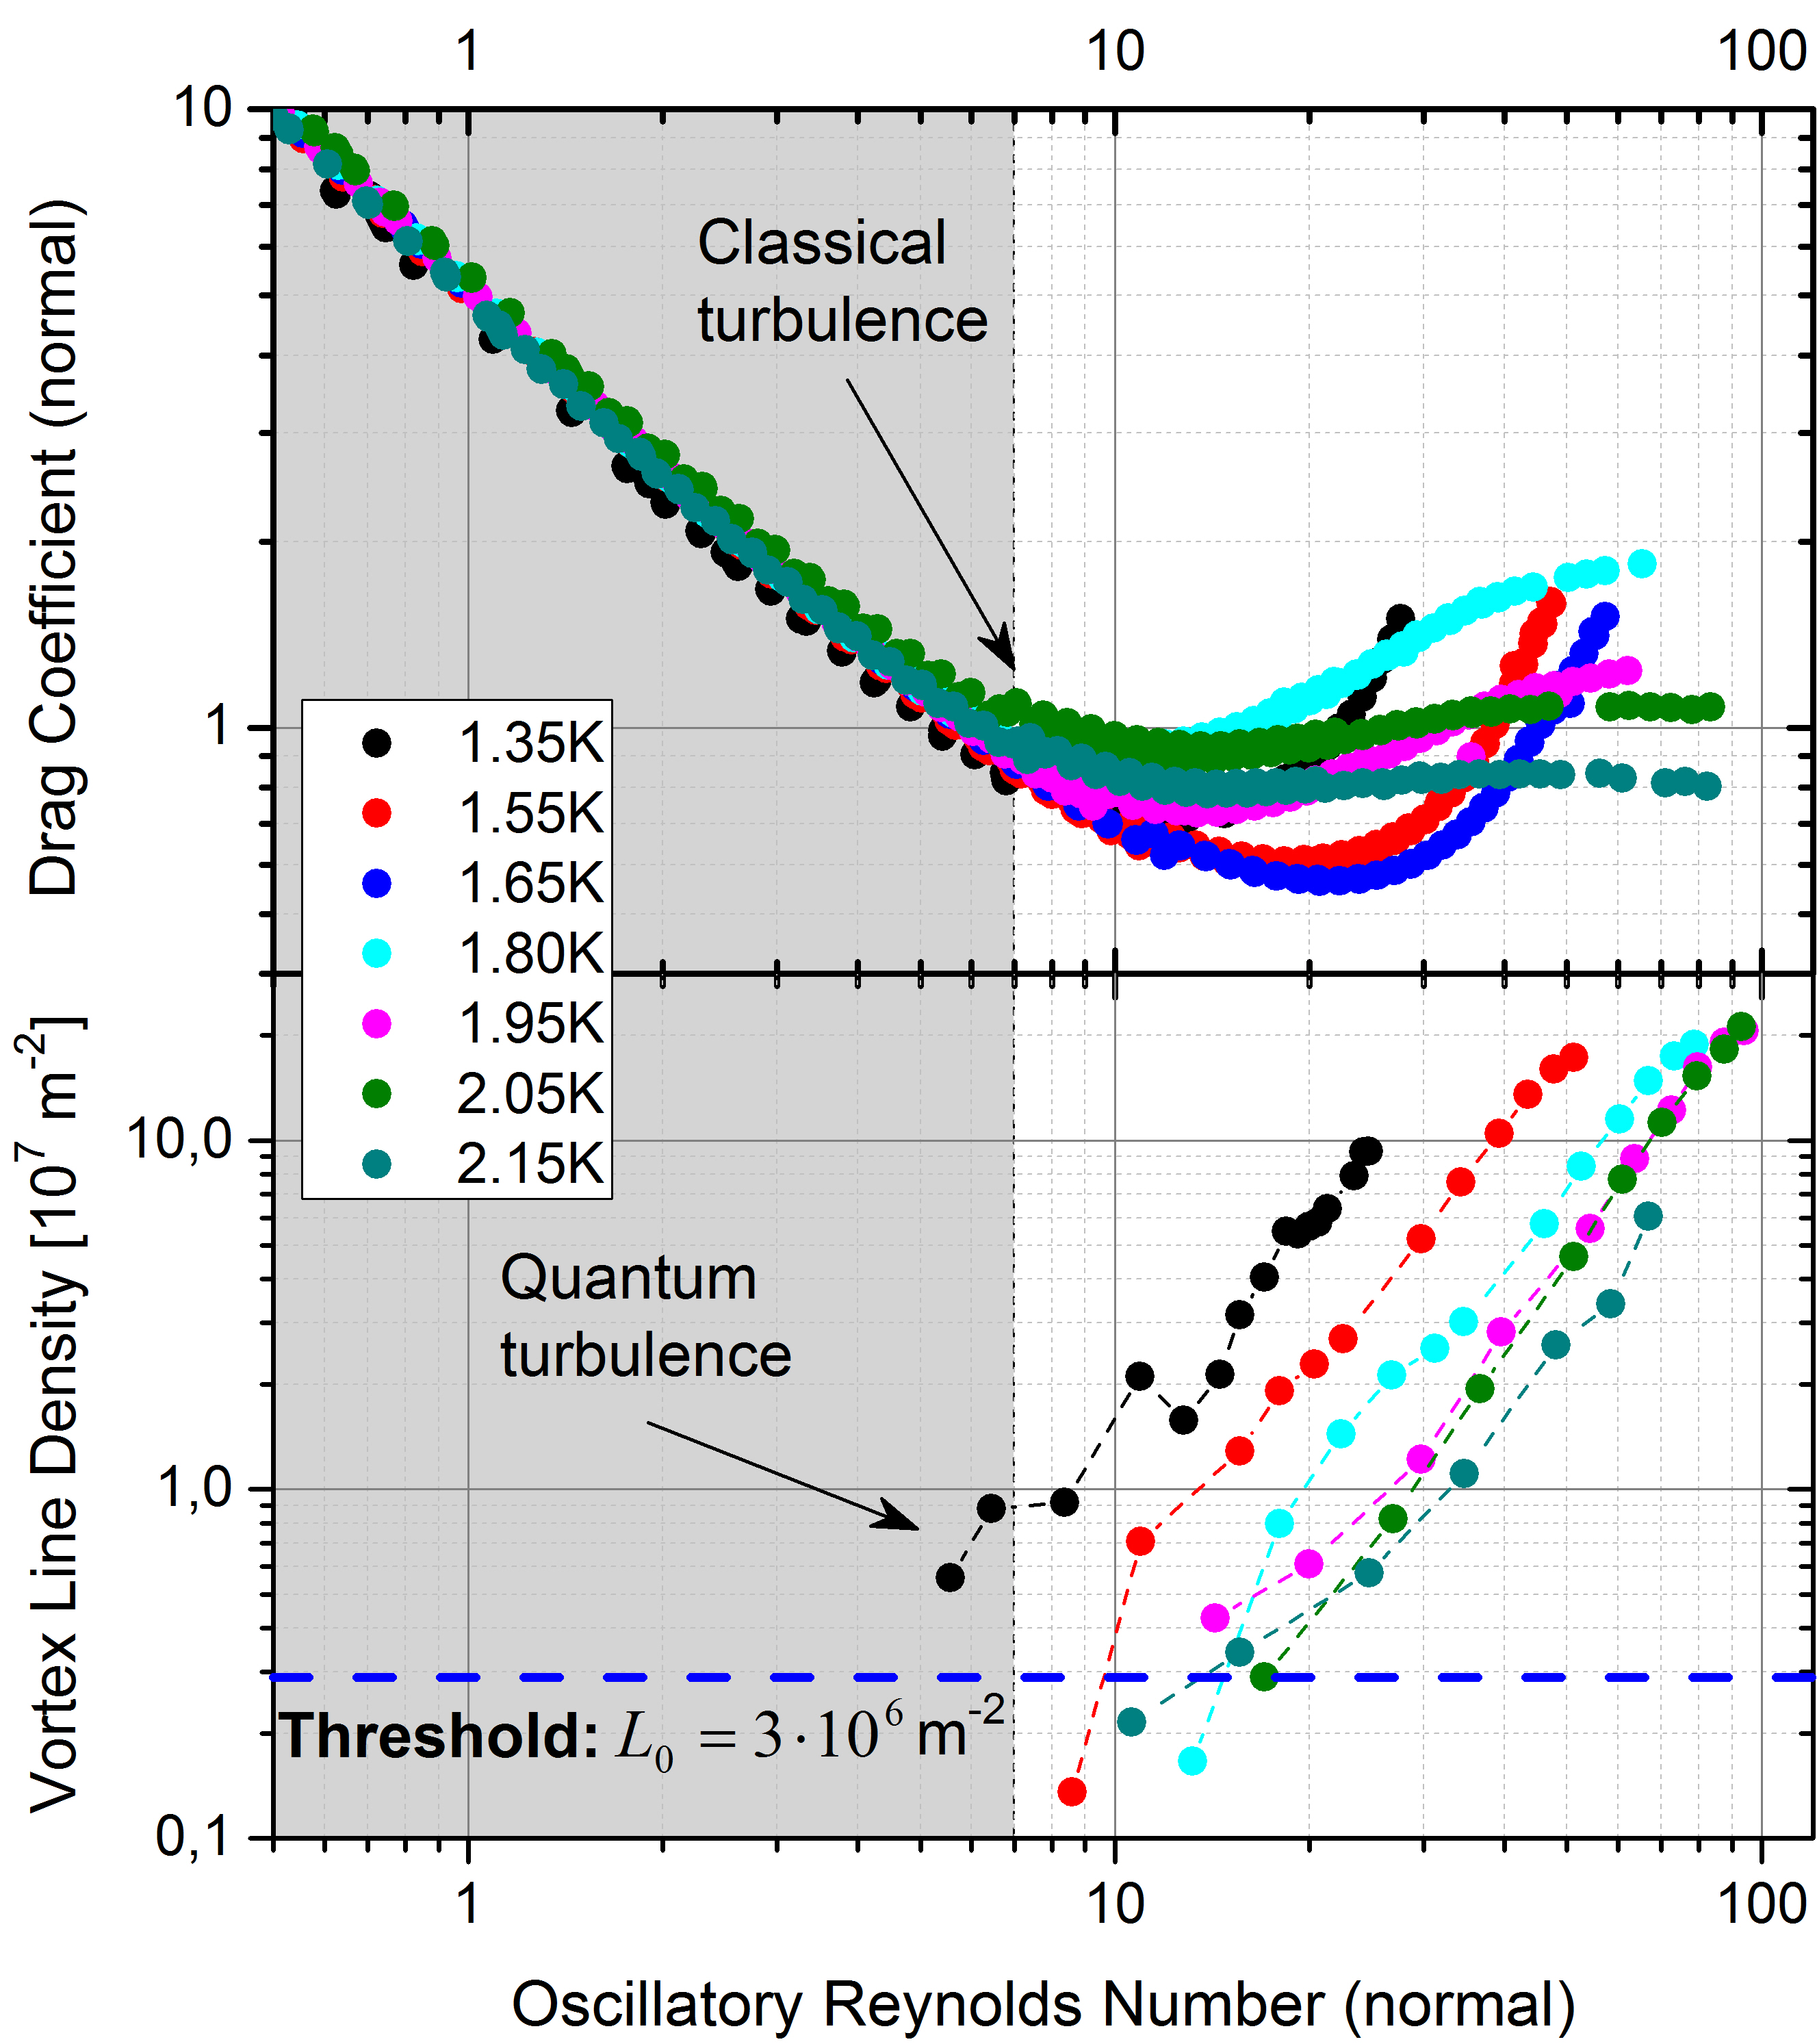
\includegraphics[width=0.8\textwidth]{graphs/Merged_C+L_Ren_fund}
	\caption{Plot of the normal fluid drag coefficient $ C_{D\ind{n}} $ and vortex line density $ L $ against the oscillatory Reynolds number $ \text{Re}_{\delta_{\ind n}} $ for the fundamental mode of tuning fork.}
\end{figure}

As shown before, classical turbulence of the normal component arises roughly when exceeding the critical $ \text{Re}_{\delta_{\ind n}c} \approx 7$. On the other hand, QT has been detected above $ v_{\ind{c}}^{\ind{f}} \approx 0.3 \unit{m/s}$, so in {\sffamily\textbf{Figure 3.9}} it is clearly shown that a considerable QT was detected as first only for temperature $ 1.35 \unit{K} $. However, following the previous set of graphs in {\sffamily\textbf{Figure 3.8}}, we came to a similar conclusion for all three of the lowest temperatures ($ 1.35 \unit{K} $, $ 1.55 \unit{K} $, $ 1.65 \unit{K} $), not just the lowest one. This could be understood in such a manner that although CT could have occurred first for $ 1.55 \unit{K} $ and $ 1.65 \unit{K} $, QT followed shortly and soon became a dominant contribution to the drag force due to the high density of the superfluid component.

\newpage


\subsection*{Overtone Mode}

Here we perform exactly the same dependencies and similar conclusions we introduced for the fundamental mode in previous {\sffamily\textbf{Section 3.3}}.

\begin{figure}[h!]
	\centering
	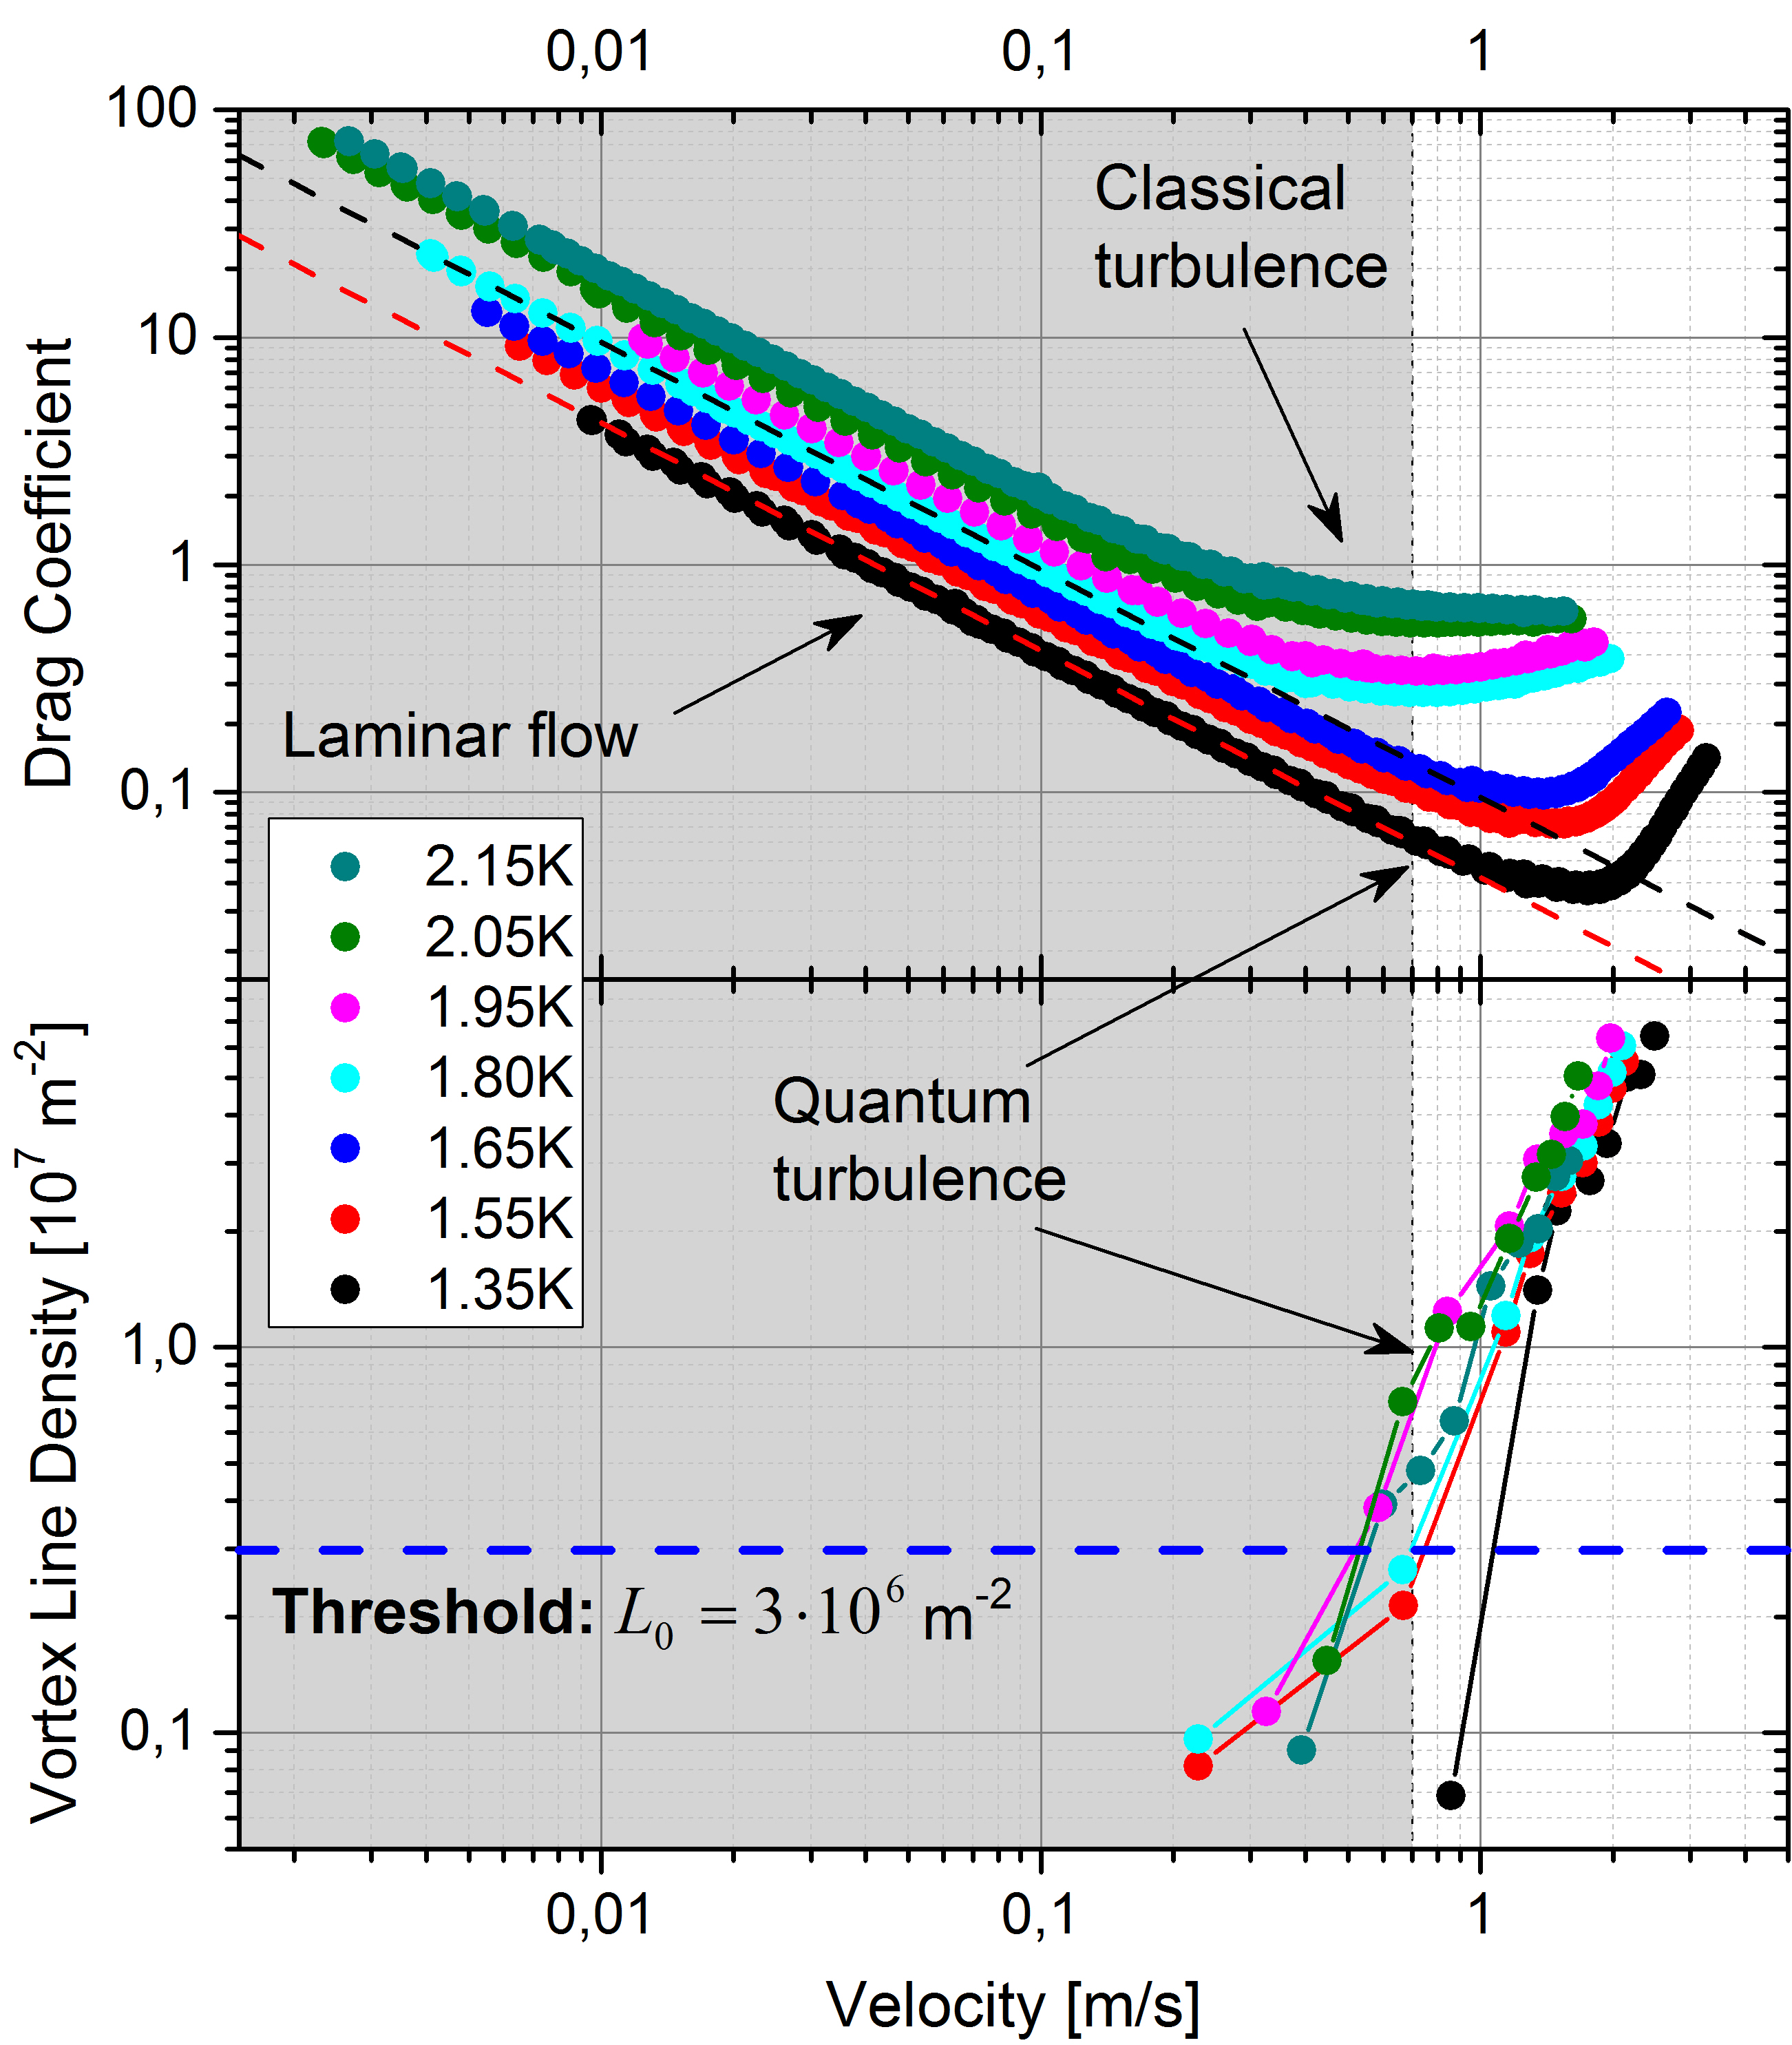
\includegraphics[width=0.8\textwidth]{graphs/Merged_C+L_over}
	\caption{Velocity dependence of drag coefficient $ C_D $ and vortex line density $ L $ for the overtone mode of the tuning fork. The \textit{blue, red and black dotted lines} are the threshold level and laminar drag fits for the $ 1.35\unit{K} $ and $ 1.80\unit{K} $ curves, respectively. The \textit{shaded zone} marks sub-critical velocities from the point of view of detection of quantized vortices by second sound, and corresponds to the laminar drag regime for the lowest three temperatures.}
\end{figure}

The situation for the overtone mode seemingly does not differ from the fundamental - the only difference is that the correlation of QT formation and onset of non-linear drag is harder to see by the naked eye.

The plots of $ C_{D\ind{n}} $ and $ L $ against $ \text{Re}_{\delta_{\ind n}} $ (shown in {\sffamily\textbf{Figure 3.11}}) will help to illustrate the order in which the turbulence transitions likely occurred.


\newpage

\begin{figure}[h!]
	\centering
	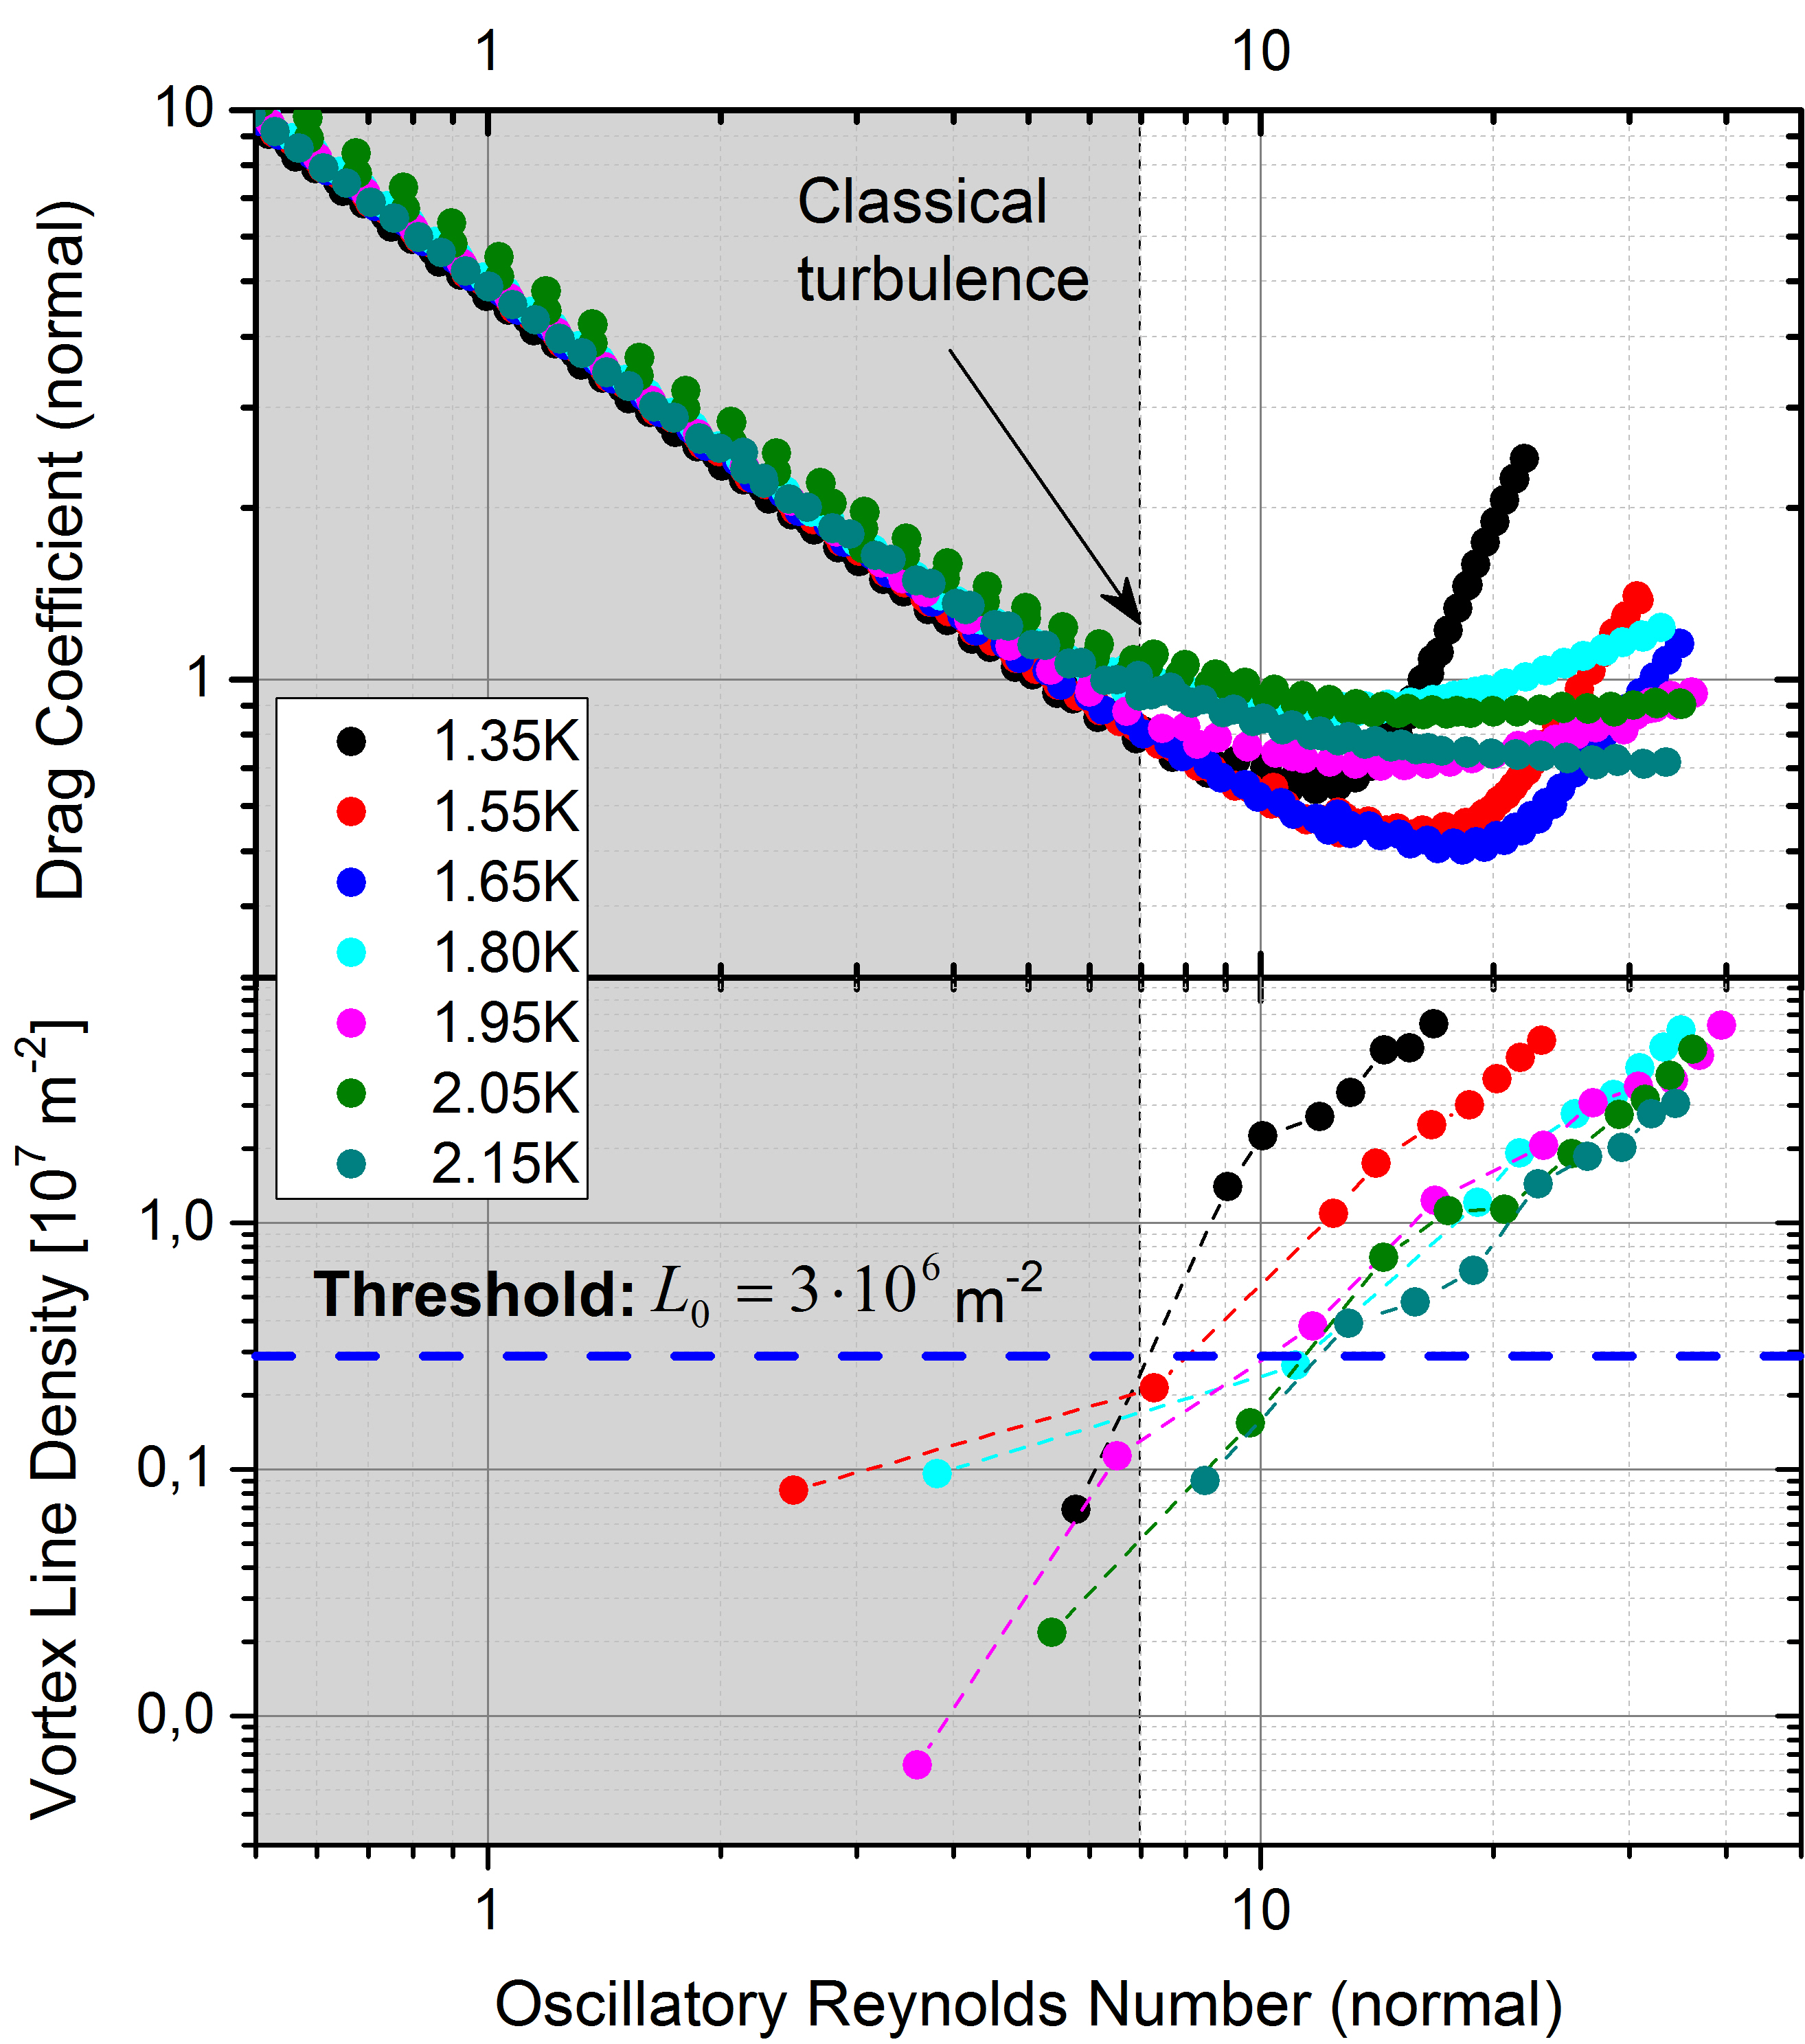
\includegraphics[width=0.8\textwidth]{graphs/Merged_C+L_Ren_over}
	\caption{Plot of the normal drag coefficient $ C_{D\ind{n}} $ and vortex line density $ L $ against the oscillatory Reynolds number $ \text{Re}_{\delta_{\ind n}} $ for the overtone mode.}
\end{figure}

In contrast with the fundamental mode, here measurable QT did not occur earlier than CT at any of the shown temperatures. Although the graph in {\sffamily\textbf{Figure 3.10}} looked like the displayed non-linearities of the lowest three temperature curves are caused due to the formation of quantized vortices, this does not necessarily have to be true. Similarly to the fundamental mode, CT may have appeared earlier, but QT dominated rapidly and hence CT could not be seen in the drag coefficients reliably.

\newpage

\section{Discussion}

In this Section we summarize all the observations and found relations between the measured drag forces and the vortex line densities detected by second sound attenuation. We also put together a \textit{flow phase diagram} for better visualisation of the whole concept. To start with, we have already found the following:

\begin{itemize}
	\item[\textbf{I.}] \textbf{Vortex line density measurement} - A significant amount of quantized vortices are produced upon exceeding the temperature-independent critical velocities $ \approx 0.3 \unit{m/s} $ and $ \approx 0.7 \unit{m/s} $ for the fundamental and overtone modes of the tuning fork, respectively. In addition, the scaling factor for critical velocity generally agrees with the prediction based on quantized vortex dynamics $ \sim \sqrt{\kappa \omega} $.
	
	\item[\textbf{II.}] \textbf{Drag force measurement} - Until a certain oscillatory Reynolds number $ \text{Re}_{\delta_{\ind n}c}=7\pm 2 $ is exceeded, the drag force is linear with velocity. For higher temperatures, where there is considerably less superfluid component, there is a clear transition to a $ C_D \approx \text{const.} $ non-linear drag, similar as in classical fluids and likely related to turbulence of the normal component. 
	
	\item[\textbf{III.}] \textbf{Correlations} - The onset of non-linearity for $ 1.35\unit{K} $, $ 1.55\unit{K} $ and $ 1.65\unit{K} $ curves is definitely caused by the production of quantized vortices, although classical turbulence of normal component appeared earlier in the most of cases, but with negligible effect on drag. In other cases ($ 1.80 \unit{K}$ and above), CT dominates as the first.
\end{itemize}


\subsection*{Flow Phase Diagram}

To have a better idea, when each of the turbulences occur, we will attempt to construct a \textit{flow phase diagram}, plotting $ \text{Re}_{\delta_{\ind n}} $ against velocity and illustrating the areas of non-linear drag forces at each temperature. For the time being, let us consider a much simplified situation where CT and QT do not affect each other, i.e., no interactions between the normal and the superfluid component. Within this first approach, QT is created only  when the critical velocity $ v_{\ind{c}}^{\ind{{f}}} = 0.3 \pm 0.1 \unit{m/s}$ (for fundamental mode) or $ v_{\ind{c}}^{\ind{{o}}} = 0.7 \pm 0.2 \unit{m/s}$ (for overtone mode) is exceeded and CT forms when exceeding the critical oscillatory Reynolds number $ \text{Re}_{\delta_{\ind n}c}=7\pm 2 $. For a more direct comparison of the two resonant modes of the tuning fork, we additionally rescale the peak velocities by the factor of $\sqrt{\kappa \omega}$, obtaining a \textit{dimensionless velocity}. Whether CT and/or QT occur or not can be then shown using rectangular \textit{turbulent zones} in a flow phase diagram combining these two quantities.

Let us recall the definition of the oscillatory Reynolds number for normal component:

\begin{equation}
	\text{Re}_{\delta_{\ind n}}(T) = \frac{\rho_{\ind n}(T)\delta_{n}(T) v}{\eta(T)}
	= \sqrt{\frac{2\kappa\eta(T)}{\rho_{\ind n}(T)}}\cdot \frac{v}{\sqrt{\kappa \omega(T)}}\,,
	\label{phase_diag}
\end{equation}
where $ \eta(T) $ and $ \rho_{\ind n}(T) $ are temperature dependent viscosity and normal fluid density (experimental values can be found in \cite{donnelly}). According to (\ref{phase_diag}), we should get in a log-log flow phase diagram a set of parallel lines for the different temperatures, intersecting the boundaries of the \textit{turbulent zones} in different order.

Needless to say, this is a gross oversimplification of the real situation, as the presence of any significant amount of quantized vortices will lead to a non-negligible mutual friction force between the two components. At the same time, pressure and velocity fluctuations in any classical turbulence of the normal component may affect the precise moment at which quantized vortices pinned to the surface of the fork start to reconnect and multiply.

\begin{figure}[h!]
	\centering
	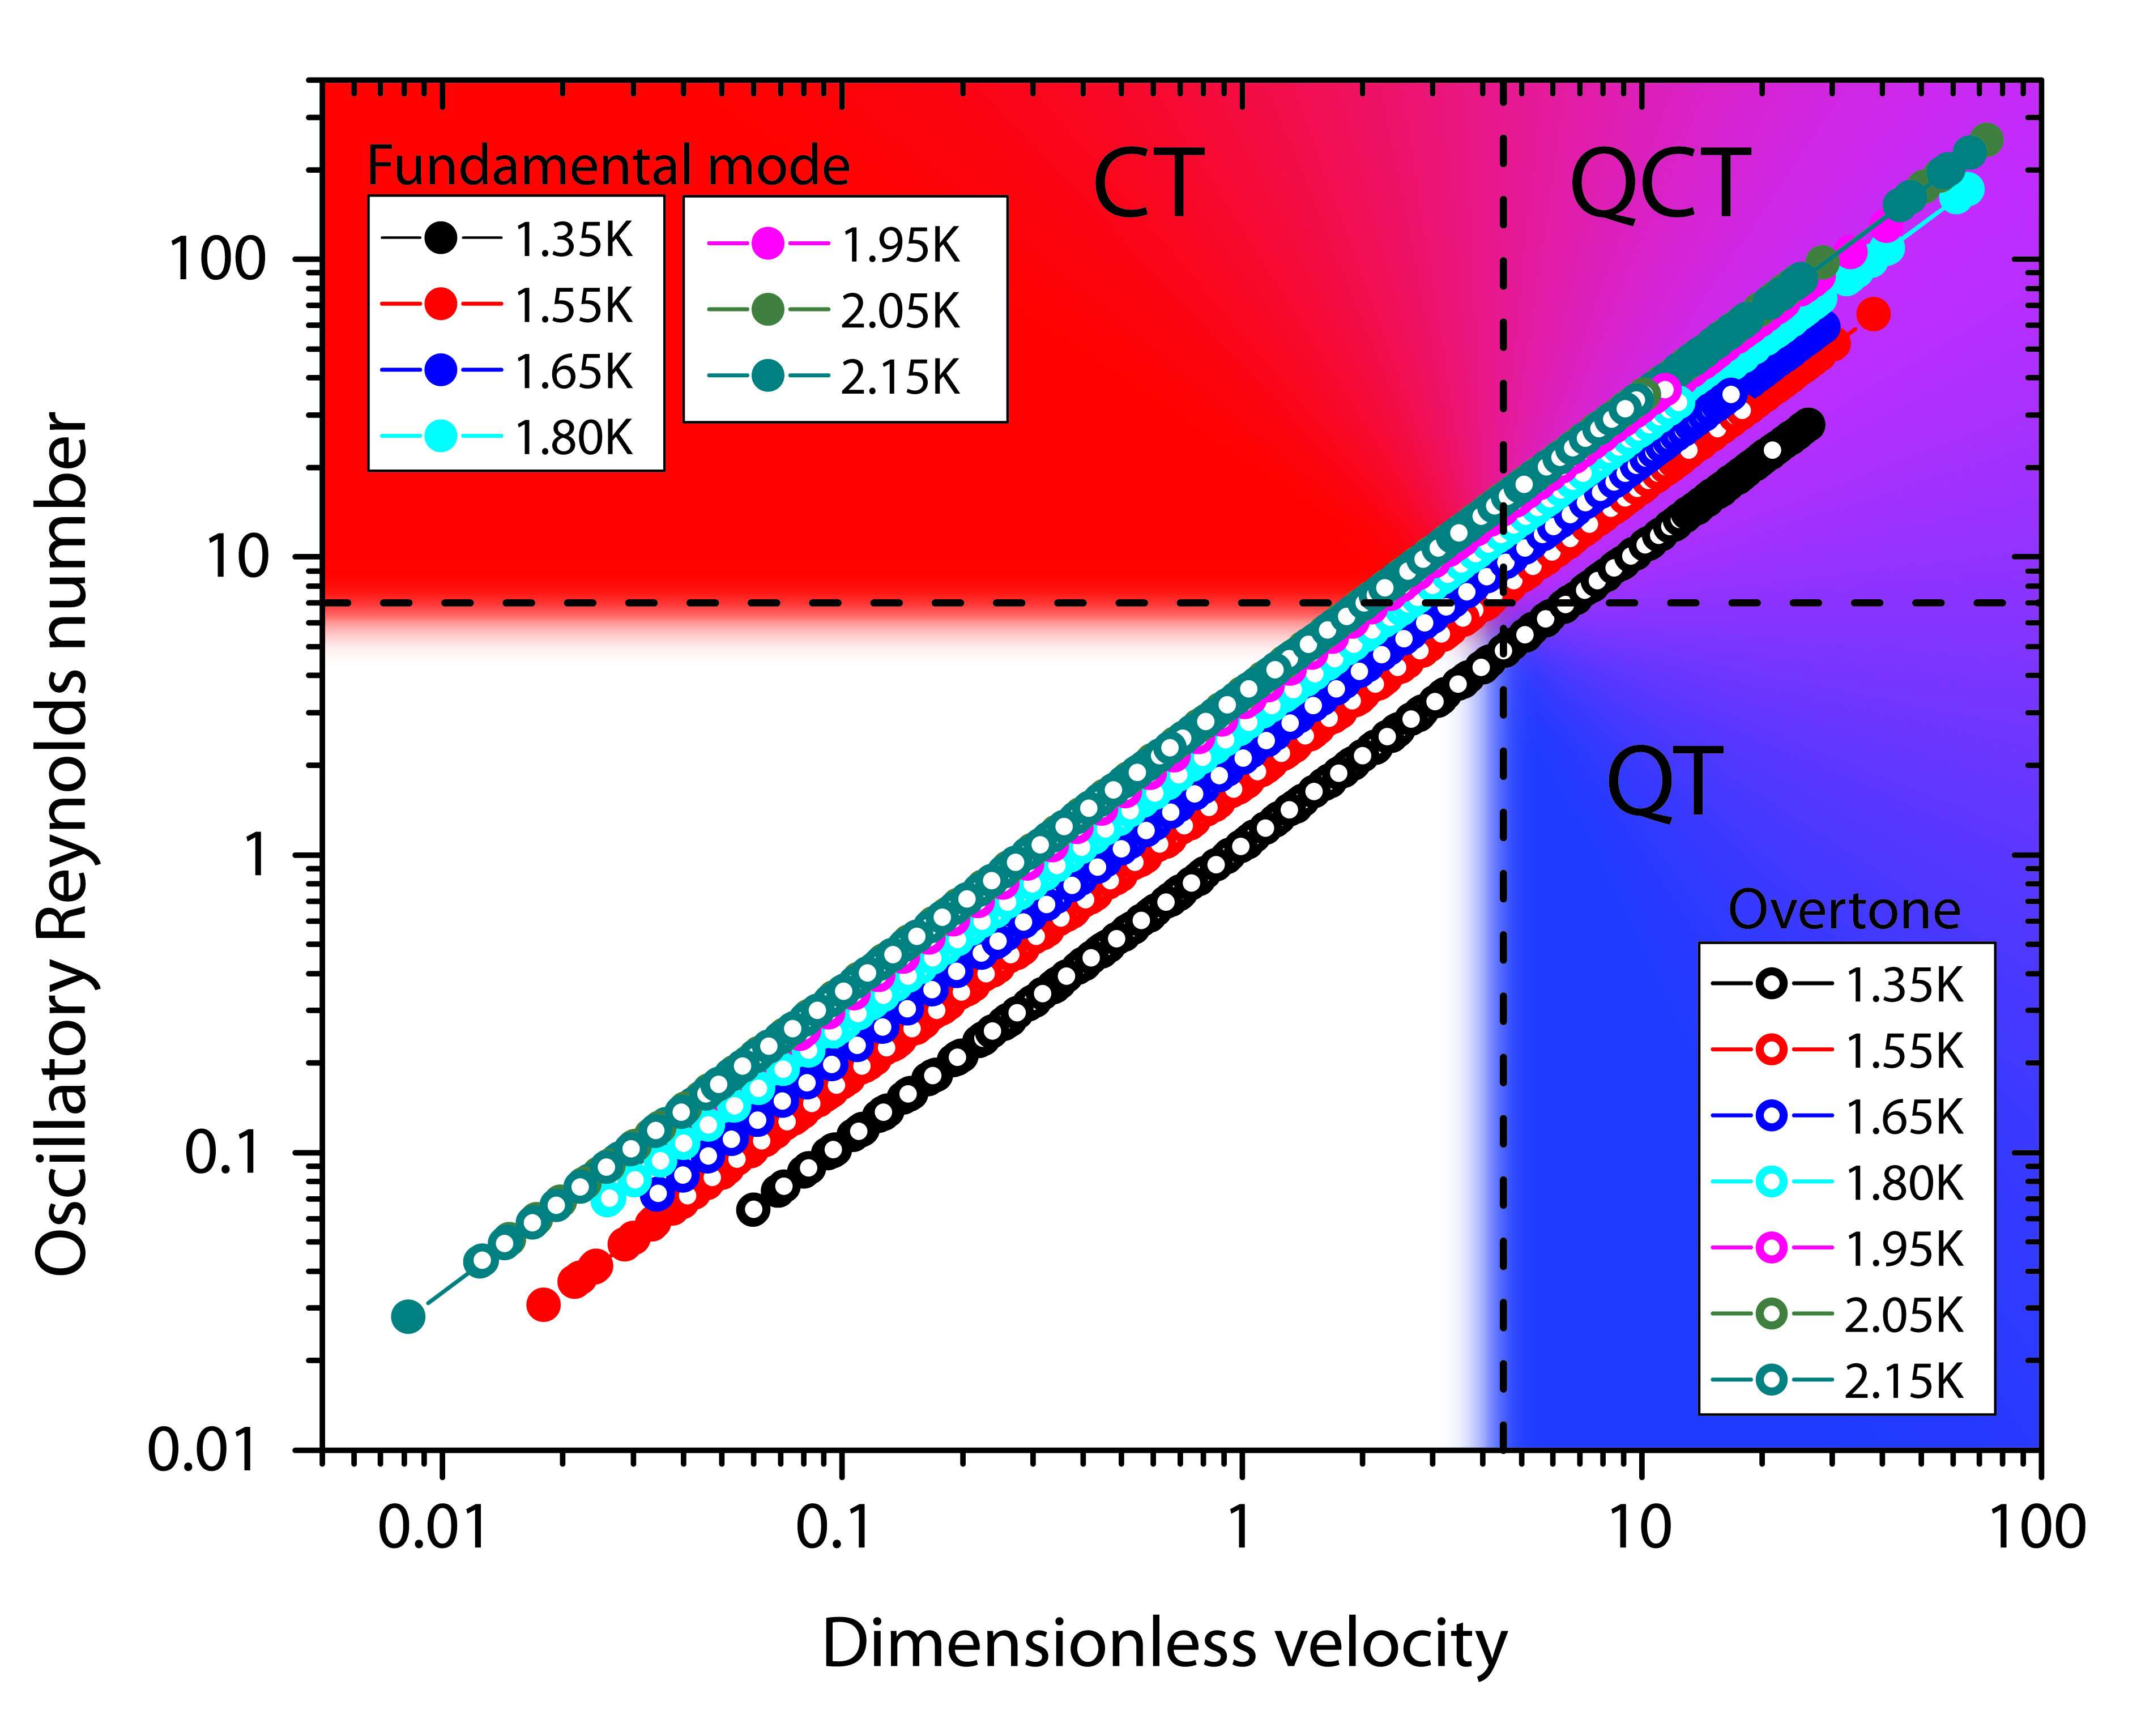
\includegraphics[width=1\textwidth]{graphs/FlowPhase_diagram}
	\caption{The simplified flow phase diagram illustrating the basic conditions for CT and QT to occur in the flow due to the investigated tuning fork. We note that only in the case of $ 1.35\unit{K} $ curve we are absolutely sure that QT was created first. The vertical and horizontal \textit{black dashed lines} marks the level of critical oscillatory Reynolds number $ \text{Re}_{\delta_{\ind n}c}\approx 7$ and dimensionless critical velocity $ v_{\ind c}^{\ind f}/\sqrt{2\pi \kappa f_0^{\ind f}} \approx v_{\ind c}^{\ind o}/\sqrt{2\pi \kappa f_0^{\ind o}} \approx 4.5$. }
\end{figure}

In reality, not only the transitions to CT and/or QT will affect (and possibly help trigger) one another, but one might also suspect that even the intensity of either type of turbulence will bear significant consequences for the other one, due to coupling of the two fluids via the mutual friction force. A more thorough analysis of these effects is clearly required and this topic will be subject of further experimental investigations in an improved realization of the experimental setup.

%\newpage

\chapter{Conclusions}

In this Thesis, we have shown data reflecting the tuning fork oscillations in superfluid $ \He $ bath (at seven different velocities - $ 1.35\unit{K} $, $ 1.55\unit{K} $, $ 1.65\unit{K} $, $ 1.80\unit{K} $, $ 1.95\unit{K} $, $ 2.05\unit{K} $, $ 2.15\unit{K} $) as well as the second sound waves propagating through the resonator. The method of second sound attenuation showed that the only relevant parameter related with production of quantized vortices is the velocity amplitude of the fork tip and the (high enough) frequency of oscillation. We estimated the critical velocities for the fundamental and overtone modes to be $ v_{\ind{c}}^{\ind f} = 0.3 \pm 0.1 \unit{m/s}$, and $ v_{\ind{c}}^{\ind o} = 0.7 \pm 0.2 \unit{m/s} $, respectively, which should scale with the frequency as $ \propto \sqrt{\kappa\omega} $. We also confirmed that this scaling is consistent with the obtained critical velocities.

Using results from drag force measurements, a transition from linear to non-linear drag was clearly observed at different velocities for given temperatures. Scaling the force to drag coefficient and the velocity to oscillatory Reynolds number, both with respect to the normal component of $ \He $, revealed many hydrodynamic properties of the system. Starting with the fact that only the normal component contributes to the drag force in laminar flow, continuing with dynamical similarity of both fork modes and ending with critical $\text{Re}_{\delta_{\ind n}c}=7\pm 2 $, above which the non-linear drag was apparent.

We divided the temperature curves in two categories - those for which the non-linearity seemingly appeared at one certain velocity (strongly correlated with the production of quantized vortices), and those for which the onset arises when exceeding the critical $\text{Re}_{\delta_{\ind n}c}$. More detailed analysis showed that in the case of fundamental mode, we can safely claim that QT occurred first only for $ T = 1.35\unit{K} $. For the overtone mode, this scenario actually could not be confirmed for any temperature at all. But we have to still keep in mind that due to a relatively high sensitivity threshold and less-than-optimal quality of the second sound signal, it is, at this point, difficult to arrive at more convincing conclusions. 

Finally, we introduced the \textit{flow phase diagram} as a good illustrative tool showing each type of turbulence in particular \textit{zones} and each of the temperature curves as a set of parallel lines, intersecting the boundaries of \textit{zones} in different order.

\subsection*{Summary}

We summarize all the achieved results and conclusions (denoting "$ \checkmark $" as a positive contribution, "\textbf{?}" as an unresolved question and "$ \times $" as an aspect that should be improved in future) as follows:


\begin{itemize}

	
	\item[\checkmark] Fundamental and overtone resonance mode of submerged tuning fork in superfluid $ \He $ have been found ($ f_0^{\text{f}} = 6.38\unit{kHz} $, $ f_0^{\text{o}} = 40.00\unit{kHz} $).
	
	\item[\checkmark] Second sound has been generated and a wide frequency sweep measured. The $ 1^{\ind{st}} $ mode appeared to be the clearest and was used in further measurements.
	
	\item[\checkmark] Reliable formation of quantum turbulence above $ v_{\ind{c}}^{\ind{{f}}} = 0.3 \pm 0.1 \unit{m/s}$ (fundamental) and $ v_{\ind{c}}^{\ind{{o}}} = 0.7 \pm 0.2 \unit{m/s}$ (overtone) was found to be temperature independent.
	
	\item[\checkmark] The theory of critical velocity scaling $ v_{\ind{c}} \propto \sqrt{\kappa\omega}$ has been found in agreement with the experimental results.
	
	\item[\checkmark] We obtained data across 4 orders of magnitude in the dimensionless velocity (from $ 10^{-2} $ to 100), which is a remarkably wide range.
	
	\item[\checkmark] The oscillatory Reynolds number defined for normal component of superfluid $ \He $ as $\text{Re}_{\delta_{\ind n}} = \rho_{\ind n}\delta_{n} v/\eta$ proved to lead to the correct scaling of the drag forces and turned out to be a useful quantity in our analysis.
	
	\item[\checkmark] Onset of non-linear drag has been observed above $ \text{Re}_{\delta_{\ind n}c}=7\pm 2 $ for both fork modes.
	
	\item[\checkmark] QT definitely occurs before CT at $ 1.35\unit{K} $, while CT occurs first at $ 2.15\unit{K} $ and $ 2.05\unit{K} $. This means that a temperature must exist between these two values, where both types of turbulence are likely to be created at the same time. With the data available, we can estimate this temperature to be close to $ 1.52\unit{K} $ for the tuning fork used in this study.
	
	\item[\textbf{?}] Except for the outermost temperatures, we cannot say with certainty which type of turbulence appears first.

	\item[\textbf{?}] The true shape of the \textit{turbulence zones} is still not clear. Without better-resolved measurements, we have only a rough estimate based on the critical velocities and the oscillatory Reynolds number (which may themselves be affected by the sensitivity of the second sound resonator and the unsystematic behaviour of the tuning forks).
	
	\item[$\times$] The sensitivity and quality of second sound sensors should be improved to provide less deviation of critical velocities. This may be achieved, e.g., by using a shorter resonator without a strong connection to the helium bath as the current one had (a 1~mm diameter hole).
	
	\item[$ \times $] The unsystematic behaviour of the tuning fork ought to be eliminated. We believe that this is indeed possible, as other experiments with the same tuning fork (even measurements on the dilution fridge in the Prague Laboratory of Superfludity) have shown no signs of such behaviour. The first steps to be taken is a better isolation of the tuning forks and the entire second sound resonator from the helium bath, such as in a pressure cell or inside an enclosure filled by helium only through superleaks.
\end{itemize}

This topic (identification of the onset of the different types of turbulence) will definitely need much more experimental (and theoretical) work to clarify what are the conditions to make QT or CT and how these effects can interact.
%% Norma citácii: ISO 690

\def\bibname{Bibliography}
\begin{thebibliography}{99}
	\addcontentsline{toc}{chapter}{\bibname}
	
\bibitem{kapitsa}
{\sc Kapitsa, P.}
\emph{The Super-Fluidity of Liquid Helium II}.
Nature \textbf{141}, 74 (1938)

\bibitem{tong}
{\sc Tong, D.}
\emph{Statistical physics}.
University of Cambridge Part II

\bibitem{tisza}
{\sc Tisza, L.}
\emph{The viscosity of liquid helium and the Bose-Einstein statistics.}\\
Comptes Rendus Acad. Sciences, \textbf{207}:1186-1189 (1952)

\bibitem{landau}
{\sc Landau, L.D.} \text{and} {\sc Lifshitz, E.M.}
\emph{Fluid Mechanics}, Second English Edition.\\
Pergamon Books Ltd., (1987). \mbox{ISBN~0-08-033933-6}

\bibitem{landau_superfluid}
{\sc Landau, L.D.}
\emph{The theory of superfluidity of helium II}.\\
J. Phys. USSR, Vol. \textbf{11}, 91 (1947)

\bibitem{andro}
{\sc Andronikashvili, E.L.}
J. Phys. USSR, \textbf{10}, 201 (1946)


\bibitem{skrbek}
{\sc Skrbek, L.} et al.
\emph{Fyzika nízkých teplot}, 1. vydání.\\
Praha: {\sl MatfyzPress}, (2011). \mbox{ISBN~978-80-7378-168-2}.

\bibitem{varga}
{\sc Varga, E.}
\emph{Second sound as a tool to study He-II flow}.
Bachelor thesis (2012).	

\bibitem{osborne}
{\sc Osborne, D.V.}
\emph{The Rotation of Liquid Helium-II}.

Proc. Royal Soc. London , \textbf{63}: 909-912 (1950)

\bibitem{feynman}
{\sc Feynman, R.}.
\emph{Application of quantum mechanics to liquid helium}.\\
Progress in Low Temperature Physics, \textbf{1}, 17-53 (1957)

\bibitem{tony}
{\sc Guénault, T.}
\emph{Basic Superfluids}.\\
Taylor $\&$ Francis e-Library (2003). ISBN~0-203-26973-X.

\bibitem{vinen1}
{\sc Vinen, W.F.} and {\sc Hall, H.E.}
\emph{The rotation of liquid helium II}

I.\hspace{2mm}\emph{Experiments on the propagation of second sound in uniformly rotating helium II}.

Proc. Royal Soc. London \textbf{238}:204-214 (1957) 

\bibitem{vinen2}
{\sc Vinen, W.F.} and {\sc Hall, H.E.}
\emph{The rotation of liquid helium II}

II.\hspace{2mm}\emph{The theory of mutual friction in uniformly rotating helium II}.

Proc. Royal Soc. London \textbf{238}:215-234 (1957)

\bibitem{physrevB}
{\sc S. Babuin , M. Stammeier, E. Varga, M. Rotter, L. Skrbek  }
\emph{Quantum turbulence of bellows-driven $\He$ superflow: Steady state} Phys. Rev. B, \textbf{86} (2012)

\bibitem{turbulence}
{\sc Van Dyke, M.}
\emph{An Album of Fluid Motion}.\\
The Parabolic Press, Stanford, California (1982). ISBN 0-915760-02-9

\bibitem{schoepe}
{\sc R. Hänninen, W. Schoepe}
\emph{Dynamical Scaling of the Critical Velocity for the Onset of Turbulence in Oscillatory Superflows}.
J. Low Temp. Phys. \textbf{164}: 1-4 (2011)

\bibitem{forks}
{\sc R. Blaauwgeers} \text{and col.}
\emph{Quartz tuning fork: Thermometer, Pressure- and Viscometer for Helium Liquids} Journal of low. temp. phys., Vol. \textbf{146}, (2007)

\bibitem{acoustic}
{\sc R.I. Bradleys, D. Schmoranzer} \text{and col.}
\emph{Crossover from hydrodynamic to acoustic drag on quartz tuning forks in normal and superfluid $ \He $}. Phys. Rev. B, \textbf{85} (2012)

\bibitem{donnelly} 
{\sc Donnelly, R.J., Barenghi, C.F}
\emph{The Observed Properties of Liquid Helium at the Saturated Vapor Pressure}. American Ins. of Phys. and Chem. Soc. (1998)

\bibitem{lancaster}
{\sc Ahlstorm, S.L., Brandley, D.I.} \text{and col.}.
\emph{Frequency-dependent drag from quantum turbulence produced by quartz tuning forks in superfluid $ \He $}.
Phys. Rev. B, \textbf{89} (2014)

\bibitem{history}
{\sc Brandley, D.I., Guénault, A.M.} \text{and col.}
\emph{History Dependence of Turbulence Generated by a Vibrating Wire in Superfluid $ \He $ at $ 1.5\unit{K} $}.\\
J. Low Temp. Phys. \textbf{162}:375-382 (2011)

\bibitem{Emilfluids}
{\sc Varga, E., Babuin, S., Skrbek, L.}
\emph{Second-sound studies of coflow and counterflow of superfluid $ \He $ in channels}.
Physics of fluids \textbf{27} (2015)

\bibitem{opticalfork}
{\sc Bradley, D.I., Crookston, P.} \text{and col.}
\emph{Measuring the Prong Velocity of Quartz Tuning Forks Used to Probe Quantum Fluids}.
J. Low Temp. Phys. \textbf{161}:536-547 (2010)

\bibitem{PraguePRB}
{\sc Blažková, M., Schmoranzer, D.} \text{and col.}
\emph{Generation of turbulence by vibrating forks and other structures in superfluid $ \He $}.
Phys. Rev. B, \textbf{79} (2009)

\bibitem{jackson} 
{\sc Jackson, M.J.} \text{and col.}
\emph{Measurement of Vortex Line Density Generated by a Quartz Tuning Fork in Superfluid $ \He $}
J. Low Temp. Phys. \textbf{183}:208-214 (2016)

\bibitem{bahyl}
{\sc Bahyl, J.}
\emph{Measurement of quantum turbulence in superfluid $ \He $}.
FMFI ŠVK (2016)
	
	
	
\end{thebibliography}

\chapter*{Introduction / Motivation (3 pgs)}
\addcontentsline{toc}{chapter}{Introduction}

\begin{itemize}
	\item helium backround, phase diagram, superfluid transition, interesting properties
	\item quantum turbulence, comparison with classical turbulence
	\item overview on experiments with QT
	\item overview on numerical simulations of QT
	\item motivations, goals of this work
\end{itemize}

\newpage
\chapter{Theoretical Background (15 pgs)}

The theoretical part of this Thesis is composed of three chapters:

\begin{itemize}
	\item[1.] Microscopic view - wave function, collapse, quantum vortices

	\item[2.] Mesoscopic view - filaments, drag and magnus force, dynamics of vortex, Schwarz equation, Kelvin waves (?)

	\item[3.] Macroscopic view - hydrodynamics, two-fluid model, 

\end{itemize}
\vspace{1cm}

\newpage

{\Huge \bfseries Microscopic model}
\addcontentsline{toc}{chapter}{Microscopic model}
\vspace{0.3cm}

\section{Bose-Einstein condensate}

\section{Quantum vortex properties}

{\Huge \bfseries Mesoscopic model}
\addcontentsline{toc}{chapter}{Mesoscopic model}
\vspace{0.3cm}

\section{Filaments theory}

\section{Filaments dynamics}

{\Huge \bfseries Macroscopic model}
\addcontentsline{toc}{chapter}{Macroscopic model}
\vspace{0.3cm}

\section{Two-fluid model}

\section{Oscillatory motion}

\section{Quantum turbulence}

\section{Quantum rings}

\newpage

\chapter{Experimental Setup (20 pgs)}

\section{Apparatus}

\section{QT Generators}

\subsection*{Quartz Tuning Fork}

\section{Measurements and Processing}

\section{Scaling, Second Sound}

\newpage

\chapter{Simulations (15 pgs)}

\section{Codebase}

\section{Finite differences}

\section{Stepping}

\section{Resegmentation}

\section{Vortex ring}

\newpage

\chapter{Results (10 pgs)}

\section{Experiments}

\section{Simulations}

\newpage

% Norma citácii: ISO 690

\def\bibname{Bibliography}
\begin{thebibliography}{99}
	\addcontentsline{toc}{chapter}{\bibname}
	
\bibitem{kapitsa}
{\sc Kapitsa, P.}
\emph{The Super-Fluidity of Liquid Helium II}.
Nature \textbf{141}, 74 (1938)

\bibitem{tong}
{\sc Tong, D.}
\emph{Statistical physics}.
University of Cambridge Part II

\bibitem{tisza}
{\sc Tisza, L.}
\emph{The viscosity of liquid helium and the Bose-Einstein statistics.}\\
Comptes Rendus Acad. Sciences, \textbf{207}:1186-1189 (1952)

\bibitem{landau}
{\sc Landau, L.D.} \text{and} {\sc Lifshitz, E.M.}
\emph{Fluid Mechanics}, Second English Edition.\\
Pergamon Books Ltd., (1987). \mbox{ISBN~0-08-033933-6}

\bibitem{landau_superfluid}
{\sc Landau, L.D.}
\emph{The theory of superfluidity of helium II}.\\
J. Phys. USSR, Vol. \textbf{11}, 91 (1947)

\bibitem{andro}
{\sc Andronikashvili, E.L.}
J. Phys. USSR, \textbf{10}, 201 (1946)


\bibitem{skrbek}
{\sc Skrbek, L.} et al.
\emph{Fyzika nízkých teplot}, 1. vydání.\\
Praha: {\sl MatfyzPress}, (2011). \mbox{ISBN~978-80-7378-168-2}.

\bibitem{varga}
{\sc Varga, E.}
\emph{Second sound as a tool to study He-II flow}.
Bachelor thesis (2012).	

\bibitem{osborne}
{\sc Osborne, D.V.}
\emph{The Rotation of Liquid Helium-II}.

Proc. Royal Soc. London , \textbf{63}: 909-912 (1950)

\bibitem{feynman}
{\sc Feynman, R.}.
\emph{Application of quantum mechanics to liquid helium}.\\
Progress in Low Temperature Physics, \textbf{1}, 17-53 (1957)

\bibitem{tony}
{\sc Guénault, T.}
\emph{Basic Superfluids}.\\
Taylor $\&$ Francis e-Library (2003). ISBN~0-203-26973-X.

\bibitem{vinen1}
{\sc Vinen, W.F.} and {\sc Hall, H.E.}
\emph{The rotation of liquid helium II}

I.\hspace{2mm}\emph{Experiments on the propagation of second sound in uniformly rotating helium II}.

Proc. Royal Soc. London \textbf{238}:204-214 (1957) 

\bibitem{vinen2}
{\sc Vinen, W.F.} and {\sc Hall, H.E.}
\emph{The rotation of liquid helium II}

II.\hspace{2mm}\emph{The theory of mutual friction in uniformly rotating helium II}.

Proc. Royal Soc. London \textbf{238}:215-234 (1957)

\bibitem{physrevB}
{\sc S. Babuin , M. Stammeier, E. Varga, M. Rotter, L. Skrbek  }
\emph{Quantum turbulence of bellows-driven $\He$ superflow: Steady state} Phys. Rev. B, \textbf{86} (2012)

\bibitem{turbulence}
{\sc Van Dyke, M.}
\emph{An Album of Fluid Motion}.\\
The Parabolic Press, Stanford, California (1982). ISBN 0-915760-02-9

\bibitem{schoepe}
{\sc R. Hänninen, W. Schoepe}
\emph{Dynamical Scaling of the Critical Velocity for the Onset of Turbulence in Oscillatory Superflows}.
J. Low Temp. Phys. \textbf{164}: 1-4 (2011)

\bibitem{forks}
{\sc R. Blaauwgeers} \text{and col.}
\emph{Quartz tuning fork: Thermometer, Pressure- and Viscometer for Helium Liquids} Journal of low. temp. phys., Vol. \textbf{146}, (2007)

\bibitem{acoustic}
{\sc R.I. Bradleys, D. Schmoranzer} \text{and col.}
\emph{Crossover from hydrodynamic to acoustic drag on quartz tuning forks in normal and superfluid $ \He $}. Phys. Rev. B, \textbf{85} (2012)

\bibitem{donnelly} 
{\sc Donnelly, R.J., Barenghi, C.F}
\emph{The Observed Properties of Liquid Helium at the Saturated Vapor Pressure}. American Ins. of Phys. and Chem. Soc. (1998)

\bibitem{lancaster}
{\sc Ahlstorm, S.L., Brandley, D.I.} \text{and col.}.
\emph{Frequency-dependent drag from quantum turbulence produced by quartz tuning forks in superfluid $ \He $}.
Phys. Rev. B, \textbf{89} (2014)

\bibitem{history}
{\sc Brandley, D.I., Guénault, A.M.} \text{and col.}
\emph{History Dependence of Turbulence Generated by a Vibrating Wire in Superfluid $ \He $ at $ 1.5\unit{K} $}.\\
J. Low Temp. Phys. \textbf{162}:375-382 (2011)

\bibitem{Emilfluids}
{\sc Varga, E., Babuin, S., Skrbek, L.}
\emph{Second-sound studies of coflow and counterflow of superfluid $ \He $ in channels}.
Physics of fluids \textbf{27} (2015)

\bibitem{opticalfork}
{\sc Bradley, D.I., Crookston, P.} \text{and col.}
\emph{Measuring the Prong Velocity of Quartz Tuning Forks Used to Probe Quantum Fluids}.
J. Low Temp. Phys. \textbf{161}:536-547 (2010)

\bibitem{PraguePRB}
{\sc Blažková, M., Schmoranzer, D.} \text{and col.}
\emph{Generation of turbulence by vibrating forks and other structures in superfluid $ \He $}.
Phys. Rev. B, \textbf{79} (2009)

\bibitem{jackson} 
{\sc Jackson, M.J.} \text{and col.}
\emph{Measurement of Vortex Line Density Generated by a Quartz Tuning Fork in Superfluid $ \He $}
J. Low Temp. Phys. \textbf{183}:208-214 (2016)

\bibitem{bahyl}
{\sc Bahyl, J.}
\emph{Measurement of quantum turbulence in superfluid $ \He $}.
FMFI ŠVK (2016)
	
	
	
\end{thebibliography}


\end{document}
